%definira klasu dokumenta 
\documentclass[12pt]{report} 

%prostor izmedu naredbi \documentclass i \begin{document} se zove uvod. U njemu se nalaze naredbe koje se odnose na cijeli dokument

%osnovni LaTex ne može riješiti sve probleme, pa se koriste različiti paketi koji olakšavaju izradu željenog dokumenta
\usepackage[croatian]{babel} 
\usepackage{amssymb}
\usepackage{amsmath}
\usepackage{txfonts}
\usepackage{mathdots}
\usepackage{titlesec}
\usepackage{array}
\usepackage{lastpage}
\usepackage{etoolbox}
\usepackage{tabularray}
\usepackage{color, colortbl}
\usepackage{adjustbox}
\usepackage{geometry}
\usepackage[classicReIm]{kpfonts}
\usepackage{hyperref}
\usepackage{fancyhdr}

\usepackage{float}
\usepackage{setspace}
\restylefloat{table}


\patchcmd{\chapter}{\thispagestyle{plain}}{\thispagestyle{fancy}}{}{} %redefiniranje stila stranice u paketu fancyhdr

%oblik naslova poglavlja
\titleformat{\chapter}{\normalfont\huge\bfseries}{\thechapter.}{20pt}{\Huge}
\titlespacing{\chapter}{0pt}{0pt}{40pt}


\linespread{1.3} %razmak između redaka

\geometry{a4paper, left=1in, top=1in,}  %oblik stranice

\hypersetup{ colorlinks, citecolor=black, filecolor=black, linkcolor=black,	urlcolor=black }   %izgled poveznice


%prored smanjen između redaka u nabrajanjima i popisima
\newenvironment{packed_enum}{
	\begin{enumerate}
		\setlength{\itemsep}{0pt}
		\setlength{\parskip}{0pt}
		\setlength{\parsep}{0pt}
	}{\end{enumerate}}

\newenvironment{packed_item}{
	\begin{itemize}
		\setlength{\itemsep}{0pt}
		\setlength{\parskip}{0pt}
		\setlength{\parsep}{0pt}
	}{\end{itemize}}




%boja za privatni i udaljeni kljuc u tablicama
\definecolor{LightBlue}{rgb}{0.9,0.9,1}
\definecolor{LightGreen}{rgb}{0.9,1,0.9}

%Promjena teksta za dugačke tablice
\DefTblrTemplate{contfoot-text}{normal}{Nastavljeno na idućoj stranici}
\SetTblrTemplate{contfoot-text}{normal}
\DefTblrTemplate{conthead-text}{normal}{(Nastavljeno)}
\SetTblrTemplate{conthead-text}{normal}
\DefTblrTemplate{middlehead,lasthead}{normal}{Nastavljeno od prethodne stranice}
\SetTblrTemplate{middlehead,lasthead}{normal}

%podesavanje zaglavlja i podnožja

\pagestyle{fancy}
\lhead{Programsko inženjerstvo}
\rhead{$<$BytePit$>$}
\lfoot{$<$Looney Codes$>$}
\cfoot{stranica \thepage/\pageref{LastPage}}
\rfoot{\today}
\renewcommand{\headrulewidth}{0.2pt}
\renewcommand{\footrulewidth}{0.2pt}


\begin{document} 
	
	
	
	\begin{titlepage}
		\begin{center}
			\vspace*{\stretch{1.0}} %u kombinaciji s ostalim \vspace naredbama definira razmak između redaka teksta
			\LARGE Programsko inženjerstvo\\
			\large Ak. god. 2023./2024.\\
			
			\vspace*{\stretch{3.0}}
			
			\huge $<$BytePit$>$\\
			\Large Dokumentacija, Rev. \textit{$<$1 ili 2$>$}\\
			
			\vspace*{\stretch{12.0}}
			\normalsize
			Grupa: \textit{$<$Looney Codes$>$}\\
			Voditelj: \textit{$<$Vedran Ćutić$>$}\\
			
			
			\vspace*{\stretch{1.0}}
			Datum predaje: \textit{$<$dan$>$. $<$mjesec$>$. $<$godina$>$.}\\
	
			\vspace*{\stretch{4.0}}
			
			Nastavnik: \textit{$<$Hrvoje Nuić$>$}\\
		
		\end{center}

	
	\end{titlepage}

	
	\tableofcontents


	\chapter{Dnevnik promjena dokumentacije}
		
		\textbf{\textit{Kontinuirano osvježavanje}}\\
				
		
		\begin{longtblr}[
				label=none
			]{
				width = \textwidth, 
				colspec={|X[2]|X[13]|X[3]|X[3]|}, 
				rowhead = 1
			}
			\hline
			\textbf{Rev.}	& \textbf{Opis promjene/dodatka} & \textbf{Autori} & \textbf{Datum}\\[3pt] \hline
			0.1 & Preuzet i postavljen predložak.	& Nikola Vlahović & 20.10.2023. 		\\[3pt] \hline 
			0.2	& Dodan opis projektnog zadatke.\newline Upisani članovi. & Marko Varga & 21.10.2023. 	\\[3pt] \hline
   			0.3 & Nadopisan opis projektnog zadatka.	& Marina Hrbud & 22.10.2023. 		\\[3pt] \hline 
   			0.4 & Dodani funkcionalni zahtjevi	& Lara Marčec & 23.10.2023. 		\\[3pt] \hline 
   			0.5 & Dodani opisi obrazaca uporabe	& Nikola Vlahović, Lara Marčec & 29.10.2023. 		\\[3pt] \hline
   			0.6 & Dodani dijagrami obrazaca uporabe & Jakov Novak, Marko Varga & 29.10.2023. \\[3pt] \hline
   			0.7 & Dodani opisi ostalih zahtjeva	& Lara Marčec & 30.10.2023. 		\\[3pt] \hline 
   			0.8 & Dodani sekvencijski dijagrami	& Lara Marčec & 2.11.2023. 		\\[3pt] \hline 
			0.9 & Dodan opis arhitekture i dizajna sustava & Antonio Glavaš & 4.11.2023. 		\\[3pt] \hline
			0.10 & Dodani opis i dijagram baze podataka & Marina Hrbud, Marko Varga & 5.11.2023. 		\\[3pt] \hline
		\end{longtblr}
	
	
%		\textit{Moraju postojati glavne revizije dokumenata 1.0 i 2.0 na kraju prvog i drugog ciklusa. Između tih revizija mogu postojati manje revizije već prema tome kako se dokument bude nadopunjavao. Očekuje se da nakon svake značajnije promjene (dodatka, izmjene, uklanjanja dijelova teksta i popratnih grafičkih sadržaja) dokumenta se to zabilježi kao revizija. Npr., revizije unutar prvog ciklusa će imati oznake 0.1, 0.2, …, 0.9, 0.10, 0.11.. sve do konačne revizije prvog ciklusa 1.0. U drugom ciklusu se nastavlja s revizijama 1.1, 1.2, itd.}

	\chapter{Opis projektnog zadatka}
		
		\textbf{\textit{dio 1. revizije}}\\
		
		\textit{Na osnovi projektnog zadatka detaljno opisati korisničke zahtjeve. Što jasnije opisati cilj projektnog zadatka, razraditi problematiku zadatka, dodati nove aspekte problema i potencijalnih rješenja. Očekuje se minimalno 3, a poželjno 4-5 stranica opisa.	Teme koje treba dodatno razraditi u ovom poglavlju su:}
		\begin{packed_item}
			\item \textit{potencijalna korist ovog projekta}
			\item \textit{postojeća slična rješenja (istražiti i ukratko opisati razlike u odnosu na zadani zadatak). Dodajte slike koja predočavaju slična rješenja.}
			\item \textit{skup korisnika koji bi mogao biti zainteresiran za ostvareno rješenje.}
			\item \textit{mogućnost prilagodbe rješenja }
			\item \textit{opseg projektnog zadatka}
			\item \textit{moguće nadogradnje projektnog zadatka}
		\end{packed_item}
		
		\textit{Za pomoć pogledati reference navedene u poglavlju „Popis literature“, a po potrebi konzultirati sadržaj na internetu koji nudi dobre smjernice u tom pogledu.}
		\eject
		
		\section{Primjeri u \LaTeX u}
		
		\textit{Ovo potpoglavlje izbrisati.}\\

		U nastavku se nalaze različiti primjeri kako koristiti osnovne funkcionalnosti \LaTeX a koje su potrebne za izradu dokumentacije. Za dodatnu pomoć obratiti se asistentu na projektu ili potražiti upute na sljedećim web sjedištima:
		\begin{itemize}
			\item Upute za izradu diplomskog rada u \LaTeX u - \url{https://www.fer.unizg.hr/_download/repository/LaTeX-upute.pdf}
			\item \LaTeX\ projekt - \url{https://www.latex-project.org/help/}
			\item StackExchange za Tex - \url{https://tex.stackexchange.com/}\\
		
		\end{itemize} 	


		
		\noindent \underbar{podcrtani tekst}, \textbf{podebljani tekst}, 	\textit{nagnuti tekst}\\
		\noindent \normalsize primjer \large primjer \Large primjer \LARGE {primjer} \huge {primjer} \Huge primjer \normalsize
				
		\begin{packed_item}
			
			\item  primjer
			\item  primjer
			\item  primjer
			\item[] \begin{packed_enum}
				\item primjer
				\item[] \begin{packed_enum}
					\item[1.a] primjer
					\item[b] primjer
				\end{packed_enum}
				\item primjer
			\end{packed_enum}
			
		\end{packed_item}
		
		\noindent primjer url-a: \url{https://www.fer.unizg.hr/predmet/proinz/projekt}
		
		\noindent posebni znakovi: \# \$ \% \& \{ \} \_ 
		$|$ $<$ $>$ 
		\^{} 
		\~{} 
		$\backslash$ 
		
		
		\begin{longtblr}[
			label=none,
			entry=none
			]{
				width = \textwidth,
				colspec={|X[8,l]|X[8, l]|X[16, l]|}, 
				rowhead = 1,
			} %definicija širine tablice, širine stupaca, poravnanje i broja redaka naslova tablice
			\hline \SetCell[c=3]{c}{\textbf{naslov unutar tablice}}	 \\ \hline[3pt]
			\SetCell{LightGreen}IDKorisnik & INT	&  	Lorem ipsum dolor sit amet, consectetur adipiscing elit, sed do eiusmod  	\\ \hline
			korisnickoIme	& VARCHAR &   	\\ \hline 
			email & VARCHAR &   \\ \hline 
			ime & VARCHAR	&  		\\ \hline 
			\SetCell{LightBlue} primjer	& VARCHAR &   	\\ \hline 
		\end{longtblr}
		

		\begin{longtblr}[
				caption = {Naslov s referencom izvan tablice},
				entry = {Short Caption},
			]{
				width = \textwidth, 
				colspec = {|X[8,l]|X[8,l]|X[16,l]|}, 
				rowhead = 1,
			}
			\hline
			\SetCell{LightGreen}IDKorisnik & INT	&  	Lorem ipsum dolor sit amet, consectetur adipiscing elit, sed do eiusmod  	\\ \hline
			korisnickoIme	& VARCHAR &   	\\ \hline 
			email & VARCHAR &   \\ \hline 
			ime & VARCHAR	&  		\\ \hline 
			\SetCell{LightBlue} primjer	& VARCHAR &   	\\ \hline 
		\end{longtblr}
	


		
		
		%unos slike
		\begin{figure}[H]
			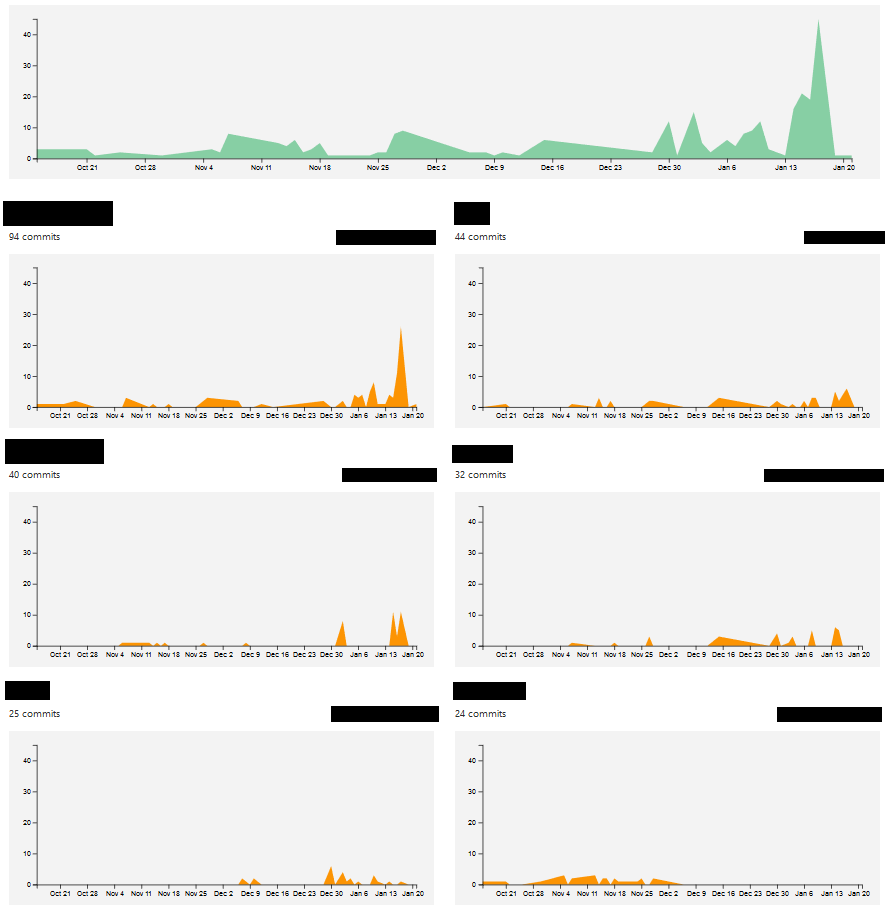
\includegraphics[scale=0.4]{slike/aktivnost.PNG} %veličina slike u odnosu na originalnu datoteku i pozicija slike
			\centering
			\caption{Primjer slike s potpisom}
			\label{fig:promjene}
		\end{figure}
		
		\begin{figure}[H]
			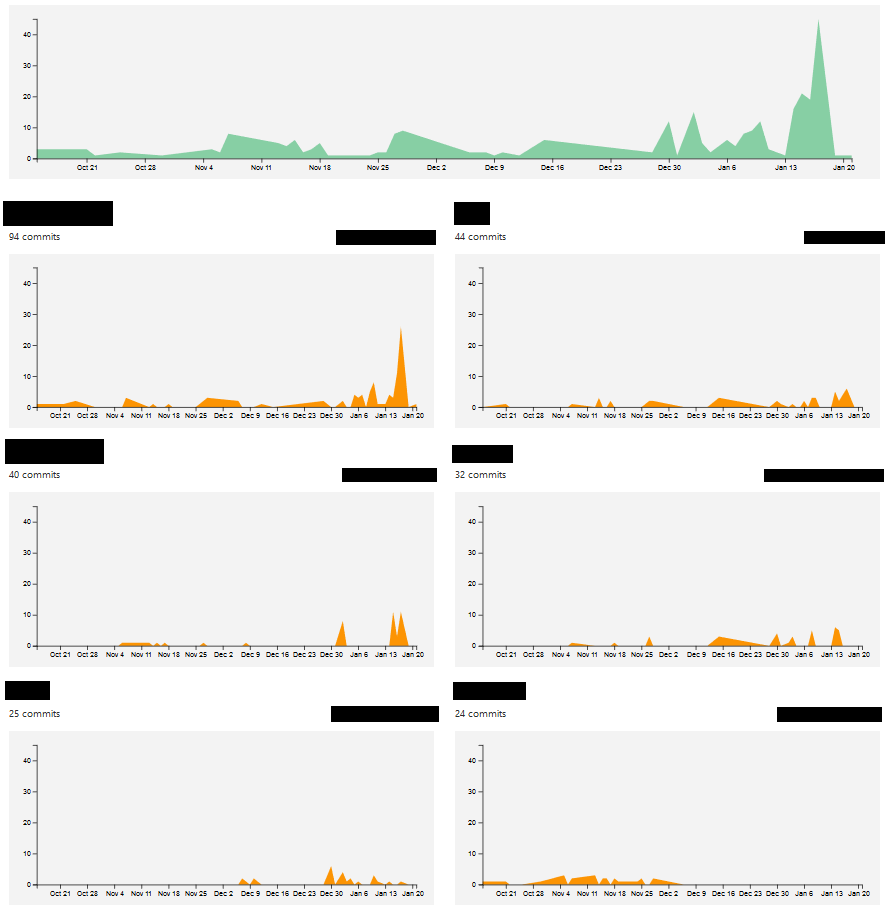
\includegraphics[width=\textwidth]{slike/aktivnost.PNG} %veličina u odnosu na širinu linije
			\caption{Primjer slike s potpisom 2}
			\label{fig:promjene2} %label mora biti drugaciji za svaku sliku
		\end{figure}
		
		Referenciranje slike \ref{fig:promjene2} u tekstu.
		
		\eject
		
	
	\chapter{Specifikacija programske potpore}
		
	\section{Funkcionalni zahtjevi}
			
			\noindent \textbf{Dionici:}
			
			\begin{packed_enum}
				
				\item Vlasnik/naručitelj
				\item Voditelji
				\item Natjecatelji				
				\item Administrator
				\item Razvojni tim
				
			\end{packed_enum}
			
			\noindent \textbf{Aktori i njihovi funkcionalni zahtjevi:}
			
			
			\begin{packed_enum}
				\item  \underbar{Neregistrirani/neprijavljeni korisnik (inicijator) može:}
				
				\begin{packed_enum}
					
					\item vidjeti kalendar s budućim natjecanjima
					\item pregledati dostupne zadatke na stranici
					\item pregledati profile natjecatelja i voditelja
					\item registrirati se u sustav stvaranjem novog korisničkog računa pri čemu odabire jednu od uloga (natjecatelj ili voditelj), a potrebni su mu: korisničko ime, fotografija, lozinka, ime, prezime te email adresa
					
				\end{packed_enum}
			
				\item  \underbar{Natjecatelj (inicijator) može:}
				
				\begin{packed_enum}
					
					\item sudjelovati na natjecanju
					\item vidjeti rang listu natjecatelja na natjecanju kojeg je i sam bio sudionik
					\item vidjeti popis svih učitanih rješenja od ostalih sudionika za prethodno završena natjecanja
					\item pristupiti rješavanju već objavljenih zadataka
					\item izraditi virtualno natjecanje odabirom nekog prošlog natjecanja ili nasumičnim generiranjem zadataka 
					\item vidjeti vlastiti profil s osobnim podacima, statistikom o broju točno riješenih zadatka, broju isprobanih zadataka te prikaz pehara za osvojena natjecanja
					
				\end{packed_enum}
				
				\item  \underbar{Aktivni natjecatelj (inicijator) može:}
				
				\begin{packed_enum}
					
					\item rješavati zadatke i slati datoteke s programskim kodom tijekom natjecanja na kojem se natječe 
					\item osvojiti bodove na natjecanju s obzirom na potrošeno vrijeme za rješavanje zadatka i postotak točnih primjera 
					\item na temelju postignuća za prva tri mjesta osvojiti pehar koji je vidljiv na vlastitom profilu
					
				\end{packed_enum}
				
				\item  \underbar{Voditelj (inicijator) može:}
				
				\begin{packed_enum}
					
					\item pregledati dostupne zadatke na stranici
					\item izraditi novi zadatak pri čemu treba definirati: naziv zadatka, broj bodova, vremensko ograničenje, tekst zadatka i primjere za evaluaciju
					\item organizirati novo natjecanje pri čemu treba definirati: vrijeme početka i završetka, broj zadataka, koji zadaci će biti aktivni te po želji sličicu pehara
					\item uređivati vlastite prethodno objavljene zadatke te natjecanja
					\item vidjeti vlastiti profil s osobnim podacima, popisom učitanih zadataka s mogućnošću sortiranja te kalendar s popisom objavljenih natjecanja
										
				\end{packed_enum}
				
				\item  \underbar{Administrator (inicijator) može:}
				
				\begin{packed_enum}
					
					\item uređivati sve zadatke i natjecanja
					\item potvrditi voditelja prilikom registracije
					\item vidjeti popis svih registriranih korisnika i njihovih osobnih podataka
					\item mijenjati dodijeljena prava i osobne podatke

				\end{packed_enum}
				
				\item  \underbar{Baza podataka (sudionik):}
				
				\begin{packed_enum}
					
					\item pohranjuje sve podatke o korisnicima i njihovim ovlastima te zadacima i natjecanjima
					\item pohranjuje rezultate natjecanja, rješenja zadataka i statistiku natjecatelja			
					
				\end{packed_enum}
			\end{packed_enum}
			
			\eject 
			
			
				
			\subsection{Obrasci uporabe}
				
%				\textbf{\textit{dio 1. revizije}}
%				
%				\subsubsection{Opis obrazaca uporabe}
%					\textit{Funkcionalne zahtjeve razraditi u obliku obrazaca uporabe. Svaki obrazac je potrebno razraditi prema donjem predlošku. Ukoliko u nekom koraku može doći do odstupanja, potrebno je to odstupanje opisati i po mogućnosti ponuditi rješenje kojim bi se tijek obrasca vratio na osnovni tijek.}\\
					

%					\noindent \underbar{\textbf{UC$<$broj obrasca$>$ -$<$ime obrasca$>$}}
%					\begin{packed_item}
%	
%						\item \textbf{Glavni sudionik: }$<$sudionik$>$
%						\item  \textbf{Cilj:} $<$cilj$>$
%						\item  \textbf{Sudionici:} $<$sudionici$>$
%						\item  \textbf{Preduvjet:} $<$preduvjet$>$
%						\item  \textbf{Opis osnovnog tijeka:}
%						
%						\item[] \begin{packed_enum}
%	
%							\item $<$opis korak jedan$>$
%							\item $<$opis korak dva$>$
%							\item $<$opis korak tri$>$
%							\item $<$opis korak četiri$>$
%							\item $<$opis korak pet$>$
%						\end{packed_enum}
%						
%						\item  \textbf{Opis mogućih odstupanja:}
%						
%						\item[] \begin{packed_item}
%	
%							\item[2.a] $<$opis mogućeg scenarija odstupanja u koraku 2$>$
%							\item[] \begin{packed_enum}
%								
%								\item $<$opis rješenja mogućeg scenarija korak 1$>$
%								\item $<$opis rješenja mogućeg scenarija korak 2$>$
%								
%							\end{packed_enum}
%							\item[2.b] $<$opis mogućeg scenarija odstupanja u koraku 2$>$
%							\item[3.a] $<$opis mogućeg scenarija odstupanja  u koraku 3$>$
%							
%						\end{packed_item}
%					\end{packed_item}
					
					\noindent \underbar{\textbf{UC1 - Pregled kalendara}}
					\begin{packed_item}
						
						\item \textbf{Glavni sudionik: } Klijent
						\item \textbf{Cilj:} Pregledati kalendar s nadolazećim natjecanjima 
						\item \textbf{Sudionici:} baza podataka
						\item \textbf{Preduvjet:} -
						\item \textbf{Opis osnovnog tijeka:}
						
						\item[] \begin{packed_enum}
							\item Klijent otvara početnu stranicu web aplikacije
							\item Prikazuje se kalendar
							\item Klijent odabire određeni datum
							\item Aplikacija prikazuje popis nadolazećih natjecanja za odabrani datum
							\item Klijent odabire natjecanje
							\item Prikazuju se detalji i informacije o odabranom natjecanju
						\end{packed_enum}
					\end{packed_item}
					
					
					\noindent \underbar{\textbf{UC2 - Pregled zadataka}}
					\begin{packed_item}
						
						\item \textbf{Glavni sudionik: }Klijent
						\item \textbf{Cilj:} Pregledati zadatke završenih natjecanja
						\item \textbf{Sudionici:} baza podataka
						\item \textbf{Preduvjet:} -
						\item \textbf{Opis osnovnog tijeka:}
						
						\item[] \begin{packed_enum}
							\item Klijent odabire završeno natjecanja
							\item Prikazuje se lista zadatka povezana s odabranim natjecanjem
							\item Klijent odabire specifičan zadatak
							\item Aplikacija prikazuje detalje zadatka
						\end{packed_enum}
					\end{packed_item}
					
					
					\noindent \underbar{\textbf{UC3 - Pregled profila natjecatelja i voditelja}}
					\begin{packed_item}
						
						\item \textbf{Glavni sudionik: }Klijent
						\item \textbf{Cilj:} Pregledati profile natjecatelja i voditelja
						\item \textbf{Sudionici:} baza podataka
						\item \textbf{Preduvjet:} -
						\item \textbf{Opis osnovnog tijeka:}
						
						\item[] \begin{packed_enum}
							\item Klijent otvara profil određenog korisnika klikom na njihovo korisničko ime
							\item Ako je otvoren profil natjecatelja, aplikacija prikazuje informacije o broju točno riješenih zadataka, broju isprobanih zadataka te osvojene pehare
							\item Ako je otvoren profil voditelja, aplikacija prikazuje popis učitanih zadataka i kalendar s popisom objavljenih natjecanja
						\end{packed_enum}
					\end{packed_item}
					
					
					
					\noindent \underbar{\textbf{UC4 - Registracija}}
					\begin{packed_item}
						
						\item \textbf{Glavni sudionik: }Neregistrirani korisnik
						\item  \textbf{Cilj:} Stvoriti korisnički račun
						\item  \textbf{Sudionici:} baza podataka, administrator 
						\item  \textbf{Preduvjet:} korisnik nije prethodno registriran ili prijavljen u sustav
						\item  \textbf{Opis osnovnog tijeka:}
						
						\item[] \begin{packed_enum}
							
							\item Neregistrirani korisnik odabire opciju za registraciju 
							\item Neregistrirani korisnik popunjava obrazac za registraciju s potrebnim podacima 
							\item Neregistrirani korisnik na svoju e-mail adresu prima obavijest i zahtjev za potvrdu registracije
							\item Ako je odabrana uloga "voditelj", sustav dodatno šalje obavijest administratoru 
							\item Administrator potvrđuje registraciju voditelja 
						\end{packed_enum}
						
						\item  \textbf{Opis mogućih odstupanja:}
						\item[] \begin{packed_item}
							
							\item[2.a] Već zauzeto korisničko ime ili e-mail adresa, uneseni podaci u nedozvoljenom formatu ili neispravna e-mail adresa 
							\item[] \begin{packed_enum}
								
								\item Sustav obavještava korisnika o neuspjelom unosu i prikazuje relevantne poruke o greškama 
								\item Korisnik mijenja potrebne podatke te završava unos ili odustaje od registracije 
								
							\end{packed_enum}
							
							\item[5.a] Administrator odbija zahtjev za registraciju voditelja natjecanja:
							\item[] \begin{packed_enum}
								
								\item Sustav obavještava korisnika putem e-maila
								
							\end{packed_enum}
						\end{packed_item}
					\end{packed_item}
					
					\noindent \underbar{\textbf{UC5 - Prijava}}
					\begin{packed_item}
						
						\item \textbf{Glavni sudionik: }Neprijavljeni korisnik
						\item \textbf{Cilj:} Dobiti pristup korisničkom sučelju
						\item \textbf{Sudionici:} baza podataka
						\item \textbf{Preduvjet:} korisnik je registriran u sustav, ali nije prijavljen
						\item \textbf{Opis osnovnog tijeka:}
						\item[] \begin{packed_enum}
							\item Korisnik unosi korisničko ime i lozinku
							\item Sustav potvrđuje ispravnosti unesenih podataka
							\item Korisniku je omogućen pristup korisničkim funkcijama
						\end{packed_enum}
						
						\item  \textbf{Opis mogućih odstupanja:}
						
						\item[] \begin{packed_item}
							
							\item[2.a] Neispravno korisničko ime/lozinka
							\item[] \begin{packed_enum}
								
								\item Sustav obavještava korisnika o neuspjeloj prijavi uz informaciju o pogrešci i omogućuje korisniku ponovan pokušaj prijave
								
							\end{packed_enum}
						\end{packed_item}
					\end{packed_item}
					
					\noindent \underbar{\textbf{UC6 - Pregled profila}}
					\begin{packed_item}
						
						\item \textbf{Glavni sudionik: }Prijavljeni korisnik
						\item \textbf{Cilj:} Pregledati vlastiti profil
						\item \textbf{Sudionici:} baza podataka
						\item \textbf{Preduvjet:} korisnik je prijavljen
						\item \textbf{Opis osnovnog tijeka:}
						\item[] \begin{packed_enum}
							\item Prijavljeni korisnik pristupa opciji "Moj profil" klikom na ikonu profila
							\item Aplikacija prikazuje podatke o prijavljenom korisniku (ime, fotografija, lozinka, ime, prezime i e-mail adresa)
						\end{packed_enum}
					\end{packed_item}
					
					
					
					\noindent \underbar{\textbf{UC7 - Pregled vlastite statistike}}
					\begin{packed_item}
						
						\item \textbf{Glavni sudionik: }Natjecatelj
						\item \textbf{Cilj:} Pregledati vlastitu statistiku unutar web aplikacije
						\item \textbf{Sudionici:} baza podataka
						\item \textbf{Preduvjet:} korisnik je prijavljen
						\item \textbf{Opis osnovnog tijeka:}
						
						\item[] \begin{packed_enum}
							\item Korisnik pristupa svojem profilu i odabire opciju "Moje statistike"
							\item Aplikacija prikazuje statistike korisnika(broj točno riješenih zadataka, broj isprobanih zadataka, pehare za osvojena natjecanja)
						\end{packed_enum}
					\end{packed_item}

					
					\noindent \underbar{\textbf{UC8 - Pregled vlastitih zadataka}}
					\begin{packed_item}
						
						\item \textbf{Glavni sudionik: }Voditelj
						\item \textbf{Cilj:} Pregledati popis svih vlastito objavljenih zadataka
						\item \textbf{Sudionici:} baza podataka
						\item \textbf{Preduvjet:} korisnik je prijavljen
						\item \textbf{Opis osnovnog tijeka:}
						
						\item[] \begin{packed_enum}
							\item Voditelj odabire opciju za prikaz vlastitih zadataka
							\item Prikazuju se svi objavljeni zadaci tog voditelja
						\end{packed_enum}
					\end{packed_item}
										
										
										
					\noindent \underbar{\textbf{UC9 – Sudjelovanje na natjecanju}}
					\begin{packed_item}
						
						\item \textbf{Glavni sudionik: }Natjecatelj
						\item \textbf{Cilj:} Pristupiti natjecanju 
						\item \textbf{Sudionici:} baza podataka
						\item \textbf{Preduvjet:} korisnik je prijavljen i postoji natjecanje u tijeku
						\item \textbf{Opis osnovnog tijeka:}
						
						\item[] \begin{packed_enum}
							\item Prikazuju se informacije o natjecanju u tijeku i natjecatelj potvrđuje da želi sudjelovati na natjecanju 
							\item Natjecatelju se prikazuju zadaci koji su dio natjecanja te preostalo vrijeme do kraja natjecanja
						\end{packed_enum}
					\end{packed_item}
								
					
					
					\noindent \underbar{\textbf{UC10 – Prijenos datoteke rješenja}}
					\begin{packed_item}
						
						\item \textbf{Glavni sudionik: }Natjecatelj, Aktivni natjecatelj
						\item \textbf{Cilj:} Prenijeti datoteku kao rješenje nekog zadatka na natjecanju
						\item \textbf{Sudionici:} baza podataka
						\item \textbf{Preduvjet:} natjecatelj je pristupio natjecanju ili rješavanju zadataka
						\item \textbf{Opis osnovnog tijeka:}
						
						\item[] \begin{packed_enum}
							\item Korisnik nakon napisanog rješenja zadatka odabire opciju za predaju rješenja
							\item Korisnik odabire datoteku s rješenjem koju želi predati i potvrđuje odabir
							\item Datoteka se prenosi, predaje kao rješenje i šalje na evaluaciju
						\end{packed_enum}
						
							\item  \textbf{Opis mogućih odstupanja:}
							
							\item[] \begin{packed_item}
								
								\item[2.a] Odabir pogrešne datoteke
								\item[] \begin{packed_enum}
									
									\item Aktivni natjecatelj odabire opciju za brisanje datoteke 
									\item Aktivni natjecatelj ponovno kreće s 1. korakom iz osnovnog tijeka
																
								\end{packed_enum}
							\end{packed_item}
						\end{packed_item}
									
									
					
					\noindent \underbar{\textbf{UC11 – Pregled rang liste}}
					\begin{packed_item}
						
						\item \textbf{Glavni sudionik: }Natjecatelj
						\item \textbf{Cilj:} Pregledati rang listu nekog natjecanja
						\item \textbf{Sudionici:} baza podataka
						\item \textbf{Preduvjet:} korisnik je prijavljen kao natjecatelj
						\item \textbf{Opis osnovnog tijeka:}
						
						\item[] \begin{packed_enum}
							\item Natjecatelj odabire opciju za prikaz prošlih natjecanja na kojima je sudjelovao
							\item Odabire natjecanje za koje želi vidjeti rang listu ostalih sudionika i odabire prikaz rang liste
							\item Otvara se popis s prikazom postignuća ostalih sudionika po broju ostvarenih bodova
						\end{packed_enum}
					\end{packed_item}
										
										
					\noindent \underbar{\textbf{UC12 – Pregled rješenja zadataka}}
					\begin{packed_item}
						
						\item \textbf{Glavni sudionik: }Natjecatelj
						\item \textbf{Cilj:} Vidjeti tuđa rješenja zadataka s nekog natjecanja
						\item \textbf{Sudionici:} Baza podataka
						\item \textbf{Preduvjet:} Natjecatelj je sudjelovao na natjecanju koje je završilo
						\item \textbf{Opis osnovnog tijeka:}
						
						\item[] \begin{packed_enum}
							\item Natjecatelj odabire opciju za prikaz prošlih natjecanja na kojima je sudjelovao
							\item Natjecatelj odabire natjecanje za koje želi vidjeti predana rješenja 
							\item Prikazuju se informacije o natjecanju s popisom svih predanih rješenja
							\item Odabirom opcije za prikaz natjecanja po zadacima prikazuje se pregled zadataka s tog natjecanja
							\item Odabirom zadatka otvara se tekst zadatka s prikazom svih predanih rješenja drugih sudionika uz informacije o uspješnosti predanog rješenja
						\end{packed_enum}
					\end{packed_item}
										
										
										
					\noindent \underbar{\textbf{UC13 – Rješavanje zadataka}}
					\begin{packed_item}
						
						\item \textbf{Glavni sudionik: }Natjecatelj
						\item \textbf{Cilj:} Vježbanje već objavljenih zadataka
						\item \textbf{Sudionici:} baza podataka
						\item \textbf{Preduvjet:} korisnik je prijavljen kao natjecatelj
						\item \textbf{Opis osnovnog tijeka:}
						
						\item[] \begin{packed_enum}
							\item Natjecatelj odabire opciju za prikaz svih objavljenih zadataka
							\item Prikazuje se popis svih zadataka
							\item Odabirom zadatka koji želi rješavati otvara se sučelje slično onom na natjecanju koje natjecatelju omogućuje učitavanje datoteke kao rješenja zadataka i evaluiranje istog
						\end{packed_enum}
					\end{packed_item}
									
								
					
					\noindent \underbar{\textbf{UC14 – Izrada virtualnog natjecanja}}
					\begin{packed_item}
						
						\item \textbf{Glavni sudionik: }Natjecatelj
						\item \textbf{Cilj:} Vježbanje simuliranjem pravog natjecanja
						\item \textbf{Sudionici:} baza podataka
						\item \textbf{Preduvjet:} postoji barem jedno završeno natjecanje i/ili barem jedan javno vidljiv zadatak u bazi
						\item \textbf{Opis osnovnog tijeka:}
						
						\item[] \begin{packed_enum}
							\item Natjecatelj odabire opciju “virtualno natjecanje”
							\item Otvara se prikaz s dvije mogućnosti odabira
							\item Natjecatelj odabire jednu od dvije opcije - stvaranje natjecanja pokretanjem nekog prošlog natjecanja iz kalendara ili stvaranje natjecanja nasumičnim odabirom zadataka iz baze zadataka
							\item Natjecanje se stvara i natjecatelj može krenuti s rješavanjem zadataka
						\end{packed_enum}
					\end{packed_item}
										
										
										
					\noindent \underbar{\textbf{UC15 – Unos novog zadatka}}
					\begin{packed_item}
						
						\item \textbf{Glavni sudionik: }Voditelj
						\item \textbf{Cilj:} Stvoriti novi zadatak u bazi postojećih zadataka
						\item \textbf{Sudionici:} baza podataka
						\item \textbf{Preduvjet:} korisnik je prijavljen kao voditelj
						\item \textbf{Opis osnovnog tijeka:}
						
						\item[] \begin{packed_enum}
							\item Voditelj odabire opciju za unos novog zadatka
							\item Otvara se forma gdje voditelj upisuje potrebne podatke
							\item Voditelj odabire želi li zadatak stvoriti kao privatan ili javan
							\item Voditelj potvrđuje unos zadatka
							\item Zadatak se pohranjuje u bazu ostalih zadataka s informacijom o autoru zadatka
						\end{packed_enum}
						
						\item  \textbf{Opis mogućih odstupanja:}
						\item[] \begin{packed_item}
							
							\item[2.a] Voditelj ostavlja prazno neko polje u formi i pokušava predati takav zadatak
							\item[] \begin{packed_enum}
								
								\item Sustav ga obavještava o neispravnom pokušaju predaje zadatka 
								\item Sustav omogućuje ponovno ispunjavanje forme u svrhu ispravne predaje
								
							\end{packed_enum}
						\end{packed_item}
					\end{packed_item}
					
					\noindent \underbar{\textbf{UC16 – Uređivanje zadatka}}
					\begin{packed_item}
						
						\item \textbf{Glavni sudionik: }Voditelj
						\item \textbf{Cilj:} Uređivanje postojećeg zadatka
						\item \textbf{Sudionici:} baza podataka
						\item \textbf{Preduvjet:} postoji zadatak koji je prijavljeni voditelj unio u bazu
						\item \textbf{Opis osnovnog tijeka:}
						
						\item[] \begin{packed_enum}
							\item Voditelj odabire opciju “moji zadaci”
							\item Otvara se pregled svih zadataka koje je voditelj unio u sustav
							\item Voditelj odabire opciju uređivanja zadataka
							\item Otvara se forma slična onoj kod unosa novog zadatka koja voditelju omogućuje izmjenu podataka te spremanje istih
						\end{packed_enum}
					\end{packed_item}
					
					
					
					\noindent \underbar{\textbf{UC17 – Organiziranje natjecanja}}
					\begin{packed_item}
						
						\item \textbf{Glavni sudionik: }Voditelj
						\item \textbf{Cilj:} Organizirati novo natjecanje
						\item \textbf{Sudionici:} baza podataka
						\item \textbf{Preduvjet:} korisnik je prijavljen
						\item \textbf{Opis osnovnog tijeka:}
						
						\item[] \begin{packed_enum}
							\item Voditelj odabire opciju za organiziranje novog natjecanja
							\item Otvara se forma gdje voditelj odabire vrijeme početka i završetka natjecanja, broj zadataka, koji zadaci će biti aktivni te po želji učitava sličicu pehara
							\item Voditelj potvrđuje podatke o novom natjecanju
							\item Natjecanje se dodaje u kalendar natjecanja
							
						\end{packed_enum}
						
						\item  \textbf{Opis mogućih odstupanja:}
						\item[] \begin{packed_item}
							
							\item[2.a] Voditelj ne ispunjava neko polje u formi i pokušava potvrditi natjecanje
							\item[] \begin{packed_enum}
								
								\item Sustav ga obavještava o neispravnosti ispunjene forme
								\item Sustav omogućuje ponovno ispunjavanje forme u svrhu ispravne predaje
								
							\end{packed_enum}
						\end{packed_item}
					\end{packed_item}
										
					\noindent \underbar{\textbf{UC18 – Uređivanje natjecanja}}
					\begin{packed_item}
						
						\item \textbf{Glavni sudionik: }Voditelj
						\item \textbf{Cilj:} Uređivanje postojećeg natjecanja
						\item \textbf{Sudionici:} baza podataka
						\item \textbf{Preduvjet:} postoji natjecanje koje je prijavljeni voditelj organizirao, a ono nije u tijeku ili završeno
						\item \textbf{Opis osnovnog tijeka:}
						
						\item[] \begin{packed_enum}
							\item Voditelj odabire opciju “moja natjecanja”
							\item Otvara se pregled svih natjecanja koje je voditelj organizirao
							\item Voditelj odabire opciju uređivanja natjecanja kojemu želi izmijeniti podatke
							\item Otvara se pregled sličan onom prilikom organiziranja novog natjecanja koji voditelju omogućuje izmjenu i spremanje novih postavki natjecanja
						\end{packed_enum}
					\end{packed_item}
					
					\noindent \underbar{\textbf{UC19 – Pregled svih korisnika u bazi}}
					\begin{packed_item}
						
						\item \textbf{Glavni sudionik: }Administrator
						\item \textbf{Cilj:} Pregled svih registriranih korisnika u bazi
						\item \textbf{Sudionici:} baza podataka
						\item \textbf{Preduvjet:} -
						\item \textbf{Opis osnovnog tijeka:}
						
						\item[] \begin{packed_enum}
							\item Administrator odabire opciju prikaza korisnika u bazi
							\item Otvara se popis svih registriranih BytePit korisnika
							
						\end{packed_enum}
					\end{packed_item}
					
					
					
					\noindent \underbar{\textbf{UC20 – Izmjena osobnih podataka}}
					\begin{packed_item}
						
						\item \textbf{Glavni sudionik: }Administrator
						\item \textbf{Cilj:} Uređivanje podataka nekog korisnika
						\item \textbf{Sudionici:} baza podataka
						\item \textbf{Preduvjet:} postoji barem jedan registrirani korisnik u bazi 
						\item \textbf{Opis osnovnog tijeka:}
						
						\item[] \begin{packed_enum}
							\item Administrator odabire opciju prikaza korisnika u bazi
							\item Otvara se popis svih registriranih BytePit korisnika
							\item Odabirom korisnika prikazuju se njegovi osobni podaci s mogućnošću izmjene istih uključujući i izmjenu dodijeljene uloge korisniku
							
						\end{packed_enum}
					\end{packed_item}
					
					
					\noindent \underbar{\textbf{UC21 – Brisanje korisnika}}
					\begin{packed_item}
						
						\item \textbf{Glavni sudionik: }Administrator
						\item \textbf{Cilj:} Brisanje postojećeg korisnika iz baze podataka
						\item \textbf{Sudionici:} baza podataka
						\item \textbf{Preduvjet:} postoji barem jedan registrirani korisnik u bazi
						\item \textbf{Opis osnovnog tijeka:}
						
						\item[] \begin{packed_enum}
							\item Administrator odabire opciju prikaza korisnika u bazi
							\item Otvara se popis svih registriranih BytePit korisnika
							\item Administrator odabire i potvrđuje opciju brisanja korisnika 
							\item Korisnik se briše iz baze podataka
							
						\end{packed_enum}
					\end{packed_item}
					
				
					
				\subsubsection{Dijagrami obrazaca uporabe}
					
					\begin{figure}[H]
						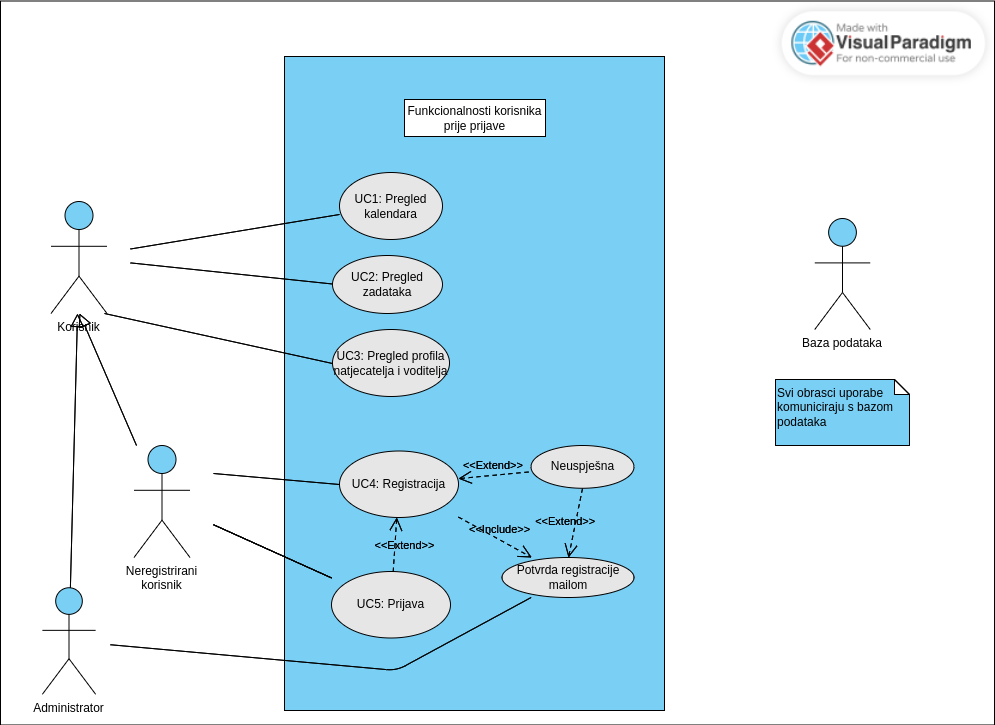
\includegraphics[scale=0.4]{dijagrami/obrasci_uporabe1.png} 
						\centering
						\caption{Obrasci uporabe - funkcionalnosti za neprijavljene korisnike}
						\label{fig:obrasci_uporabe1}
					\end{figure}
					
					\begin{figure}[H]
						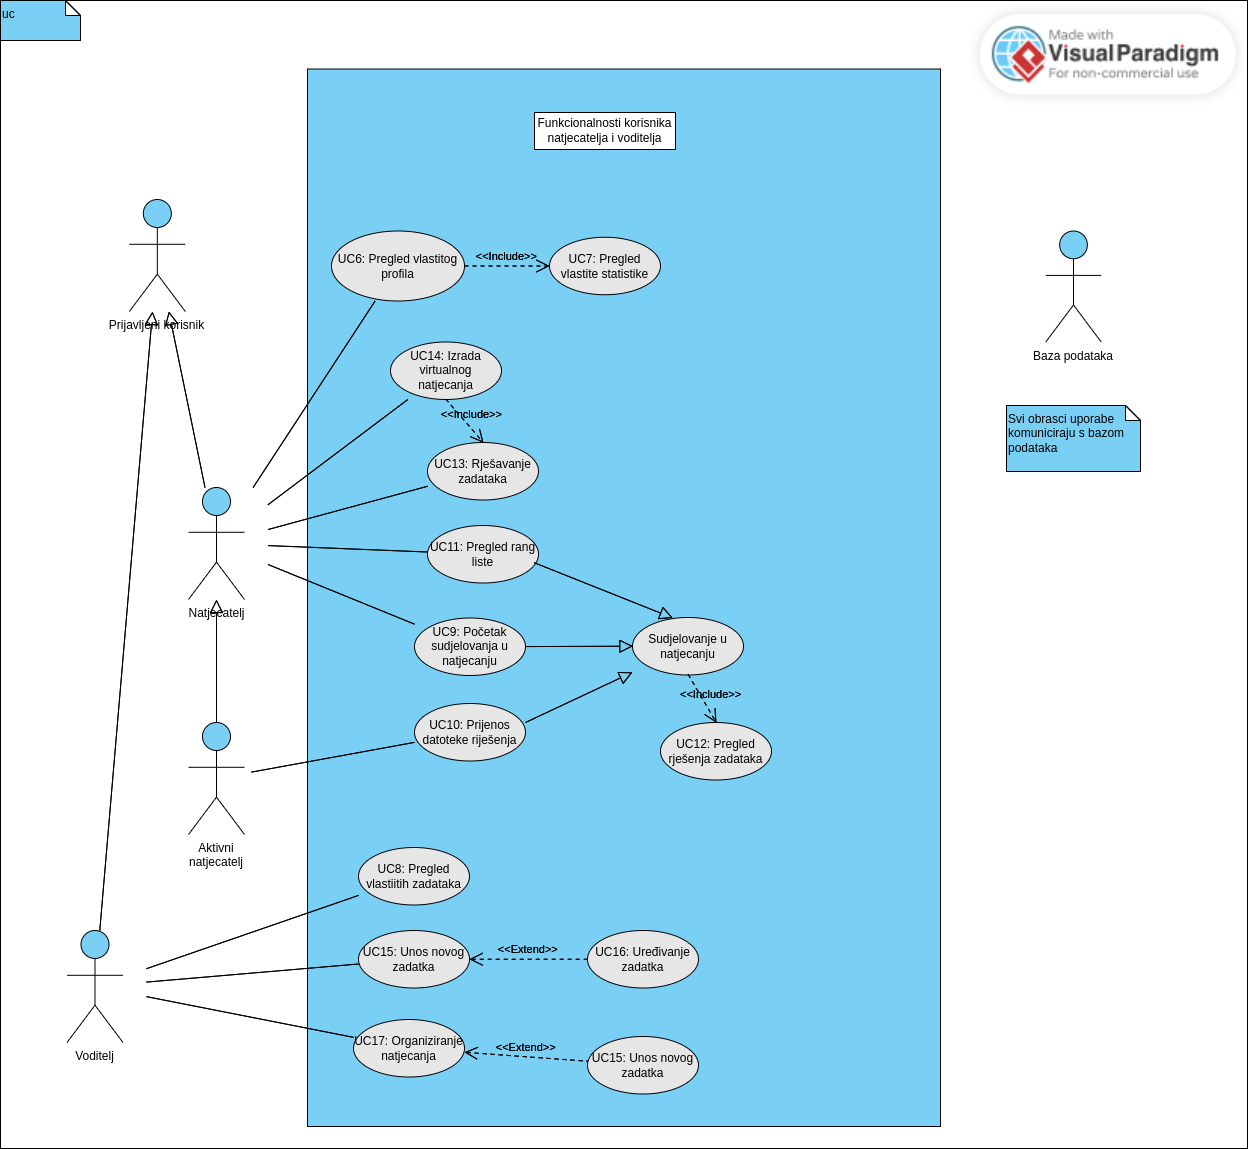
\includegraphics[scale=0.4]{dijagrami/obrasci_uporabe2.png} 
						\centering
						\caption{Obrasci uporabe - funkcionalnosti za natjecatelje i voditelje}
						\label{fig:obrasci_uporabe2}
					\end{figure}
					
					\begin{figure}[H]
						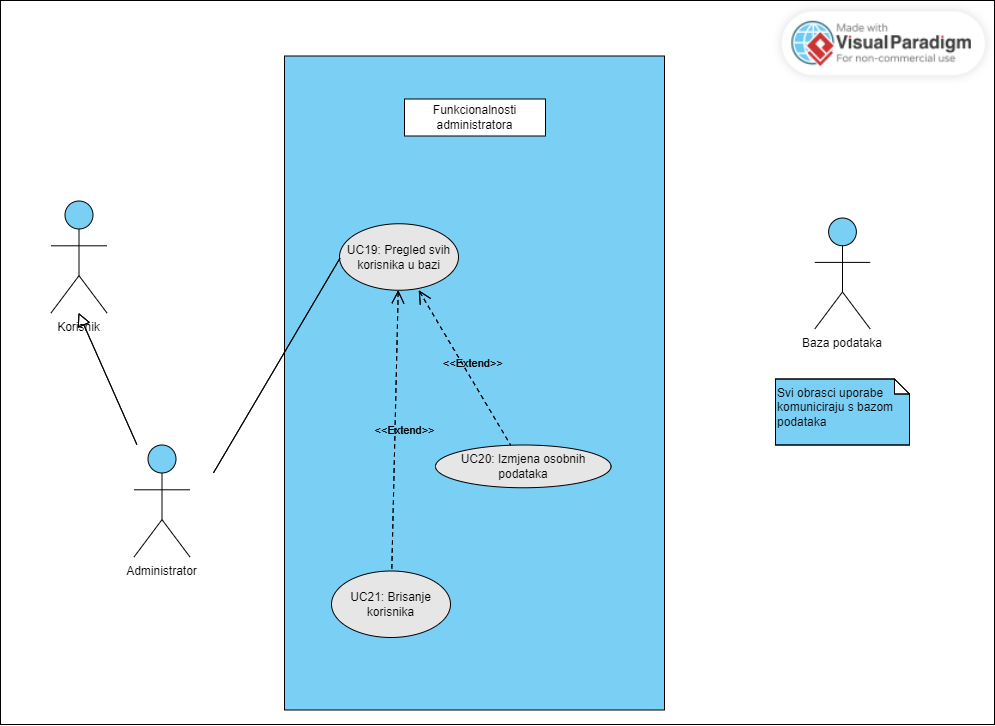
\includegraphics[scale=0.4]{dijagrami/obrasci_uporabe3.png} 
						\centering
						\caption{Obrasci uporabe - funkcionalnosti za administratore}
						\label{fig:obrasci_uporabe3}
					\end{figure}
				\eject		
				
			\subsection{Sekvencijski dijagrami}
				
%				\textbf{\textit{dio 1. revizije}}\\
%				
%				\textit{Nacrtati sekvencijske dijagrame koji modeliraju najvažnije dijelove sustava (max. 4 dijagrama). Ukoliko postoji nedoumica oko odabira, razjasniti s asistentom. Uz svaki dijagram napisati detaljni opis dijagrama.}


				\noindent \textbf{UC15 – unos novog zadatka}\\
				
				\noindent Korisnik prijavljen u sustav kao voditelj odabire opciju za stvaranje novog zadatka. Poslužitelj prikazuje formu s praznim poljima koje voditelj treba ispuniti podacima o zadatku. Točnije, potrebno je navesti naziv zadatka, broj bodova koje nosi, vremensko ograničenje izvršavanja, tekst zadatka i primjere za evaluaciju, a moguće je i odabrati opciju da zadatak bude stvoren kao privatan. Voditelj upisuje navedene podatke te ih šalje poslužitelju koji prvo provjerava da su svi podaci ispravno uneseni te da nema polja koja su ostala prazna. U slučaju neispravnosti podataka, poslužitelj prikazuje relevantnu poruku o problemu i ponovno omogućuje ispunjavanje forme. Nakon uspješne provjere, podaci se šalju bazi podataka koja ih sprema i time stvara novi zadatak. Ako sve prođe bez problema, baza podataka šalje potvrdu poslužitelju o uspješnom stvaranju novog zadatka, a poslužitelj zatim javlja korisniku da je njegov zahtjev uspješno proveden.
				
				\begin{figure}[H]
					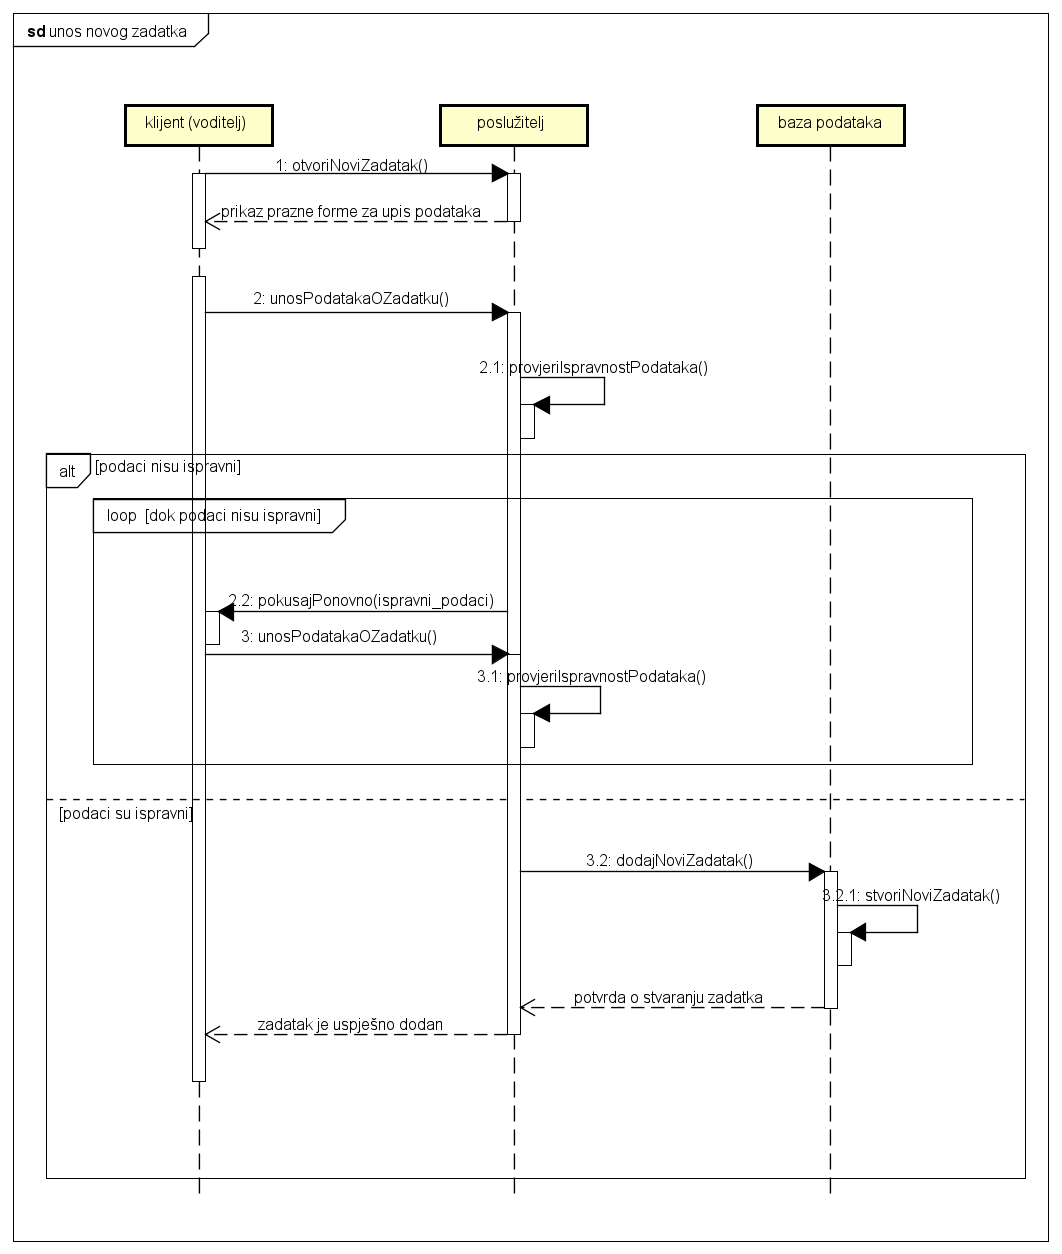
\includegraphics[scale=0.6]{dijagrami/sd15.png} 
					\centering
					\caption{Sekvencijski dijagram za obrazac uporabe - unos novog zadatka}
					\label{fig:sekvencijski1}
				\end{figure}
				\pagebreak
				
				\noindent \textbf{UC17 – organiziranje novog natjecanja}\\
				
				\noindent Korisnik prijavljen u sustav kao voditelj odabire opciju za stvaranjem novog natjecanja. Poslužitelj prikazuje formu s praznim poljima koje je voditelj dužan ispuniti informacijama o natjecanju. Potrebno je unijeti vrijeme početka i završetka natjecanja, broj zadataka, odabrati zadatke koji će biti aktivni te po želji učitati sličicu pehara, koja se pohranjuje u bazu podataka, kojom se nagrađuju najbolji natjecatelji. U slučaju da je voditelj izostavio nešto i ostavio polje praznim, sustav će ga obavijestiti i zatražiti ponovni unos podataka. Nakon uspješno ispunjene forme i uspješno primljenih podataka, poslužitelj će ih proslijediti bazi podataka i zatražiti stvaranje novog natjecanja. Nakon pohrane, ako sve prođe bez problema, baza podataka bi trebala poslati povratnu informaciju poslužitelju o uspješnom stvaranju novog natjecanja, a poslužitelj bi zatim trebao javiti korisniku da je njegov zahtjev uspješno proveden.
				
				\begin{figure}[H]
					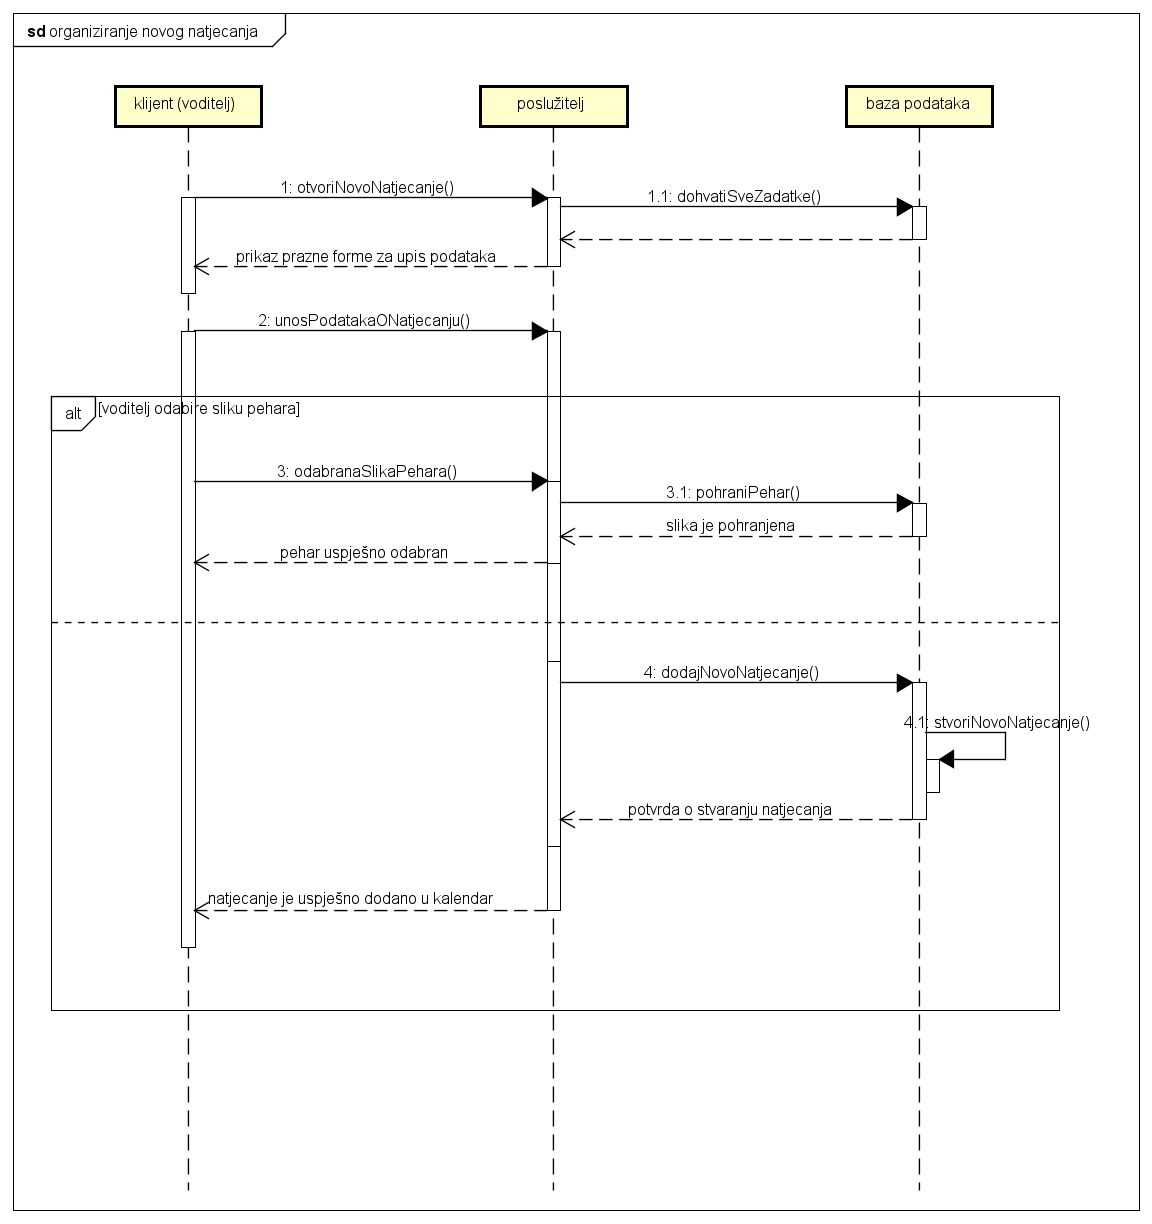
\includegraphics[scale=0.5]{dijagrami/sd17.png} 
					\centering
					\caption{Sekvencijski dijagram za obrazac uporabe - organiziranje novog natjecanja}
					\label{fig:sekvencijski2} 
				\end{figure}
				\pagebreak
				
				\noindent \textbf{UC10 i UC13 – rješavanje zadataka i prijenos datoteke}\\
				
				\noindent Korisnik prijavljen u sustav kao natjecatelj odabire opciju za prikaz svih objavljenih zadataka. Poslužitelj prikazuje popis svih javnih zadataka. Natjecatelj zatim bira zadatak koji želi pokušati riješiti pri čemu se otvara sučelje s tekstom zadatka i opcijom za prijenos datoteke rješenja. Natjecatelj odabire datoteku koju želi prenijeti kao rješenje i potvrđuje svoj odabir, a poslužitelj prosljeđuje datoteku do baze podataka koja ju sprema za prikaz prilikom nekih drugih funkcionalnosti. Na klijentov zahtjev predana datoteka se predaje evaluatoru koji pomoću definiranih primjera ulaza i izlaza određuje točnost rješenja zadatka i vraća ih poslužitelju. Poslužitelj sve rezultate sprema u bazu podataka i prikazuje klijentu u aplikaciji.
				
				\begin{figure}[H]
					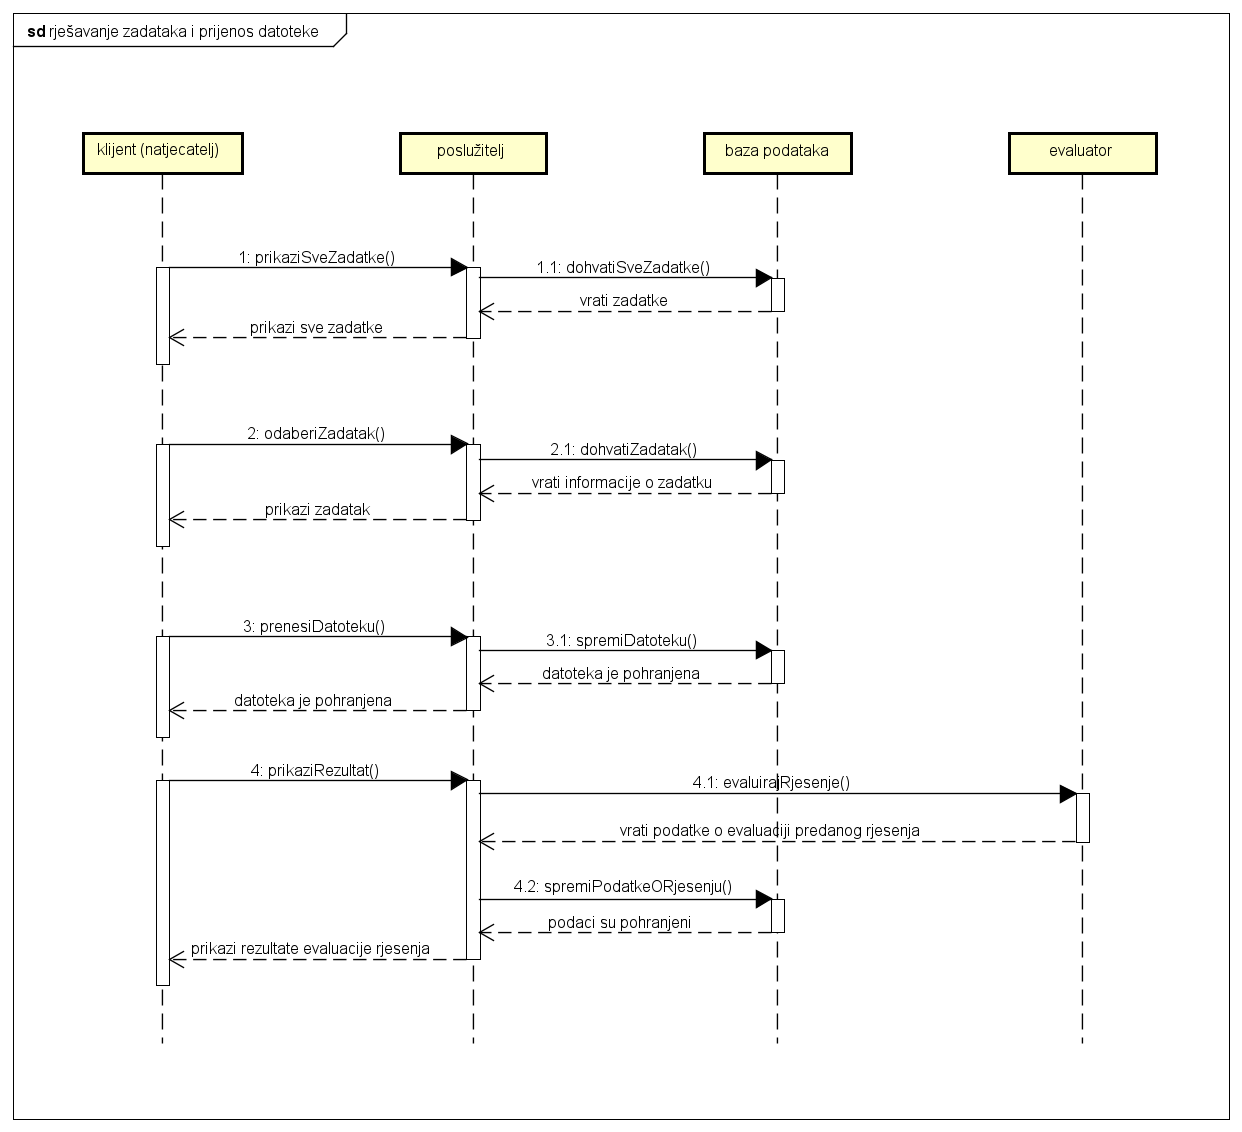
\includegraphics[scale=0.5]{dijagrami/sd10_sd13.png} 
					\centering
					\caption{Sekvencijski dijagram za obrasce uporabe -  rješavanje zadataka i prijenos datoteke}
					\label{fig:sekvencijski3}
				\end{figure}
				

				\eject	
		\section{Ostali zahtjevi}
			 
			 \begin{packed_item}
			 	
			 	\item Sustav treba dopustiti višekorisnički rad u stvarnom vremenu.
			 	\item Sustav treba biti jednostavan i intuitivan za korištenje tako da djeca nemaju problema sa razumijevanjem i snalaženjem na aplikaciji.
			 	\item Sustav se treba izgraditi kao mrežna aplikacija pomoću objektno-orijentiranih jezika.
			 	\item Sustav treba biti prilagođen za hrvatski jezik i abecedu prilikom prikaza i unosa tekstualnog sadržaja, uključujući i dijakritičke znakove.
			 	\item Pristup sustavu treba biti omogućen putem javne mreže.
			 	\item Sustav treba omogućiti evaluaciju rješenja zadataka za minimalno jedan programski jezik.
			 	\item Sustav treba biti takav da se sve funkcije izvršavaju brzo, ne duže od nekoliko sekundi, uključujući i evaluaciju rješenja zadataka.
			 	\item Baza podataka sustava mora biti kvalitetno i ispravno povezana sa sučeljem aplikacije.
			 	
			 \end{packed_item}
			 
	
	\chapter{Arhitektura i dizajn sustava}

\begin{figure}[H]
	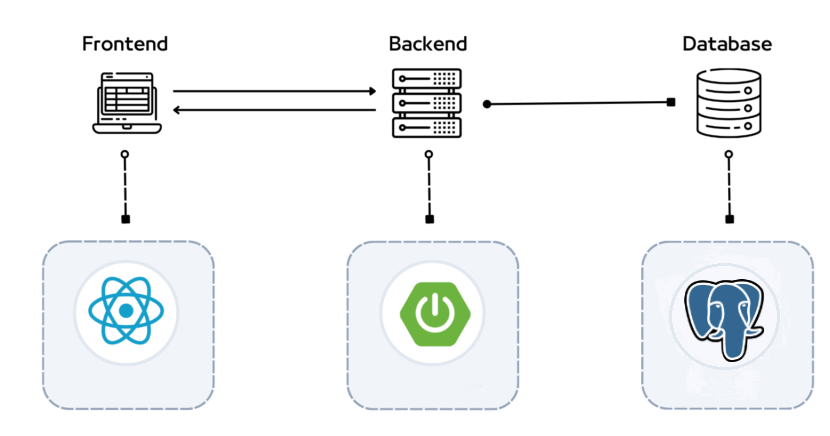
\includegraphics[scale=1]{slike/prikaz_arhitekture.png}
	\centering
	\caption{Prikaz arhitekture sustava}
\end{figure}

Arhitektura sustava može se podijeliti na tri glavna podsustava, a to su \textbf{Frontend Web aplikacija, Backend Web aplikacija i baza podataka}.
\begin{itemize}
	\item 	\textit{\textbf{Web poslužitelj}} prima zahtjeve od klijenata putem interneta, obrađuje ih i pruža resurse poput web stranice, slike, videa i datoteke kao odgovor. Za distribuciju resursa najčešče se koriste protokoli kao što su HTTP (Hypertext Transfer Protocol) ili HTTPS (HTTP Secure).
	\item 	\textit{\textbf{Web aplikacija}} je program koji se izvršava na web pregledniku (Google Chrome, Mozilla Firefox, Safari itd.) i pruža korisnicima mogućnost izvršavanja željenih zahtjeva, odnosno interakciju s određenim uslugama i funkcionalnostima web aplikacije. Prilikom obrade zahtjeva pristupa se bazi podataka i korisniku se odgovor vraća kao HTML dokument.
	\item 	\textit{\textbf{Baza podataka}} je organizirani skup podataka namijenjen za efikasno upravljanje, ažuriranje, pretraživanje i dohvat podataka. Uloge baze podataka u web aplikaciji su pohrana podataka, očuvanje integriteta podataka i osiguravanje dosljednosti, upravljanje transakcijama itd.
\end{itemize}

Za izradu naše web aplikacije odabrali smo \textit{\textbf{Spring Boot}} (open-source Java framework) i \textit{\textbf{React}} (open-source JavaScript library). Odabrana razvojna okruženja su InteliJ IDEA i Eclipse IDE za Spring Boot, odnosno Visual Studio Code i WebStorm za React. Za izradu baze podatka koristimo PostgreSQL.
Arhitektura, koja je podržana Spring Boot-om, temelji se na \textit{\textbf{MVC (Model-View-Controller)}} konceptu koji strogo odvaja model, akcije i prezentaciju, olakšava razvoj i održavanje aplikacije te čini aplikaciju prilagodljivom i jednostavnom za proširenje.
\begin{itemize}
	\item \textit{\textbf{Model}} - predstavlja poslovnu logiku, odnosno dinamičke strukture podataka, mijenja pogled na zahtjev kontrolera. Modeli u pravilu predstavljaju podatke(objekte) koje aplikacija obrađuje.
	\item \textit{\textbf{View}} - ono što klijent vidi, odnosno korisničko sučelje potrebno za interakciju s aplikacijom kao što su dijagrami, linkovi, slike, tablice itd.
	\item \textit{\textbf{Controller}} - presreće zahtjeve klijenata i prilagođava model, odnosno obavještava model o promjeni zahtjeva korisnika i u skladu sa zahtjevima daje prikladan View.
\end{itemize}

\section{Baza podataka}
			
Za potrebe našeg sustava koristit ćemo relacijsku bazu podataka koja svojom strukturom olakšava modeliranje stvarnog svijeta. Gradivna jedinka baze je relacija, od- nosno tablica koja je definirana svojim imenom i skupom atributa. Zadaća baze podataka je brza i jednostavna pohrana, izmjena i dohvat podataka za daljnju obradu. Baza podataka ove aplikacije sastoji se od sljedećih entiteta:
\begin{itemize}
	\item Natjecanje
	\item VirtualnoNatjecanje
	\item Korisnik
	\item Pehar
	\item Zadatak
	\item Rješenje
	\item TestniPrimjer		
\end{itemize}
				
\subsection{Opis tablica}
			

\textbf{Natjecanje} \quad Ovaj entiet sadržava informacije o natjecanju koje trenutno rješava korisnik. Atributi koje sadržava su: NatjecanjeID, VoditeljID, NazivNatjecanja, PocetakNatjecanja, ZavršetakNatjecanja. Ovaj entitet ima  \textit{One-to-Many} vazu s entitetom Pehar preko atributa NatjecanjeID, te  \textit{One-to-Many} vezu sa slabim entitetom VirtualnoNatjecanje preko atributa OriginalnoNajtecanjeID. Ima  \textit{One-to-Many} vezu s entitetom Korisnik preko atributa VoditeljID.
				
				
				\begin{longtblr}[
					label=none,
					entry=none
					]{
						width = \textwidth,
						colspec={|X[9,l]|X[6, l]|X[18, l]|}, 
						rowhead = 1,
					} %definicija širine tablice, širine stupaca, poravnanje i broja redaka naslova tablice
					\hline \SetCell[c=3]{c}{\textbf{Natjecanje}}	 \\ \hline[3pt]
					\SetCell{LightGreen}NatjecanjeID & INT	&  	Jedinstveni identifikator natjecanja  	\\ \hline
					\SetCell{LightBlue}VoditeljID	& INT &  Jedinstveni identifikator voditelja 	\\ \hline 
					NazivNatjecanja & VARCHAR &  Naziv natjecanja \\ \hline 
					PocetakNatjecanja & TIMESTAMP	&  	Vrijeme početka natjecanja	\\ \hline 
					ZavrsetakNatjecanja	& TIMESTAMP &   Vrijeme završetka natjecanja	\\ \hline 
				\end{longtblr}
				
\textbf{VirtualnoNatjecanje} \quad Ovaj enitet sadržava informacije o virtualnom natjecanju koje je pokrenuo korisnik na temelju nekog natjecanja. Atributi koje sadržava su: virtualnoNatjecanjeID, natjecateljID i originalnoNatjecanjeID. Ovaj entitet ima \textit{Many-To-One} vezu s entitetom Korisnik preko atributa i vanjskog ključa korisnikID. Atribut originalnoNatjecanjeID predstavlja vanjski ključ koji se referencira na natjecanjeID u relaciji natjecanje pa se time tvori \textit{Many-To-One} veza.
		
				\begin{longtblr}[
					label=none,
					entry=none
					]{
						width = \textwidth,
						colspec={|X[11,l]|X[3, l]|X[20, l]|}, 
						rowhead = 1,
					} %definicija širine tablice, širine stupaca, poravnanje i broja redaka naslova tablice
					\hline \SetCell[c=3]{c}{\textbf{VirtualnoNatjecanje}}	 \\ \hline[3pt]
					\SetCell{LightGreen}VirtualnoNatjecanjeID & INT & Jedinstveni identifikator virtualnog natjecanja  	\\ \hline
					\SetCell{LightBlue}natjecateljID & INT &  ID korisnika koji je stvorio virtualno natjecanje \\ \hline
					\SetCell{LightBlue}originalnoNatjecanjeID & INT &  ID natjecanja na kojem se temelji virtualno natjecanje 	\\ \hline  
				\end{longtblr}

\textbf{Korisnik} \quad Ovaj entitet sadržava sve bitne informacije o korisniku aplikacije. Sadrži atribute: KorisnickoIme, lozinka, ime, prezime, email, fotografija, vrijemeRegistracije te ulogaID. Ovaj entitet je u vezi \textit{One-to-Many} s entitetom Natjecanje preko atributa VoditeljID, u vezi  \textit{One-to-Many} s entitetom Zadatak preko atributa VoditeljID, u vezi  \textit{One-to-Many} s entitetom Rjesenje preko atributa NatjecateljID, te je u  \textit{One-to-Many} s entitetom Pehar preko atributa NatjecateljID.
				
				\begin{longtblr}[
					label=none,
					entry=none
					]{
						width = \textwidth,
						colspec={|X[9,l]|X[6, l]|X[18, l]|}, 
						rowhead = 1,
					} %definicija širine tablice, širine stupaca, poravnanje i broja redaka naslova tablice
					\hline \SetCell[c=3]{c}{\textbf{Korisnik}}	 \\ \hline[3pt]
					\SetCell{LightGreen}KorisnikID & INT	&  	Jedinstveni identifikator korisnika  	\\ \hline
					KorisničkoIme	& VARCHAR &  Jedinstveno ime korisnika 	\\ \hline 
					Lozinka & VARCHAR &  Korisnikova lozinka \\ \hline 
					Ime & VARCHAR	&  	Ime korisnika	\\ \hline 
					Prezime	& VARCHAR &   Prezime korisnika	\\ \hline 
					Email & VARCHAR & elektronička pošta korisnika \\ \hline 
					Fotografija & PATH & fotografija korisnika \\ \hline 
					VrijemeRegistracije & TIMESTAMP & Vrijeme kada se korisnik registrirao u sustav \\ \hline 
					UlogaID & VARCHAR & Jedinstveni identifikator uloge	\\ \hline
				\end{longtblr}
				
%\textbf{Uloga} \quad Ovaj entitet predstavlja ulogu koju korisnik može poprimiti. Sadrži atribute UlogaID te UlogaNaziv. Ima  \textit{One-to-Many} vezu s entitetom Korisnik preko atributa UlogaID.
%				
%				\begin{longtblr}[
%					label=none,
%					entry=none
%					]{
%						width = \textwidth,
%						colspec={|X[9,l]|X[6, l]|X[18, l]|}, 
%						rowhead = 1,
%					} %definicija širine tablice, širine stupaca, poravnanje i broja redaka naslova tablice
%					\hline \SetCell[c=3]{c}{\textbf{Uloga}}	 \\ \hline[3pt]
%					\SetCell{LightGreen}UlogaID & INT	&  	Jedinstveni identifikator uloge  	\\ \hline
%					UlogaNaziv	& VARCHAR &  Naziv uloge 	\\ \hline 
%				\end{longtblr}
				
\textbf{Pehar} \quad Ovaj entitet predstavlja pehar kojeg natjecatelji (korisnici) mogu osvojiti u natjecanju. Sadrži atribute: PeharID, NatjecateljID, NatjecanjeID, Mjesto te SlikaPehara. Ovaj entitet ima  \textit{Many-to-One} vezu s entitetom Natjecanje preko atributa NatjecanjeID, te ima vezu  \textit{Many-to-One} s entitetom Korisnik preko atributa NatjecateljID.
				
				\begin{longtblr}[
					label=none,
					entry=none
					]{
						width = \textwidth,
						colspec={|X[9,l]|X[4, l]|X[20, l]|}, 
						rowhead = 1,
					} %definicija širine tablice, širine stupaca, poravnanje i broja redaka naslova tablice
					\hline \SetCell[c=3]{c}{\textbf{Pehar}}	 \\ \hline[3pt]
					\SetCell{LightGreen}PeharID & INT	&  	Jedinstveni identifikator pehara  	\\ \hline
					\SetCell{LightBlue}NatjecateljID	 & INT &  Jedinstveni identifikator natjecatelja 	\\ \hline 
					\SetCell{LightBlue}NatjecanjeID & INT &  Jedinstveni identifikator natjecanja	\\ \hline 
					Mjesto & INT & Mjesto koje je dobiveno peharom (1, 2 ili 3) \\ \hline
					SlikaPehara & PATH & Slika dobivenog pehara \\ \hline
				\end{longtblr}

\textbf{Zadatak} \quad Ovaj enitet sadržava sve bitne značajke za definiciju jednog zadataka u aplikaciji. Atributi koje sadržava su: zadatakID, natjecanjeID, voditeljID, nazivZadatka, brojBodova, vremenskoOgranicenje, tekstZadatka te privatniZadatak. Ovaj entitet ima \textit{One-To-Many} vezu sa slabim entitetom testniPrimjer preko atributa zadatakID. Vanjskim ključem natjecanjeID stvorena je opcionalna \textit{Many-To-One} veza sa entitetom natjecanje. Postoji i \textit{One-To-Many} veza s entitetom rješenje preko atributa zadatakID. \textit{Many-To-One} veza postoji i sa entitetom korisnik preko vanjskog ključa voditeljID (označava identifikator korisnika s ulogom voditelja).
				
				\begin{longtblr}[
					label=none,
					entry=none
					]{
						width = \textwidth,
						colspec={|X[10,l]|X[6, l]|X[18, l]|}, 
						rowhead = 1,
					} %definicija širine tablice, širine stupaca, poravnanje i broja redaka naslova tablice
					\hline \SetCell[c=3]{c}{\textbf{Zadatak}}	 \\ \hline[3pt]
					\SetCell{LightGreen}ZadatakID & INT	&  	Jedinstveni  privatni identifikator zadatka  	\\ \hline
					\SetCell{LightBlue}NatjecanjeID	 & INT &  Jedinstveni identifikator natjecanja kojem pripada zadatak	\\ \hline 
					nazivZadatka & VARCHAR & Naziv zadatka \\ \hline
					tekstZadatka & TEXT & tekst kojim je zadan zadatak \\ \hline
					brojBodova & INT & broj bodova koliko nosi zadatak \\ \hline
					vremenskoOgranicenje & INT & vremensko ograničenje za izvođenje predanog rješenja \\ \hline
					privatniZadatak & BOOLEAN & zastavica koja određuje ako je zadatak privatan \\ \hline
					\SetCell{LightBlue}VoditeljID & INT &  Jedinstveni identifikator voditelja koji je stvorio zadatak	\\ \hline 
				\end{longtblr}
				
				
\textbf{Rješenje} \quad Ovaj slabi enitet sadržava informacije o predenim rješenjima pojedinog korisnika za određeni zadatak. Atributi koje sadržava su: rješenjeRb, natjecateljID, zadatakID, vrijemeOdgovora, brojTočnihPrimjera, brojBodova i programskiKod. Ovaj entitet ima \textit{Many-To-One} vezu s  entitetom zadatak preko atributa i vanjskog ključa zadatakID. \textit{Many-To-One} veza postoji i sa entitetom korisnik preko vanjskog ključa korisnikID.
				
				\begin{longtblr}[
					label=none,
					entry=none
					]{
						width = \textwidth,
						colspec={|X[10,l]|X[6, l]|X[18, l]|}, 
						rowhead = 1,
					} %definicija širine tablice, širine stupaca, poravnanje i broja redaka naslova tablice
					\hline \SetCell[c=3]{c}{\textbf{Rješenje}}	 \\ \hline[3pt]
					\SetCell{LightGreen}rjesenjeRb & INT & Redni broj predanog rješenja određenog korisnika za predani zadatak \\ \hline
					\SetCell{LightBlue}ZadatakID & INT	&  	Jedinstveni  privatni identifikator zadatka  	\\ \hline
					\SetCell{LightBlue}NatjecateljID & INT &  Jedinstveni identifikator natjecatelja koji je predao rješenje	\\ \hline 
					vrijemeOdgovora & TIMESTAMP & Vrijeme predaje rješenja \\ \hline
					brojTočnihOdgovora & INT & Broj primjera koji prolaze evaluaciju \\ \hline
					brojBodova & INT & Ostvareni broj bodova na zadatku \\ \hline
					programskiKod & TEXT & Programski kod predanog rješenja \\ \hline
				\end{longtblr}
				
\textbf{TesniPrimjer} \quad Ovaj slabi enitet sadržava informacije o testnim primjerima za određeni zadatak. Atributi koje sadržava su: testniPrimjerRb, zadatakID, ulazniPodaci i izlazniPodaci. Ovaj entitet ima \textit{Many-To-One} vezu s entitetom zadatak preko atributa i vanjskog ključa zadatakID.
	
				\begin{longtblr}[
					label=none,
					entry=none
					]{
						width = \textwidth,
						colspec={|X[11,l]|X[3, l]|X[20, l]|}, 
						rowhead = 1,
					} %definicija širine tablice, širine stupaca, poravnanje i broja redaka naslova tablice
					\hline \SetCell[c=3]{c}{\textbf{TestniPrimjer}}	 \\ \hline[3pt]
					\SetCell{LightGreen}TestniPrimjerRB & INT & Redni broj testnog primjera za pojedini zadatak  	\\ \hline
					\SetCell{LightBlue}zadatakID & INT &  Jedinstveni privatni identifikator zadatka \\ \hline
					ulazniPodaci & TEXT & ulazni podaci za testiranje programskog rješenja \\ \hline
					izlazniPodaci & TEXT & očekivani ispis programskog rješenja \\ \hline
				\end{longtblr}
						
		
\pagebreak
\subsection{Dijagram baze podataka}
%\textit{ U ovom potpoglavlju potrebno je umetnuti dijagram baze podataka. Primarni i strani ključevi moraju biti označeni, a tablice povezane. Bazu podataka je potrebno normalizirati. Podsjetite se kolegija "Baze podataka".}
\begin{figure}[H]
	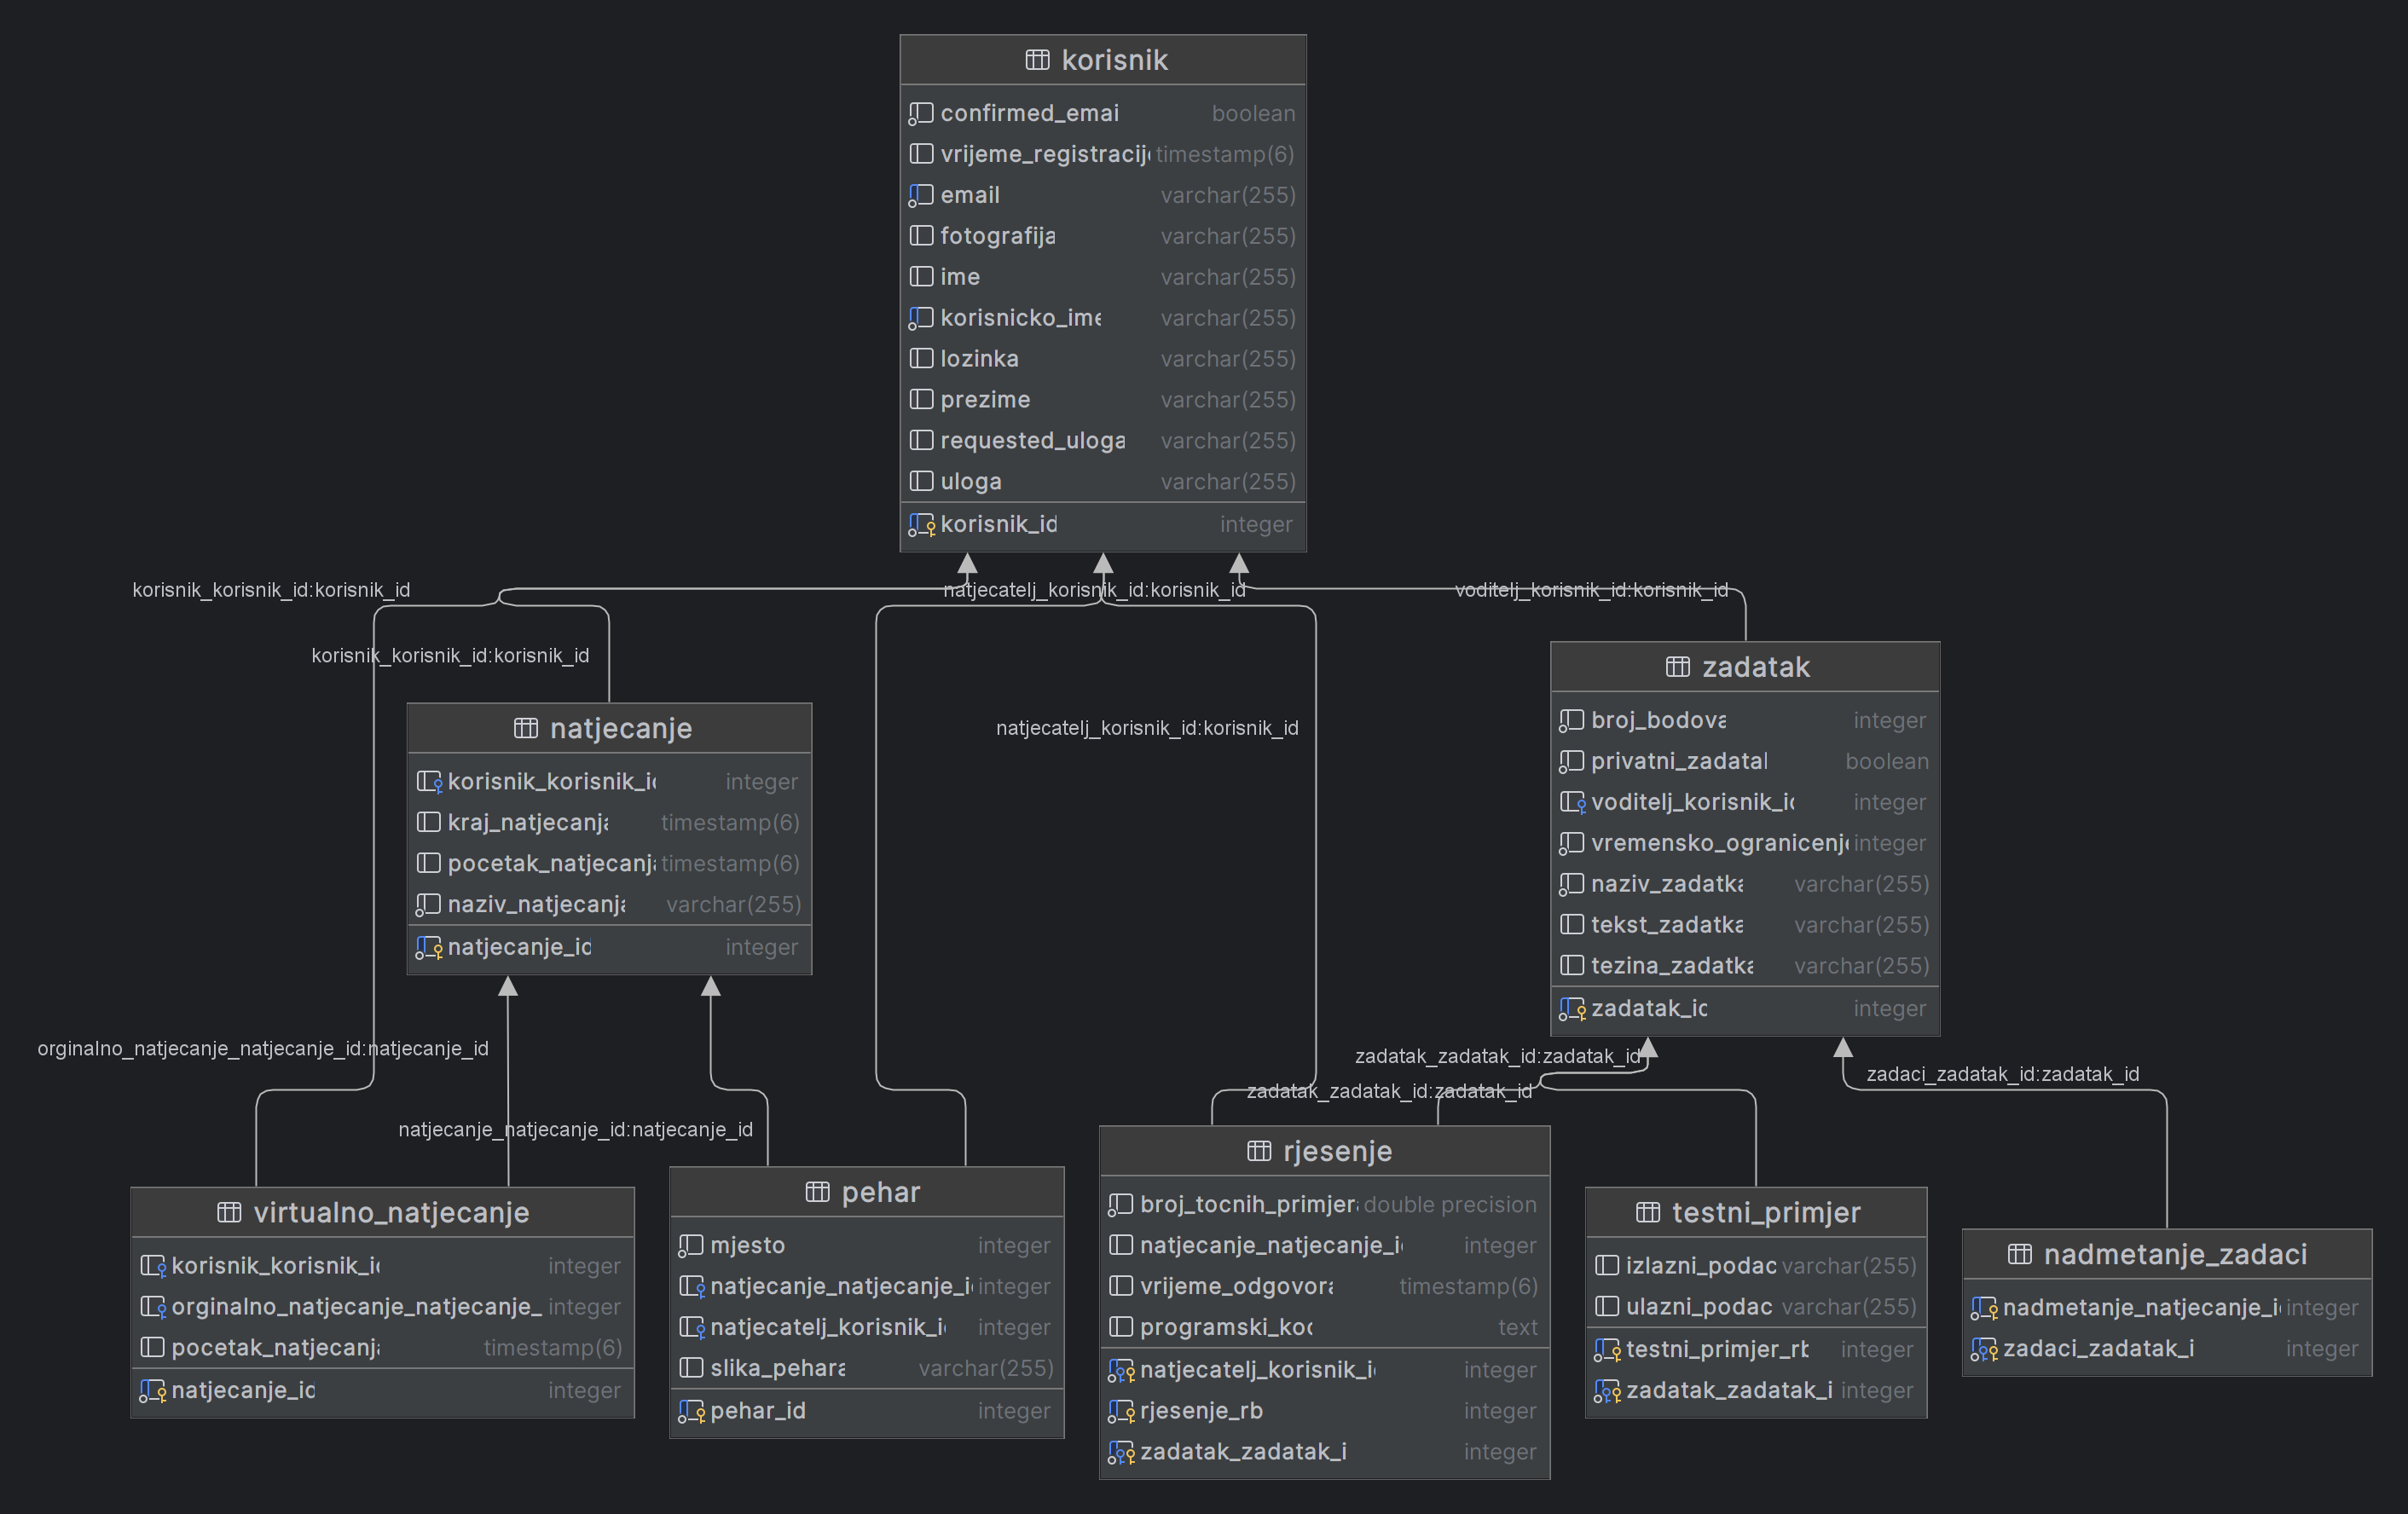
\includegraphics[scale=0.7]{dijagrami/dijagram_baze_podataka.png}
	\centering
	\caption{Dijagram baze podataka}
	\label{fig:bazaPodataka} 
\end{figure}

\eject


\section{Dijagram razreda}

Na slikama \ref{fig:dijagramRazreda1} i \ref{fig:dijagramRazreda2} prikazani su dijagrami razreda koji predstavljaju backend dio arhitekture.
Prva slika opisuje servise, odnosno njihovu implementaciju i prikazani su atributi i metode u pojedinim razredima.
Servisi predstavljaju glavnu logiku i oni su uglavnom u interakciji s repozitorijima koji su između ostalog prikazani na slici \ref{fig:dijagramRazreda2}.
Osim repozitorija, na slici \ref{fig:dijagramRazreda2} prikazani su i modeli (predstavljaju strukturu baze podataka) te kontroleri. 
Kontroleri su zaduženi za upravljanje HTTP zahtjevima i pružanje prikladnog odgovora. Na drugoj slici možemo uočiti atribute i međusobne odnose prethodno navedenih razreda. \\

Razred Korisnik predstavlja registriranog korisnika koji se može registrirati kao voditelj ili natjecatelj unoseći svoje podatke u sustav.
Razred Natjecanje definira naziv, početak i kraj natjecanja te voditelja. Razred Pehar je entitet u kojeg spremamo koje mjesto je osvojio natjecatelj na nekom natjecanju i sliku pehara.
Razred uloga je enumeracija koja definira ulogu korisnika (admin, natjecatelj ili voditelj). Razred zadatak je entitet koji predstavlja određeni problem na natjecanju i sadrži referencu na testne primjere.
Testni primjer sadrži informacije o tesnim primjerima za pojedinačni zadatak. Razred Rjesenje predstavlja predano rješenje pojedinog korisnika za zadatak. 
Razred Virtualno natjecanje predstavlja natjecanje koje se može naknadno pokrenuti i rješavati. 

\begin{figure}[H]
	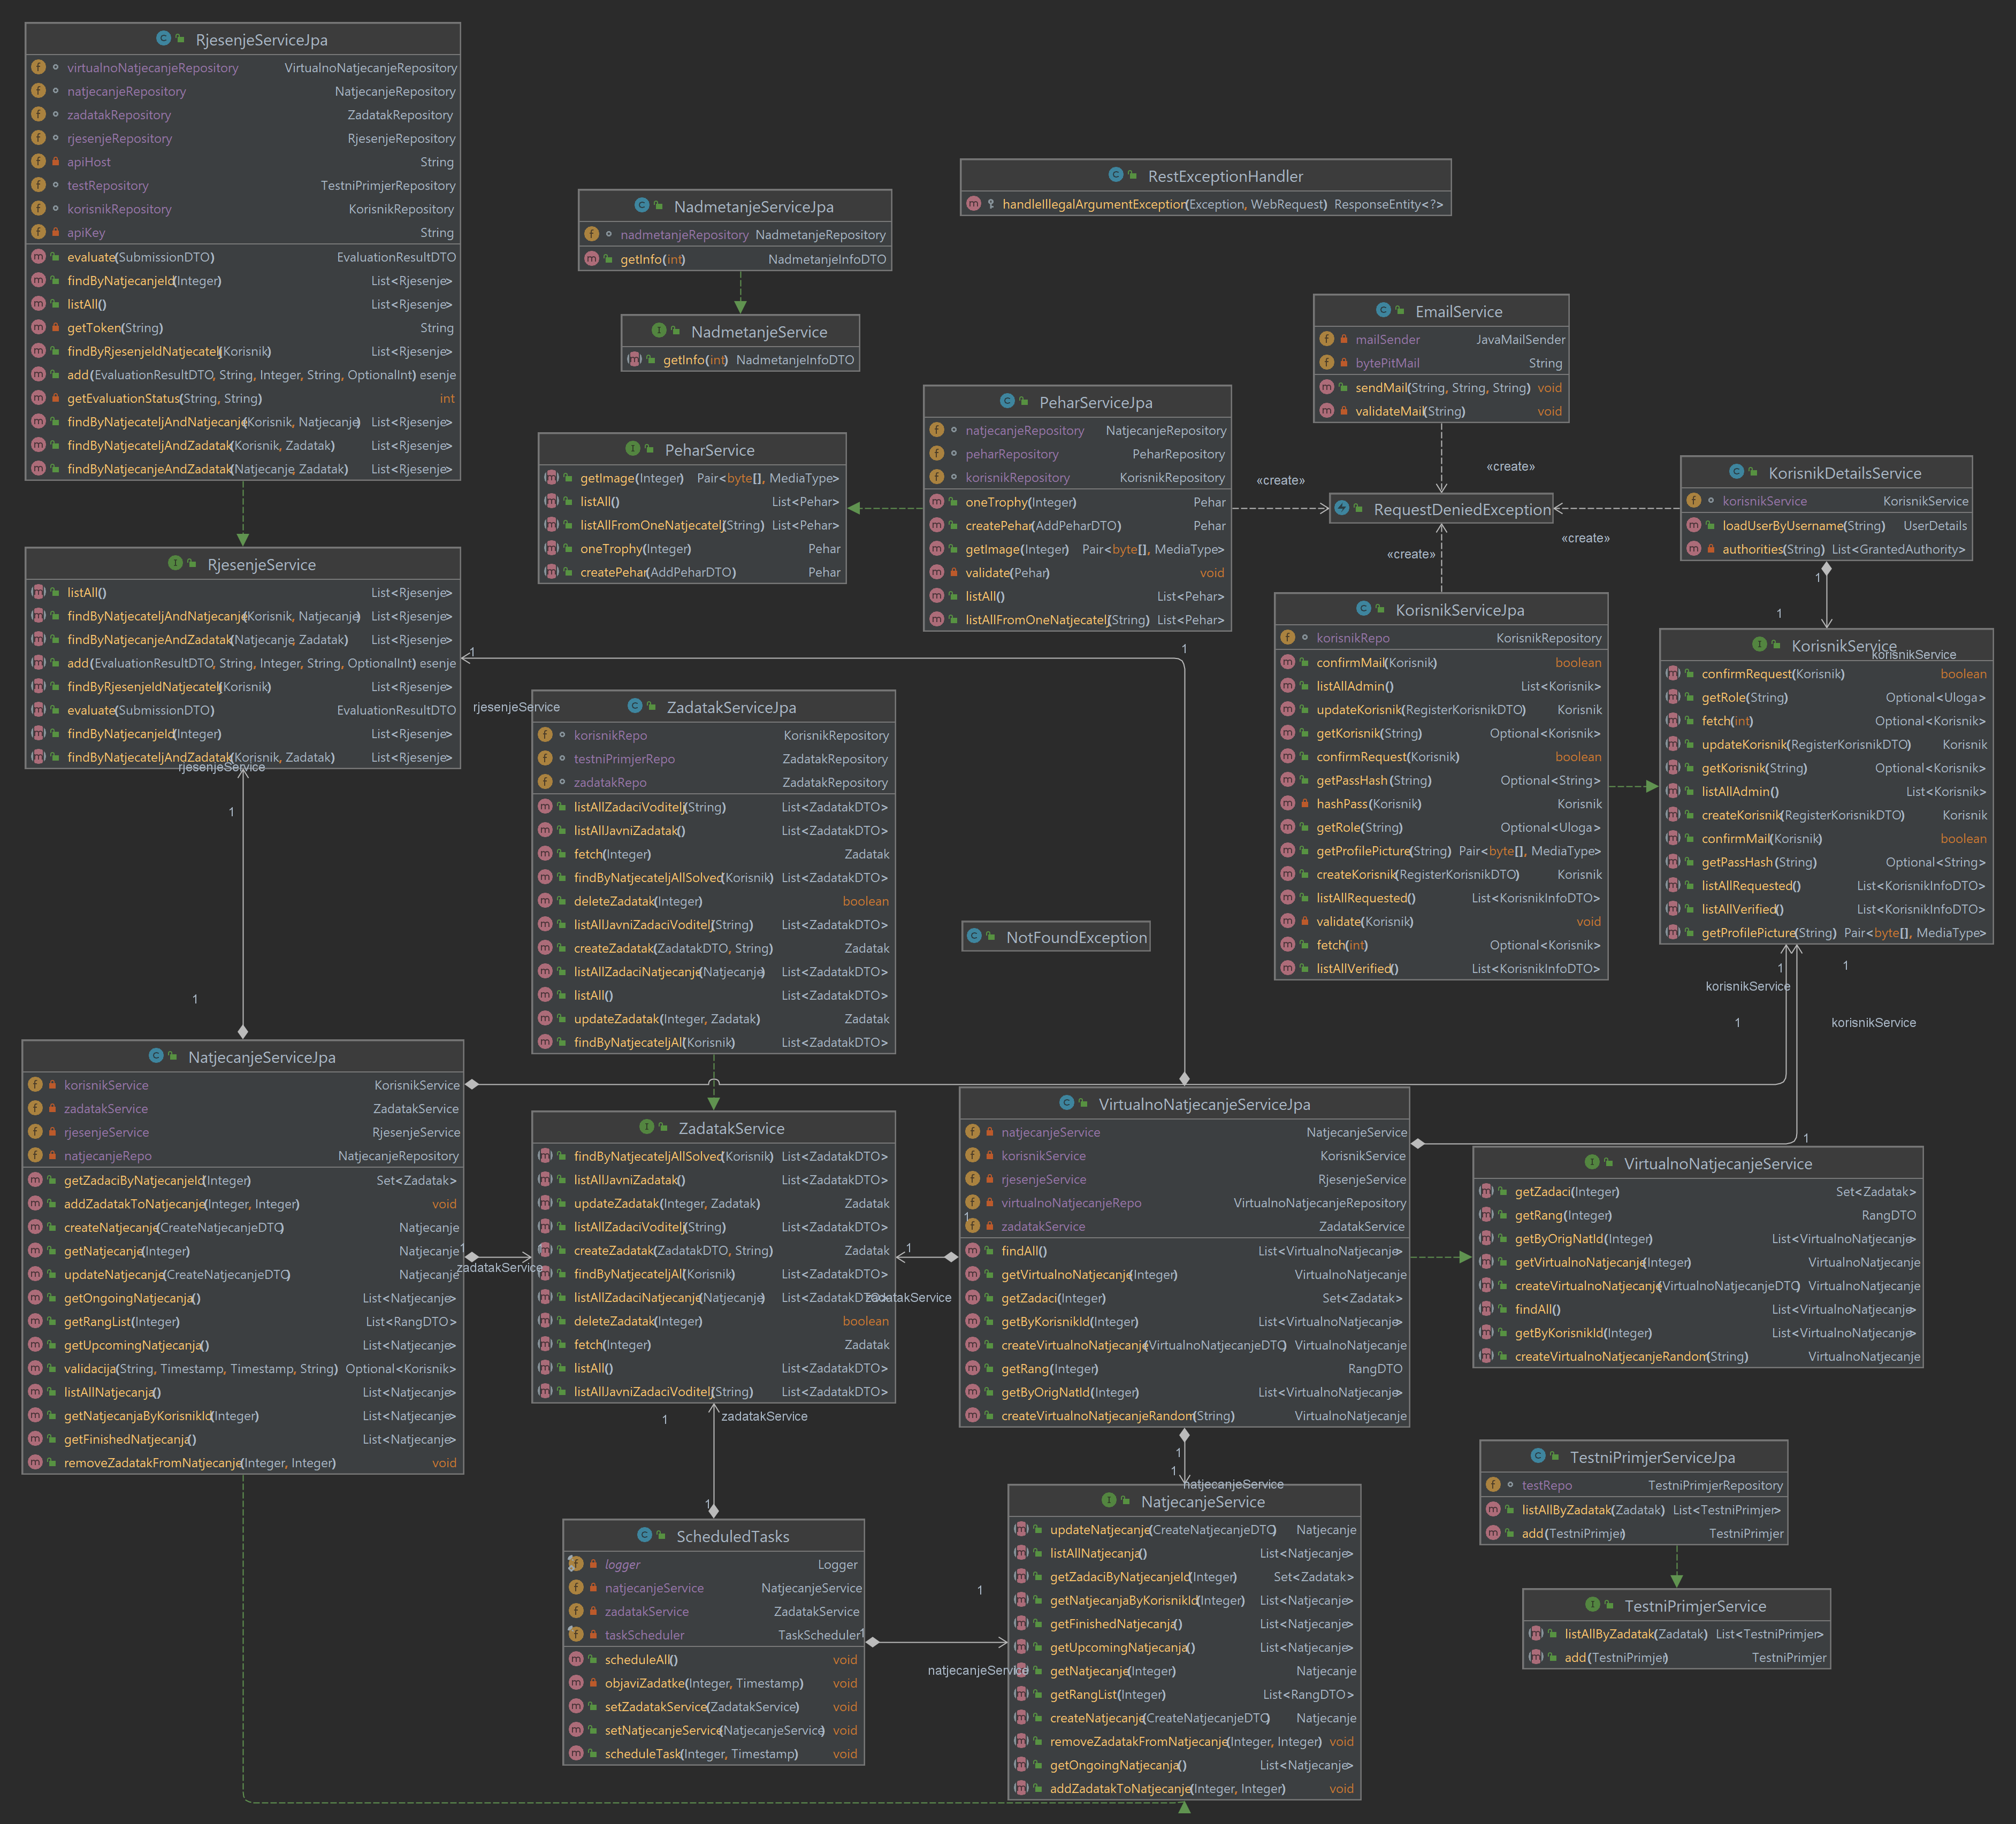
\includegraphics[scale=0.19]{dijagrami/serviceDiagram.png}
	\centering
	\caption{Dijagram razreda - Servisi}
	\label{fig:dijagramRazreda1}
\end{figure}

\begin{figure}[H]
	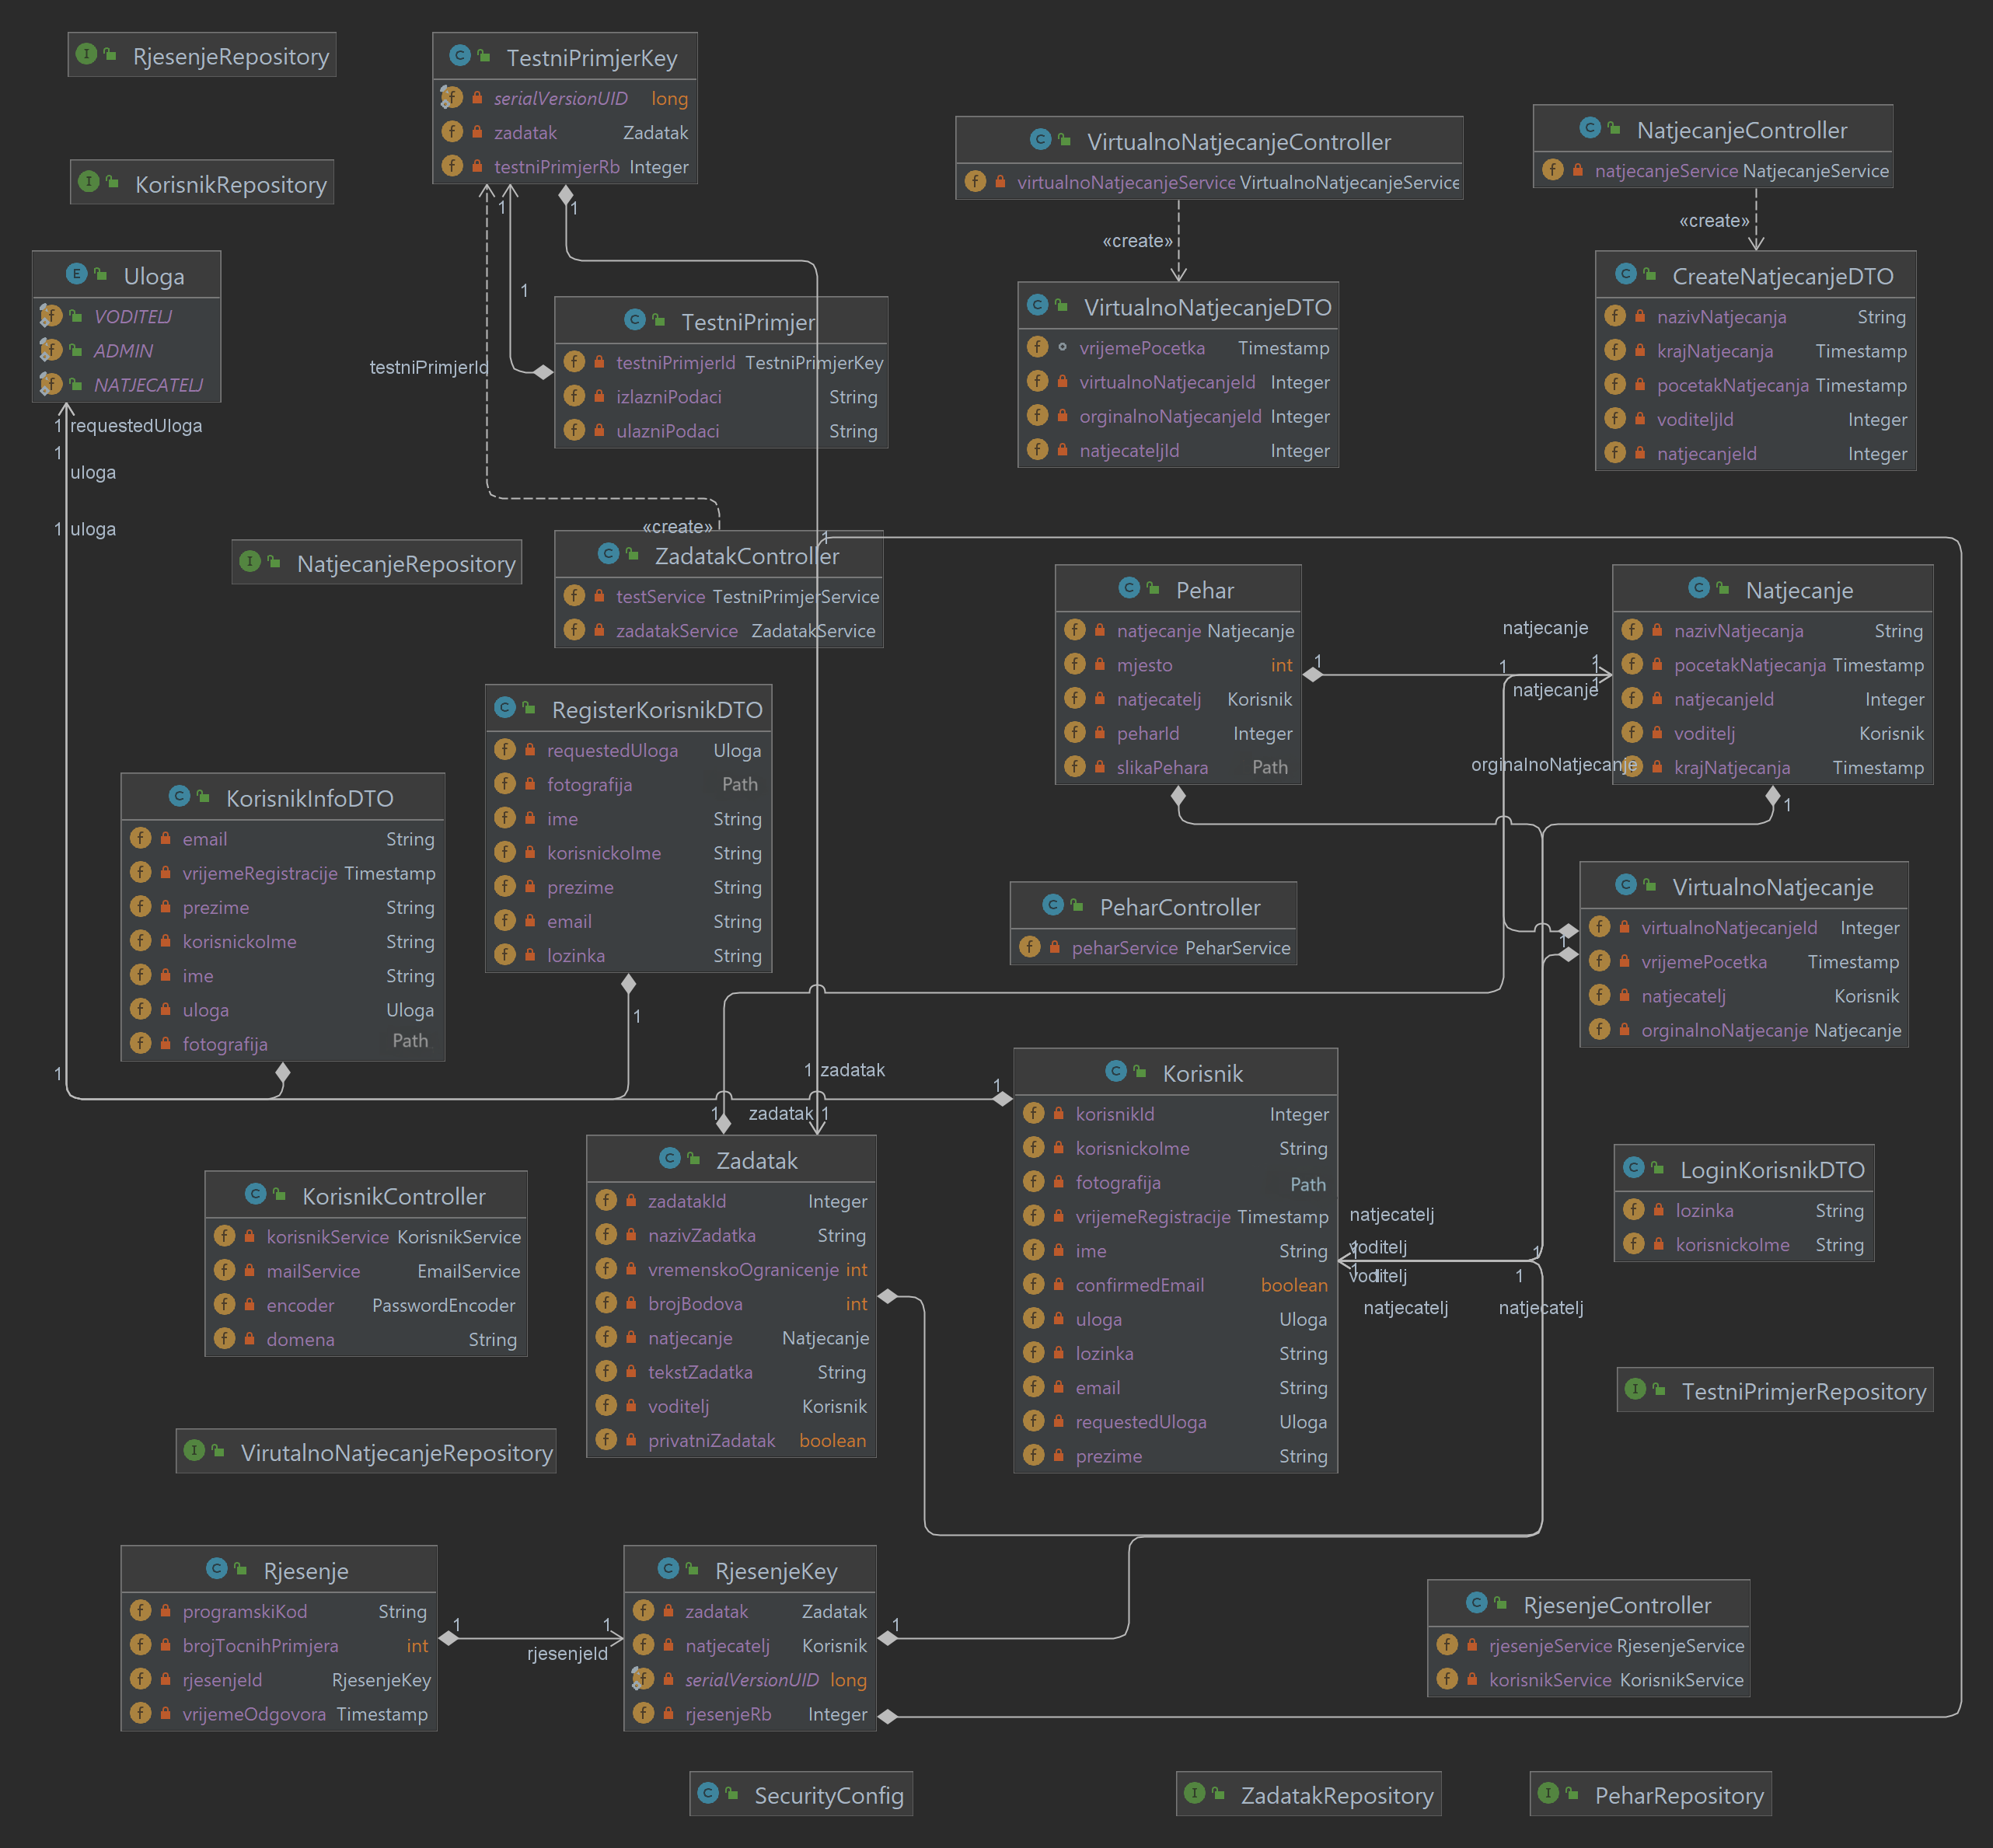
\includegraphics[scale=0.2]{dijagrami/apiDiagram.png}
	\centering
	\caption{Dijagram razreda - Kontroleri, Repozitoriji i Modeli}
	\label{fig:dijagramRazreda2}
\end{figure}

%\textbf{\textit{dio 2. revizije}}\\
%
%\textit{Prilikom druge predaje projekta dijagram razreda i opisi moraju odgovarati stvarnom stanju implementacije}
%
%
%
%\eject
%
%\section{Dijagram stanja}
%
%
%\textbf{\textit{dio 2. revizije}}\\
%
%\textit{Potrebno je priložiti dijagram stanja i opisati ga. Dovoljan je jedan dijagram stanja koji prikazuje \textbf{značajan dio funkcionalnosti} sustava. Na primjer, stanja korisničkog sučelja i tijek korištenja neke ključne funkcionalnosti jesu značajan dio sustava, a registracija i prijava nisu. }
%
%
%\eject
%
\section{Dijagram aktivnosti}

Dijagram aktivnosti na slici \ref{fig:dijagramAktivnosti} prikazuje proces kreiranja novog natjecanja. Voditelj se prijavljuje u sustav te nakon uspješne prijave odabire opciju za organiziranje novog natjecanja. Web stranica preko baze podataka dohvaća dostupne zadatke te ih prikazuje kao dio forme u koju voditelj unosi podatke te odabire zadatke koji će se ispitivati u sklopu natjecanja. Nakon slanja unesenih podataka web aplikaciji, ona ih prosljeđuje bazi podataka koja ih zatim pohranjuje i šalje potvrdu o uspješnom stvaranju novog natjecanja. 
\\
\begin{figure}[H]
	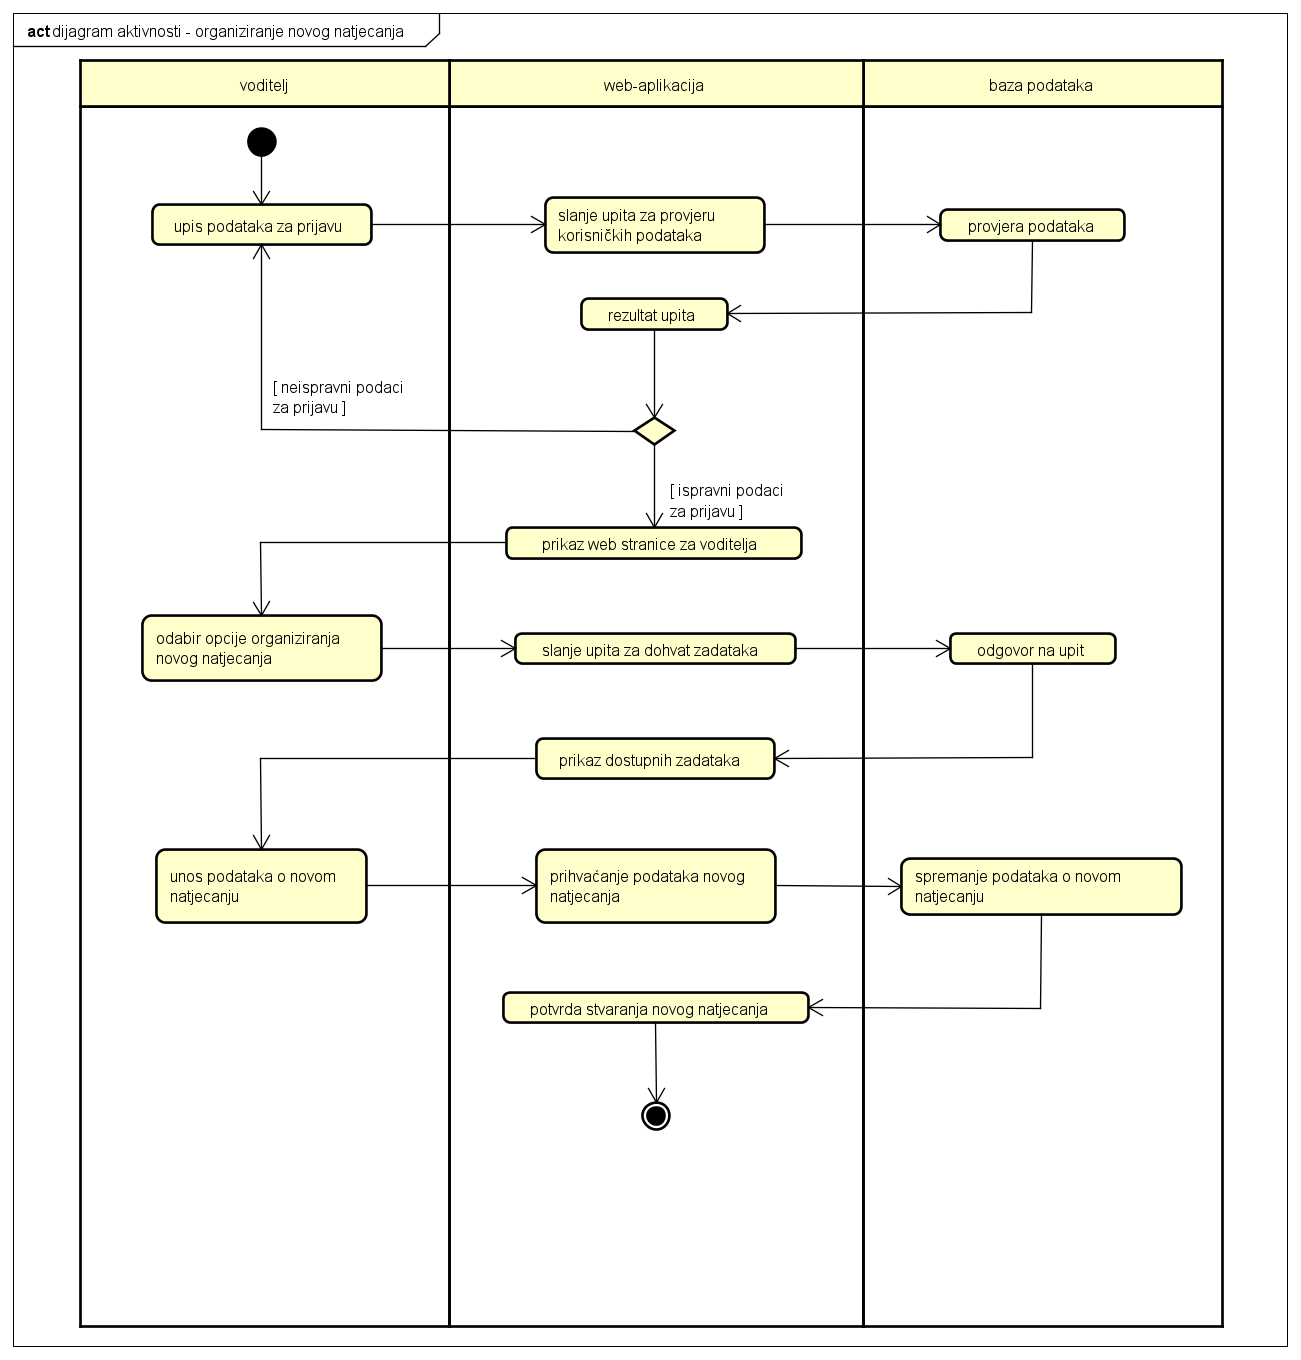
\includegraphics[scale=0.5]{dijagrami/act_novo_natjecanje.png}
	\centering
	\caption{Dijagram aktivnosti - organiziranje novog natjecanja}
	\label{fig:dijagramAktivnosti}
\end{figure}
%
%\textbf{\textit{dio 2. revizije}}\\
%
%\textit{Potrebno je priložiti dijagram aktivnosti s pripadajućim opisom. Dijagram aktivnosti treba prikazivati značajan dio sustava.}
%
%\eject
\section{Dijagram komponenti}

Dijagram komponenti prikazan na slici \ref{fig:dijagramKomponenti} opisuje organizaciju i međuovisnost  komponenti, interne strukture i odnose prema okolini. Web aplikacija sastoji se od komponenti: Controllers, Services, Repositories, DTO i Models. Controllers pruža REST API sučelje na koje vanjski web preglednik može slati zahtjeve i primati odgovore pomoću JSON datoteka. Repositories pristupa SQL bazi podataka koja ostvaruje sučelje SQL API. Podaci koji su pristigli iz baze se šalju dalje MVC arhitekturi u obliku DTO(Data transfer objcet). Repositories upisuje podatke iz baze podataka u komponentu Services. Models oblikuje korištene entitete i njihov međuodnos. Controllers šalje i prima podatke od komponente Services. Controllers pruža MAIL API sučelje Mailjet preko kojeg šalje mailove i Judge0 API za evaluaciju programskog rješenja.
\\
\begin{figure}[H]
	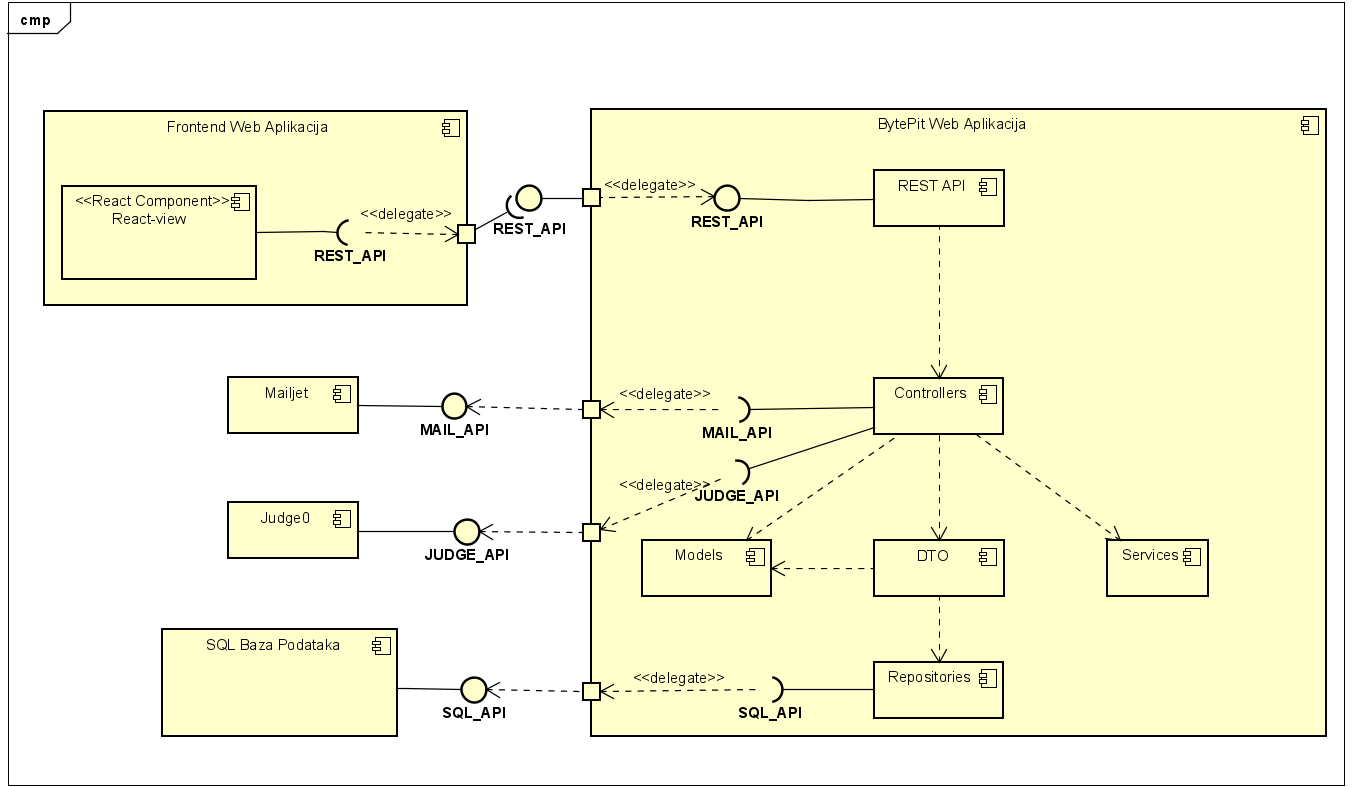
\includegraphics[scale=0.5]{dijagrami/dijagramKomponenti.png}
	\centering
	\caption{Dijagram komponenti}
	\label{fig:dijagramKomponenti}
\end{figure}
%
%\textbf{\textit{dio 2. revizije}}\\
%
%\textit{Potrebno je priložiti dijagram komponenti s pripadajućim opisom. Dijagram komponenti treba prikazivati strukturu cijele aplikacije.}

	\chapter{Implementacija i korisničko sučelje}


\section{Korištene tehnologije i alati}

\noindent Za komunikaciju tima korištene su aplikacije \underline{WhatsApp}\footnote{https://www.whatsapp.com/} i \underline{Discord}\footnote{https://discord.com}. Za izradu UML dijagrama korišten je \underline{Astah Professional}\footnote{http://astah.net/editions/professional}.

Za izradu dokumentacije korišten je \underline{LaTeX}\footnote{https://www.latex-project.org}, sustav za izradu dokumenata koji koristi markup jezik. Za upravljanje izvornim kodom korišten je \underline{Git}\footnote{https://git-scm.com/}. Repozitorij projekta dostupan je na platformi \underline{GitHub}\footnote{https://github.com}.

Za razvojna okruženja korišteni su \underline{Visual Studio Code}\footnote{https://visualstudio.microsoft.com/}. Visual Studio Code je integrirano razvojno okruženje (IDE) kompanije Microsoft. Koristi se za razvoj wen-stranica, web-aplikacija, web-usluga i mobilnih aplikacija. Za razvoj softvera koristi Windows API, Windows Forms, Windows Presentation Foundation, Windows Store i Microsoft Silverlight.

Za pisanje aplikacije korišten je \underline{Spring Boot}\footnote{https://spring.io/projects/spring-boot/}, framework za razvoj Java aplikacija, za razvoj backenda. Za razvoj frontenda korišten je \underline{React}\footnote{https://react.dev}, biblioteka za izgradnju sučelja u jeziku \underline{JavaScript}\footnote{https://www.javascript.com/}. Također je korišten \underline{TypeScript}\footnote{https://www.typescriptlang.org} kao nadrogradnja nad JavaScriptom. On poboljšava kvalitetu i održivost koda napisanog u JavaScriptu.

Baza podataka nalazi se na poslužitelju 

\eject


\section{Ispitivanje programskog rješenja}

%\textbf{\textit{dio 2. revizije}}\\

%\textit{U ovom poglavlju je potrebno opisati provedbu ispitivanja implementiranih funkcionalnosti na razini komponenti i na razini cijelog sustava s prikazom odabranih ispitnih slučajeva. Studenti trebaju ispitati temeljnu funkcionalnost i rubne uvjete.}


\subsection{Ispitivanje komponenti}
U procesu testiranja funkcionalnosti komponenti,  koristili smo popularni radni okvir \textit{JUnit}. Kako bi testiranje bilo izolirano, potrebno je simulirati komponente o kojima ovisi komponenta koju testiramo. U tu svrhu smo koristili programski okvir \textit{Mockito}. Ukupno smo implementirali sedam testirajućih metoda unutar tri testirajuće klase.

\vspace{1em}

U svrhu testiranja funkcionalnosti klase \textit{KorisnikController}, implementirali smo tri metode. Specifično, testirajuća metoda \ref{fig:test1} ima za cilj provjeriti ispravnost metode za registraciju novog korisnika kada su joj proslijeđeni valjani podaci za registraciju (ime, prezime, korisničko ime, lozinka, e-mail i uloga) te slika profila. Očekujemo da će rezultat testirane metode biti objekt tipa \textit{Korisnik}, koji će sadržavati točne podatke (prethodno proslijeđene) o novostvorenom korisniku.

\begin{figure}[H]
	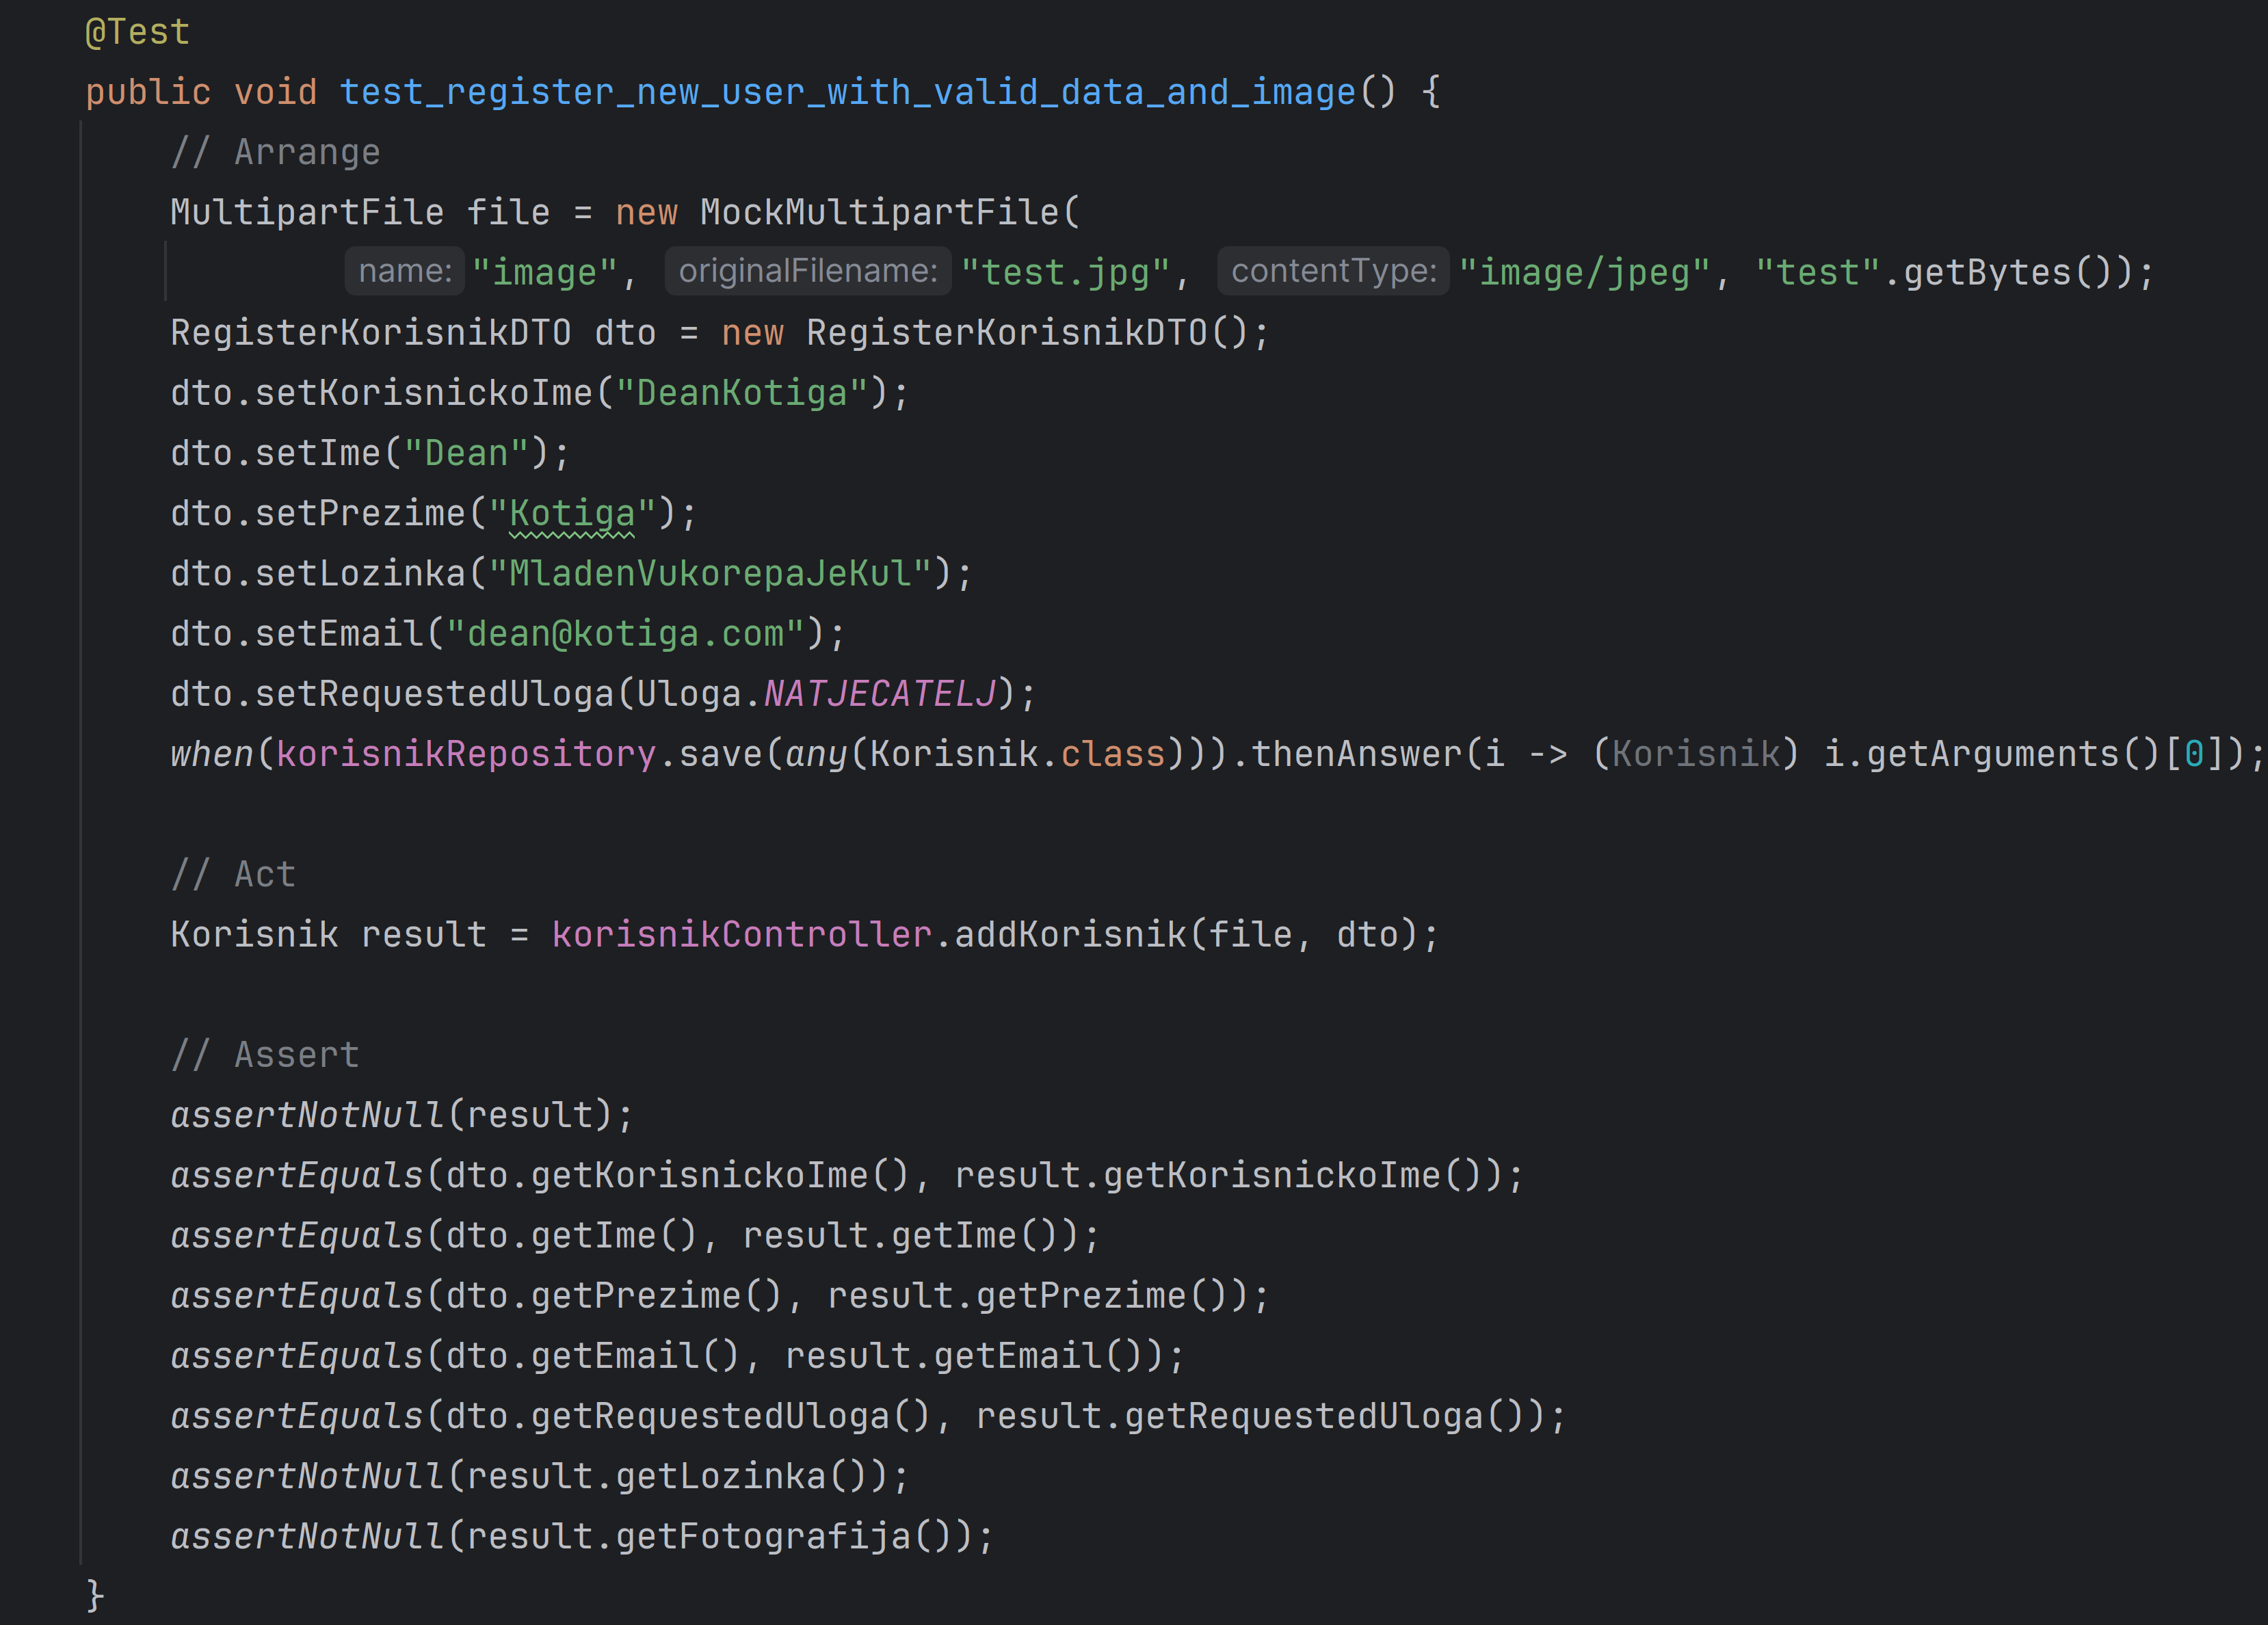
\includegraphics[scale=0.15]{slike/test1.png}
	\centering
	\caption{Testirajuća metoda - registracija korisnika}
	\label{fig:test1}
\end{figure}

Za razliku od prethodne, testirajuća metoda \ref{fig:test2} provjerava ispravnost iste metode u situaciji kada se pokuša dodati korisnik s korisničkim imenom koje je već zauzeto.  U ovome ispitnom slučaju se očekuje da će testirana metoda prepoznati ovu situaciju i shodno tome baciti očekivanu iznimku.

\begin{figure}[H]
	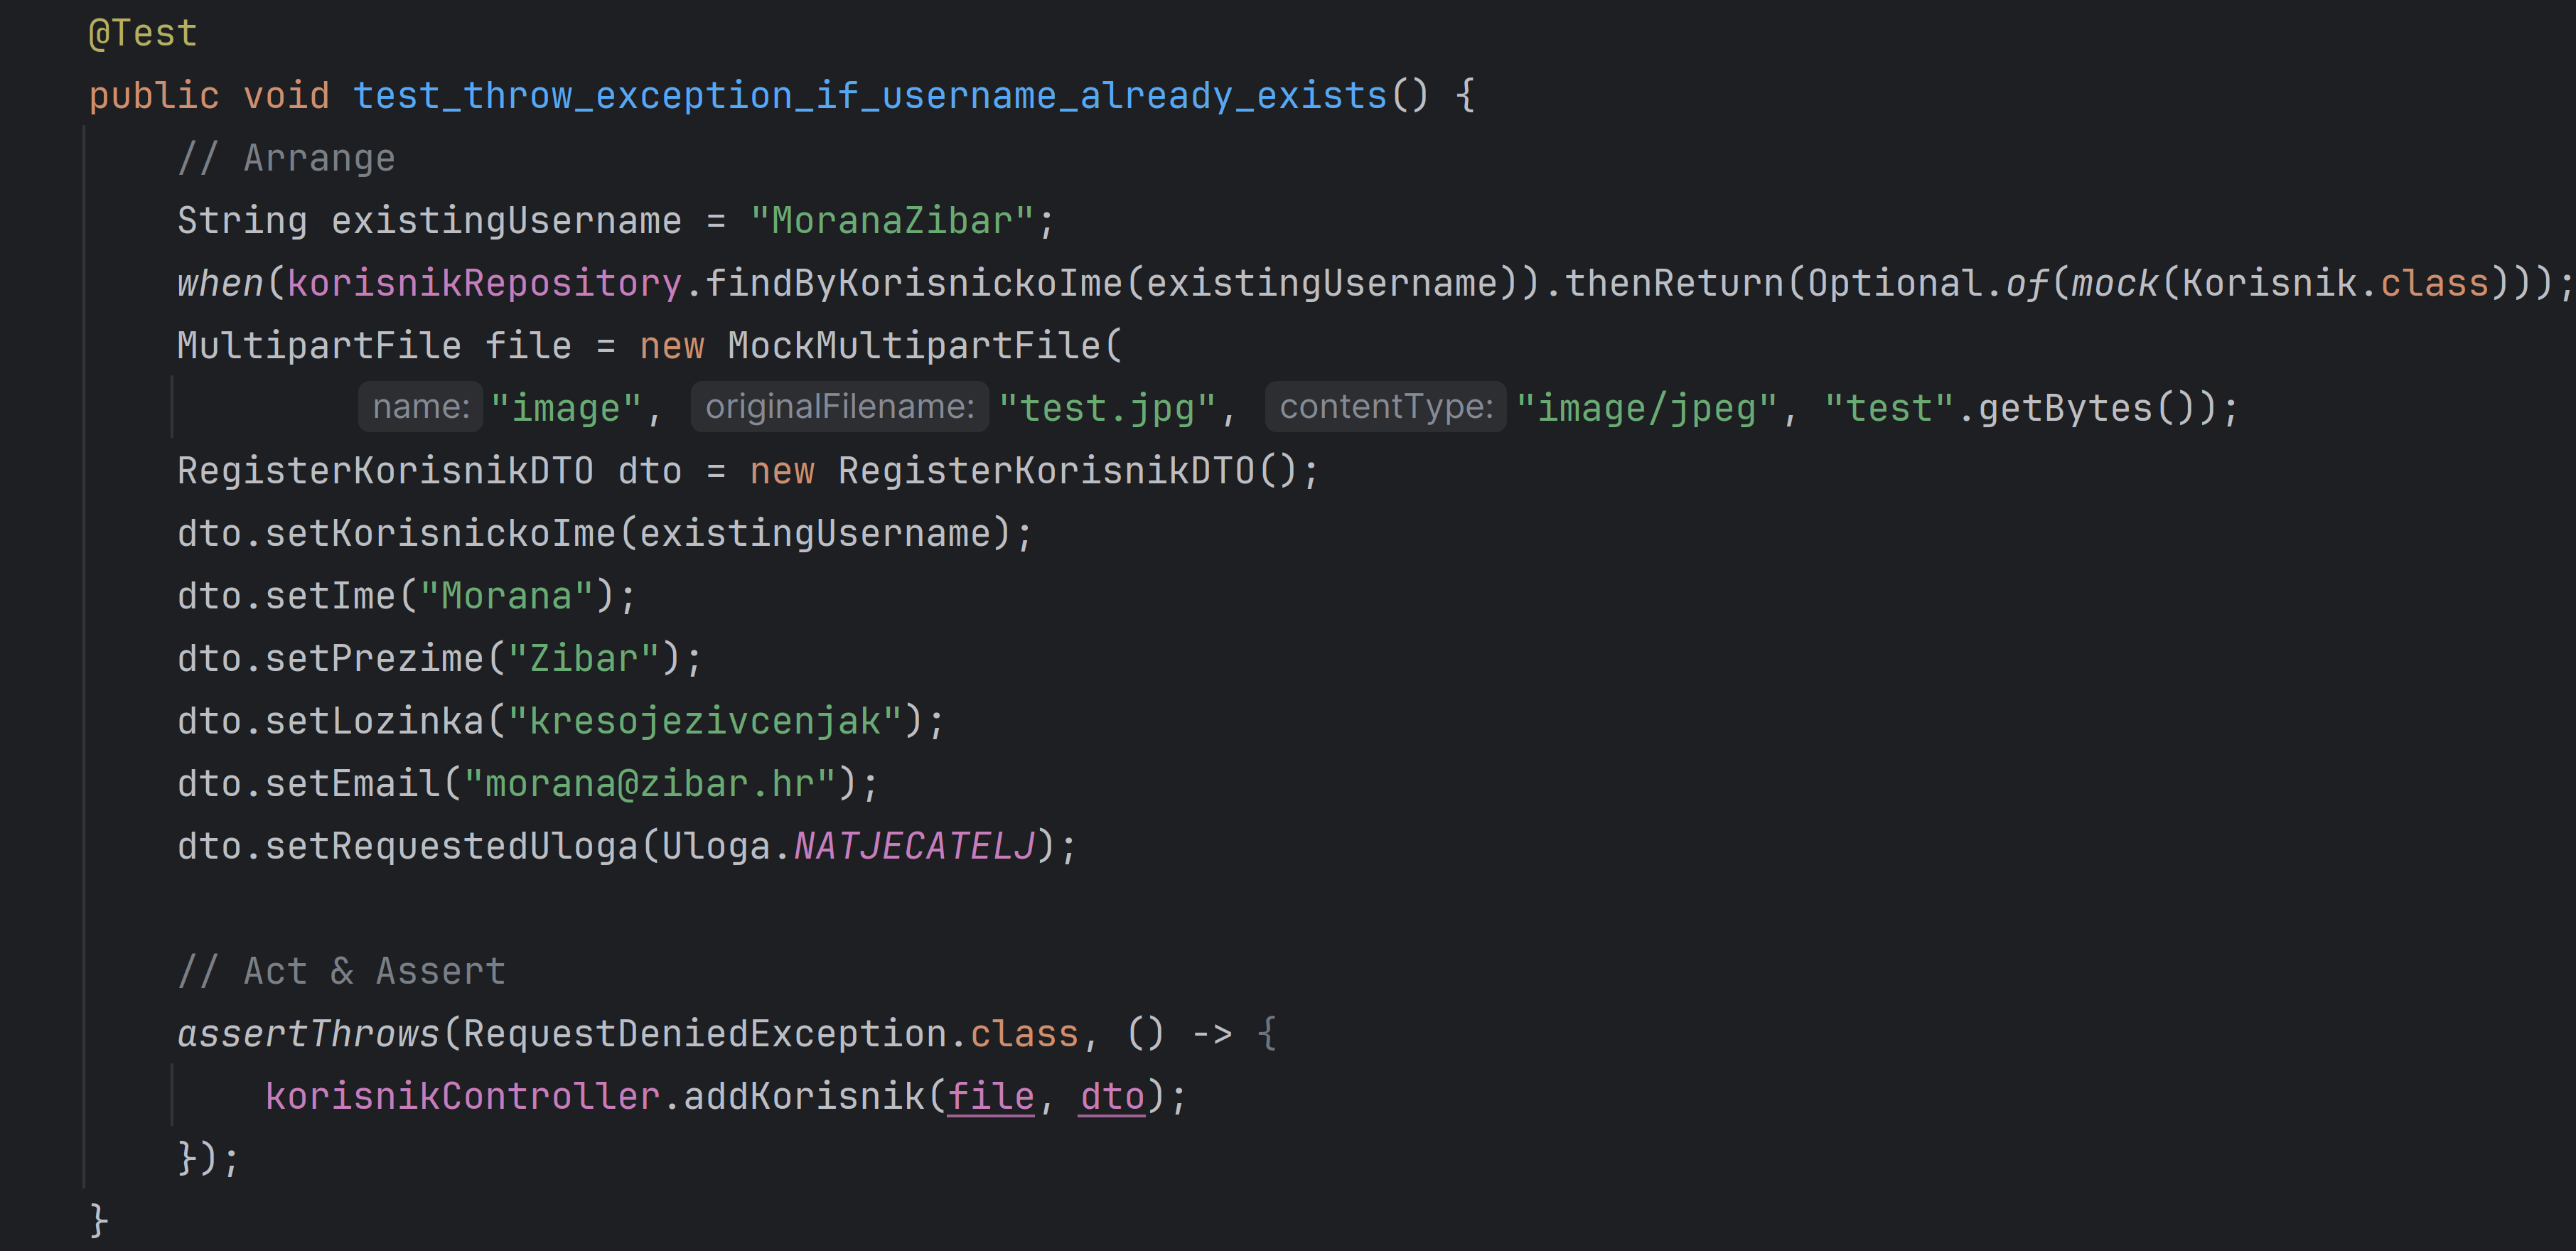
\includegraphics[scale=0.15]{slike/test2.png}
	\centering
	\caption{Testirajuća metoda - neuspješna registracija korisnika}
	\label{fig:test2}
\end{figure}

Posljednjim ispitnim slučajem \ref{fig:test3} za klasu \textit{KorisnikController} želimo verificirati  ispravnost metode za potvrdu zahtijevanih uloga korisnika od strane administratora. Očekuje se da će nakon uspješne potvrde testirana metoda, koja kao argument prima korisničko ime, vratiti HTTP odgovor sa statusom OK.

\begin{figure}[H]
	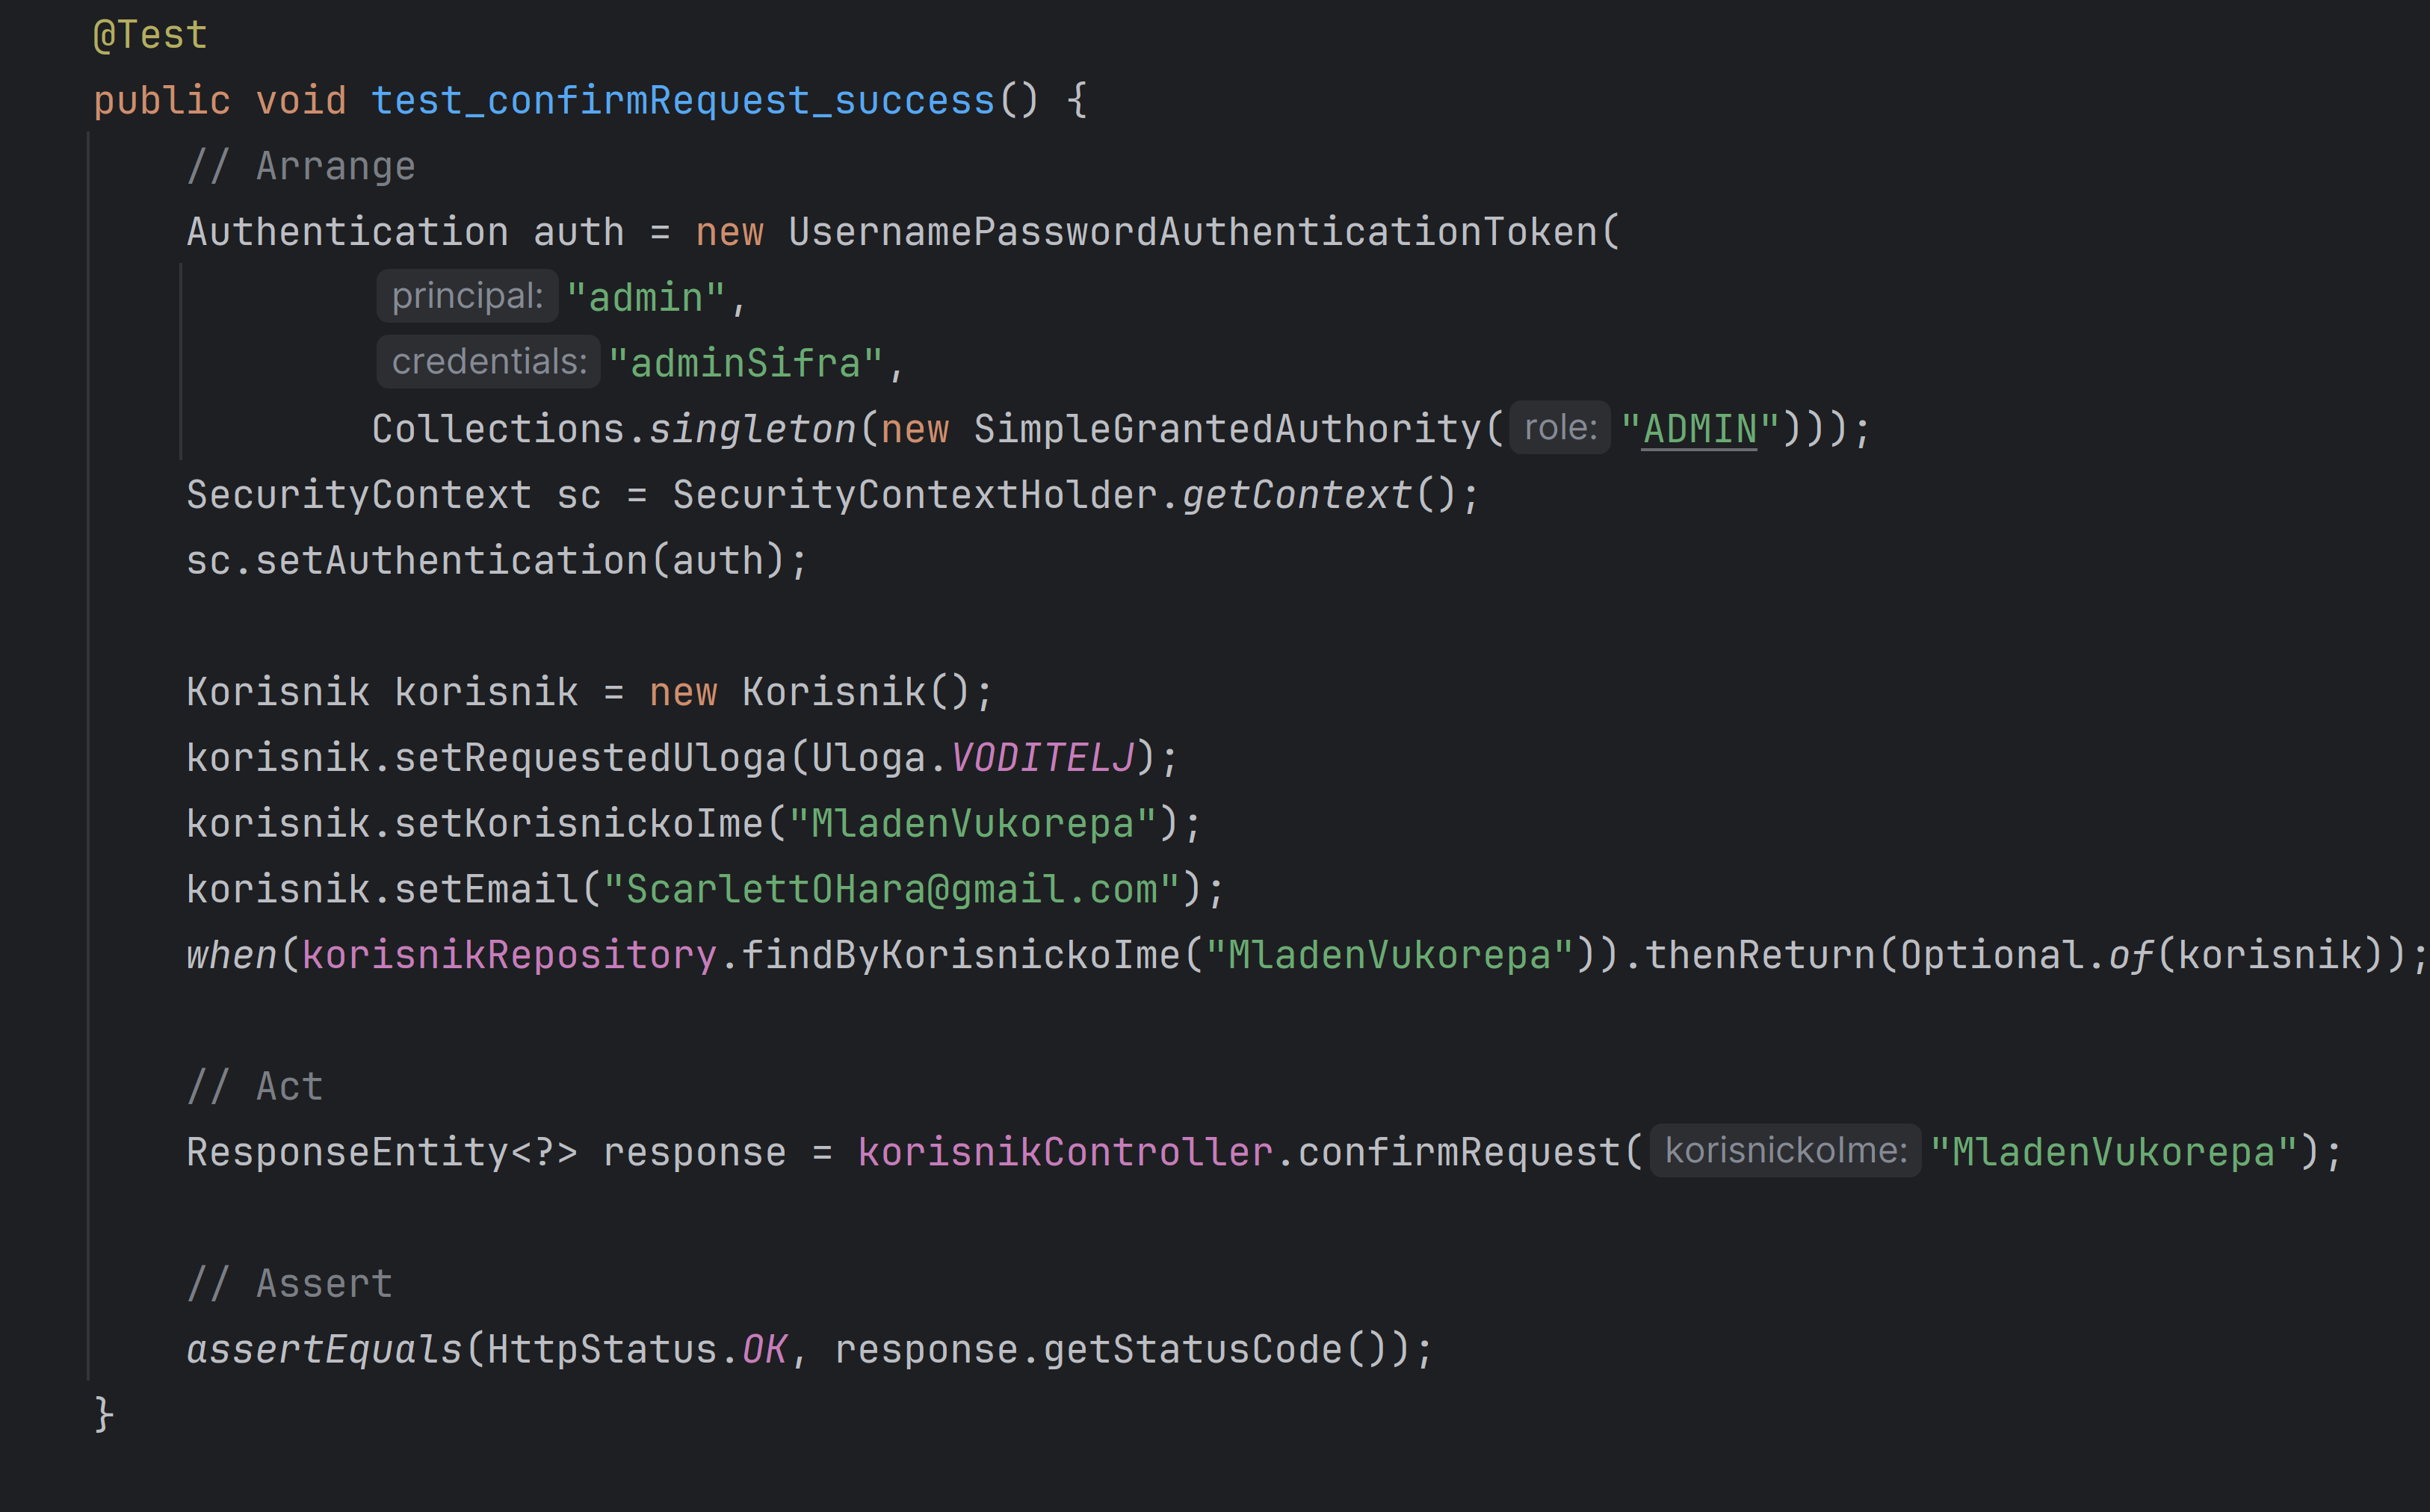
\includegraphics[scale=0.15]{slike/test3.png}
	\centering
	\caption{Testirajuća metoda - potvrda zatražene uloge}
	\label{fig:test3}
\end{figure}

S ciljem testiranja klase \textit{NatjecanjeController} napisana su dva testa. Testirajućom metodom 5.4 želimo provjeriti ispravnost metode za stvaranje novog natjecanja kada su pruženi ispravni ulazni podaci (naziv, voditelj, početak i kraj natjecanja). Očekuje se da će nakon uspješnog stvaranja natjecanja, testirana metoda vratiti odgovarajući objekt \textit{CreateNatjecanjeDTO} koji sadrži proslijeđene ulazne podatke o novostvorenom natjecanju.

\begin{figure}[H]
	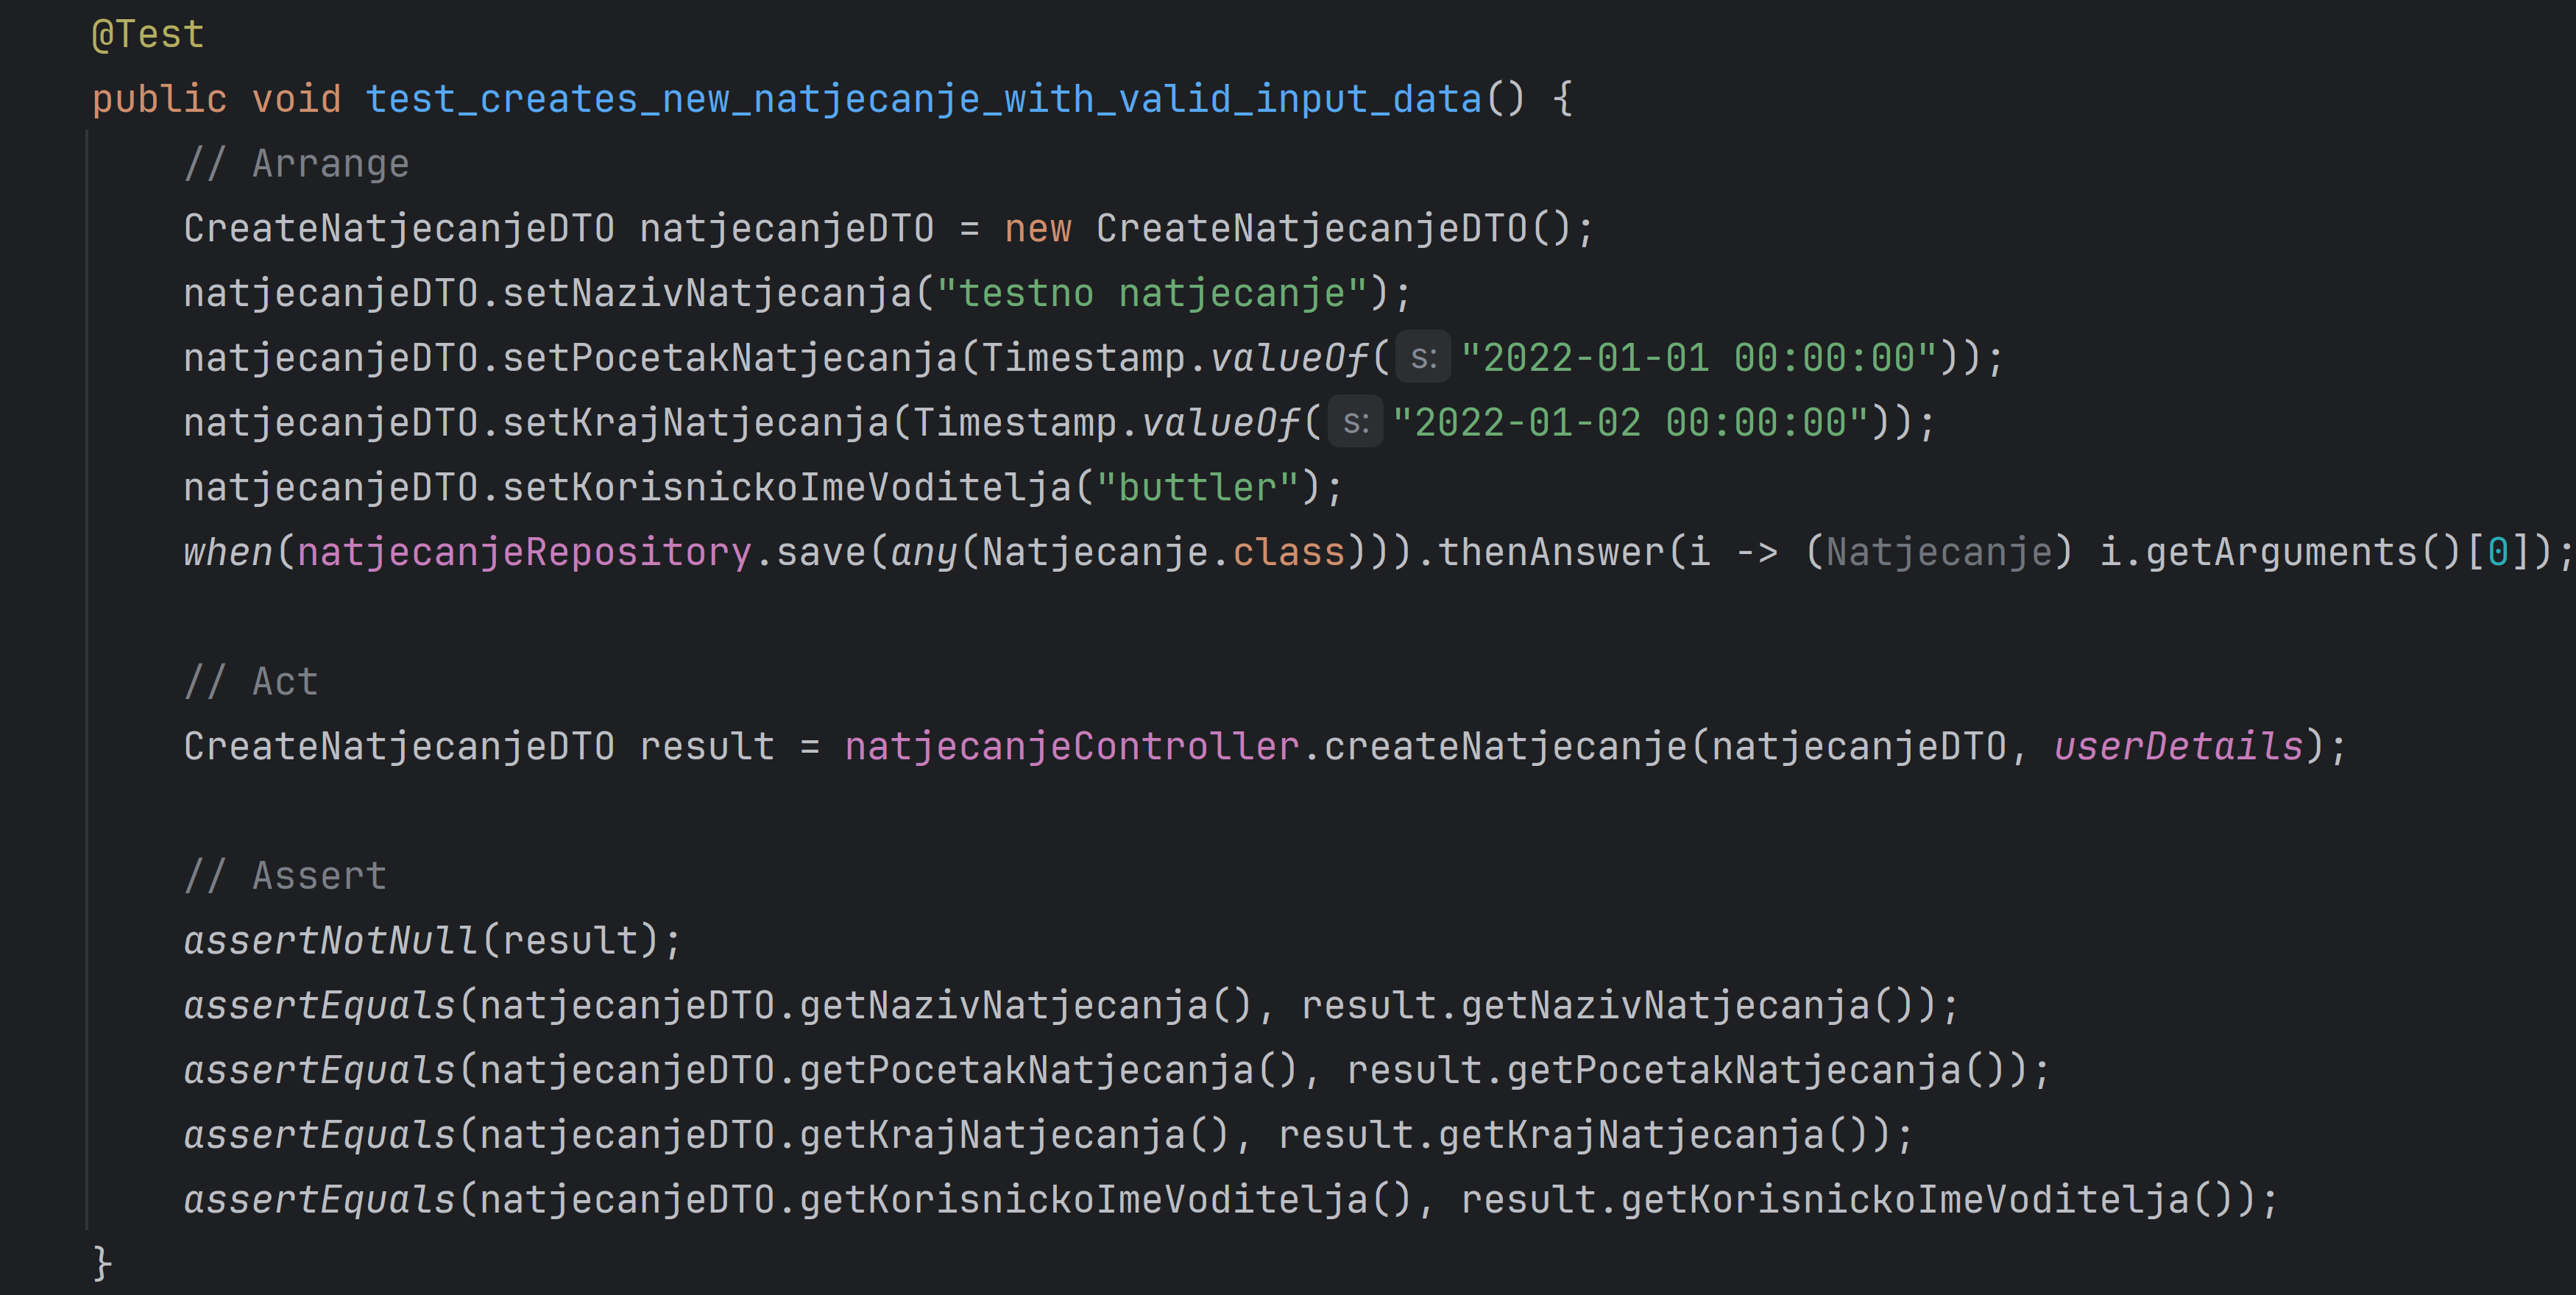
\includegraphics[scale=0.15]{slike/test4.png}
	\centering
	\caption{Testirajuća metoda - stvaranje natjecanja}
	\label{fig:test4}
\end{figure}

Druga i posljednja testirajuća metoda \ref{fig:test5} za klasu \textit{NatjecanjeController} ima za cilj provjeriti ispravnost iste metode u situaciji kada je odabrani početak natjecanja nakon završetka natjecanja. Očekuje se da će u takvim slučajevima metoda baciti iznimku.

\begin{figure}[H]
	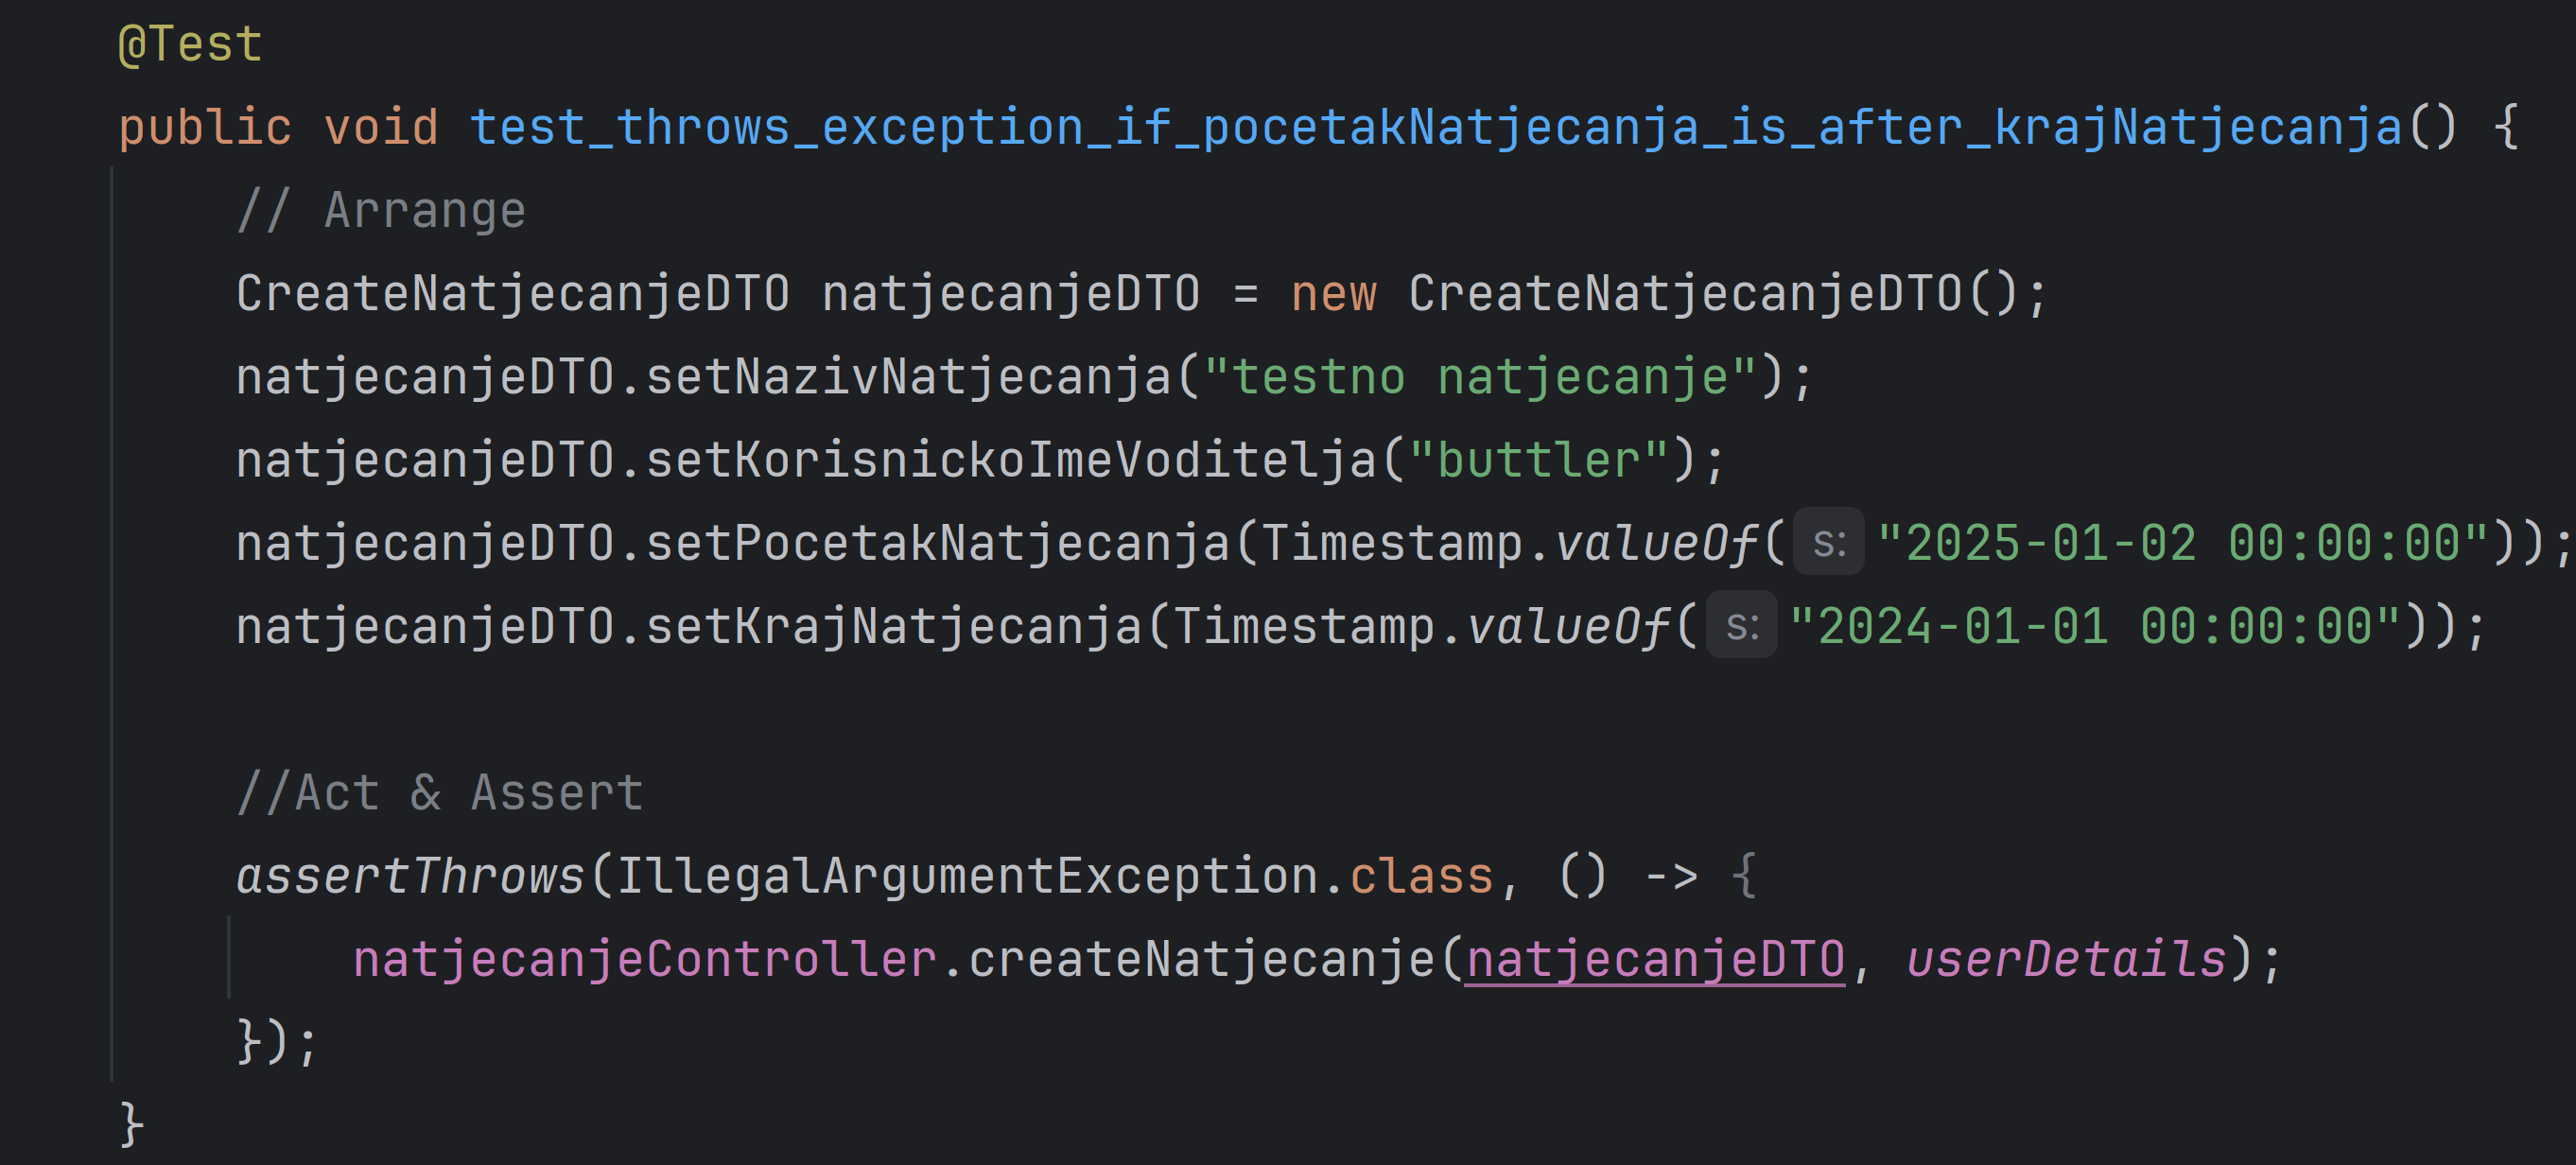
\includegraphics[scale=0.2]{slike/test5.png}
	\centering
	\caption{Testirajuća metoda - neuspješno stvaranje natjecanja}
	\label{fig:test5}
\end{figure}

Na kraju, implementirana su i dva testa za klasu \textit{ZadatakController}. U metodi \ref{fig:test6}, fokusirali smo se na testiranje metode koja dohvaća sve javne zadatke, s posebnim naglaskom na rubni slučaj kada nema dostupnih javnih zadataka. U toj situaciji očekujemo praznu listu kao povratnu vrijednost.

\begin{figure}[H]
	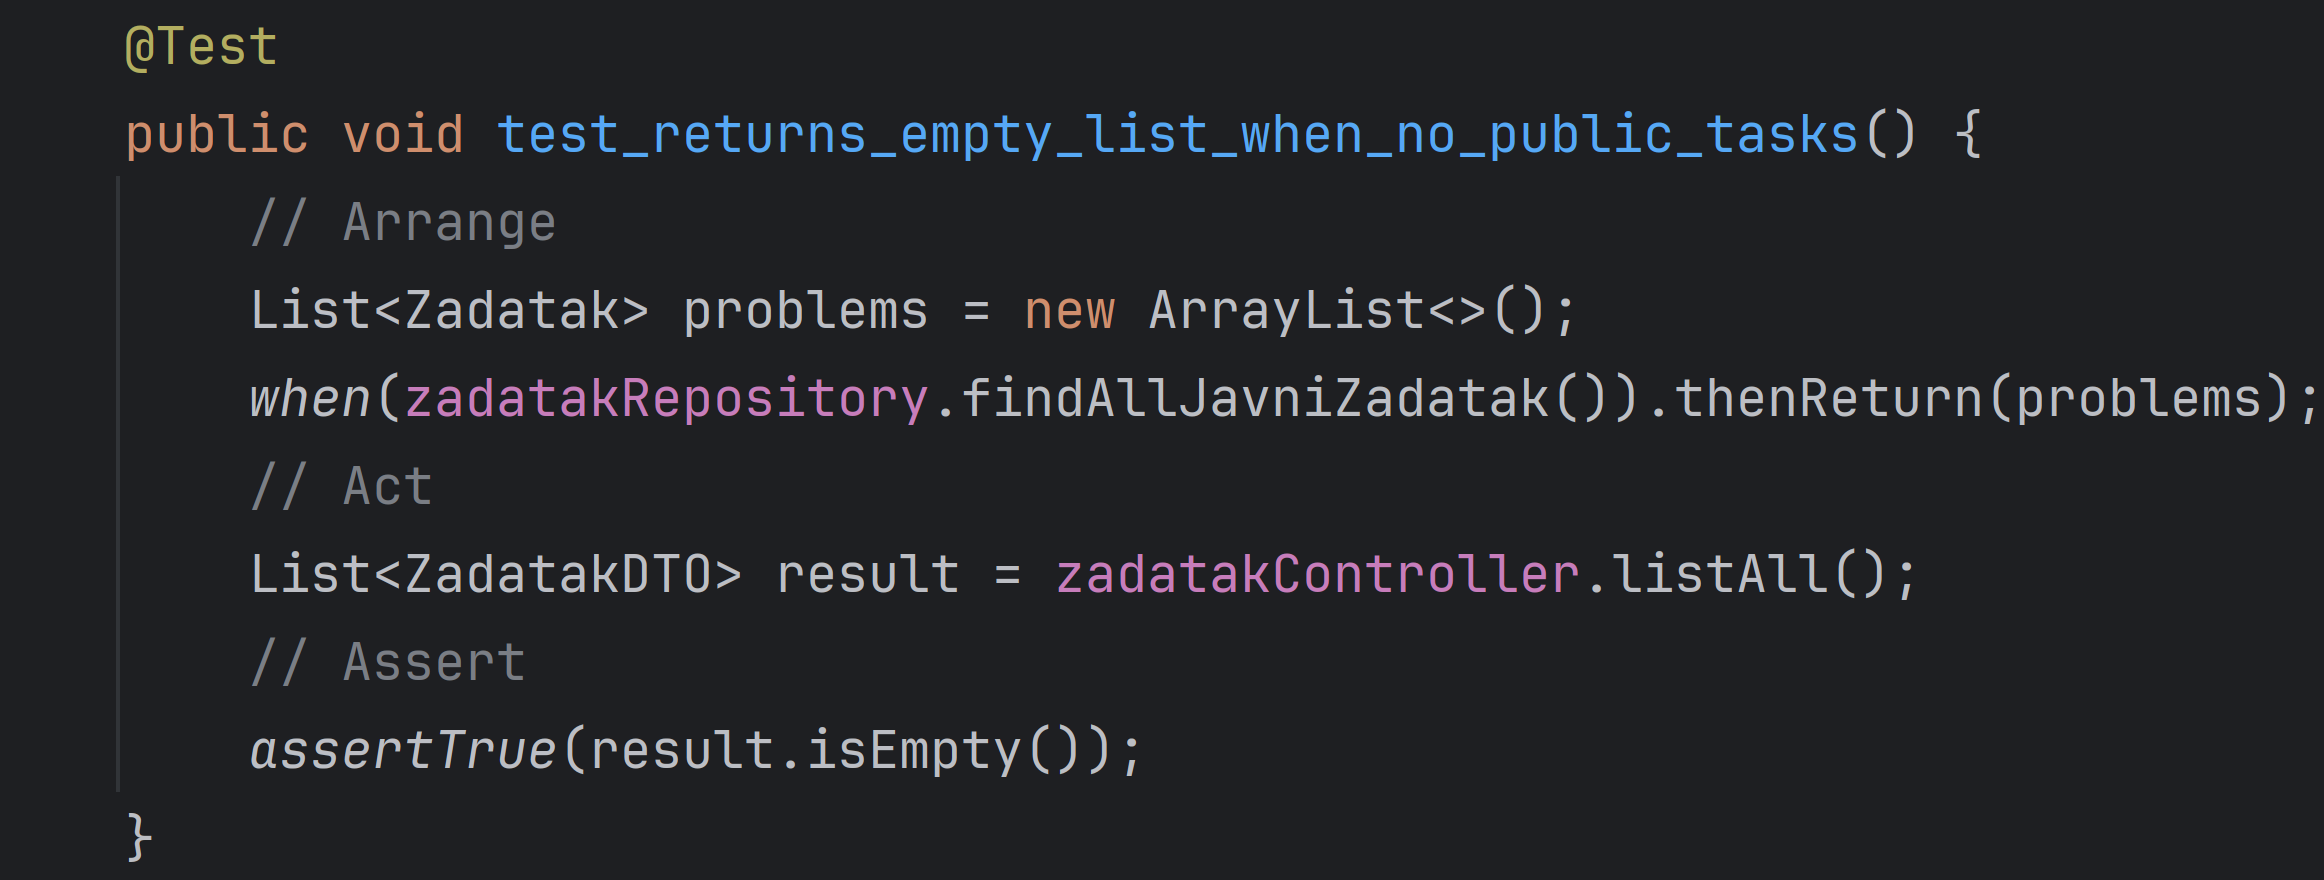
\includegraphics[scale=0.2]{slike/test6.png}
	\centering
	\caption{Testirajuća metoda - dohvat javnih zadataka}
	\label{fig:test6}
\end{figure}

Posljednjom testirajućom metodom \ref{fig:test7} ispitujemo funkcionalnost metode za ažuriranje zadatka u scenariju kada administrator želi izvršiti ažuriranje. Testiranoj metodi \textit{updateKorisnik} prosljeđujemo identifikator zadatka, podatke koje želimo ažurirati (naziv i težina) te informacije o prijavljenom korisniku (administratoru). Očekujemo da će kao izlaz metoda vratiti ažurirani objekt tipa \textit{Zadatak} te provjeravamo je su li naziv zadatka i težina zadatka ispravno ažurirani prema zadanim promjenama.


\begin{figure}[H]
	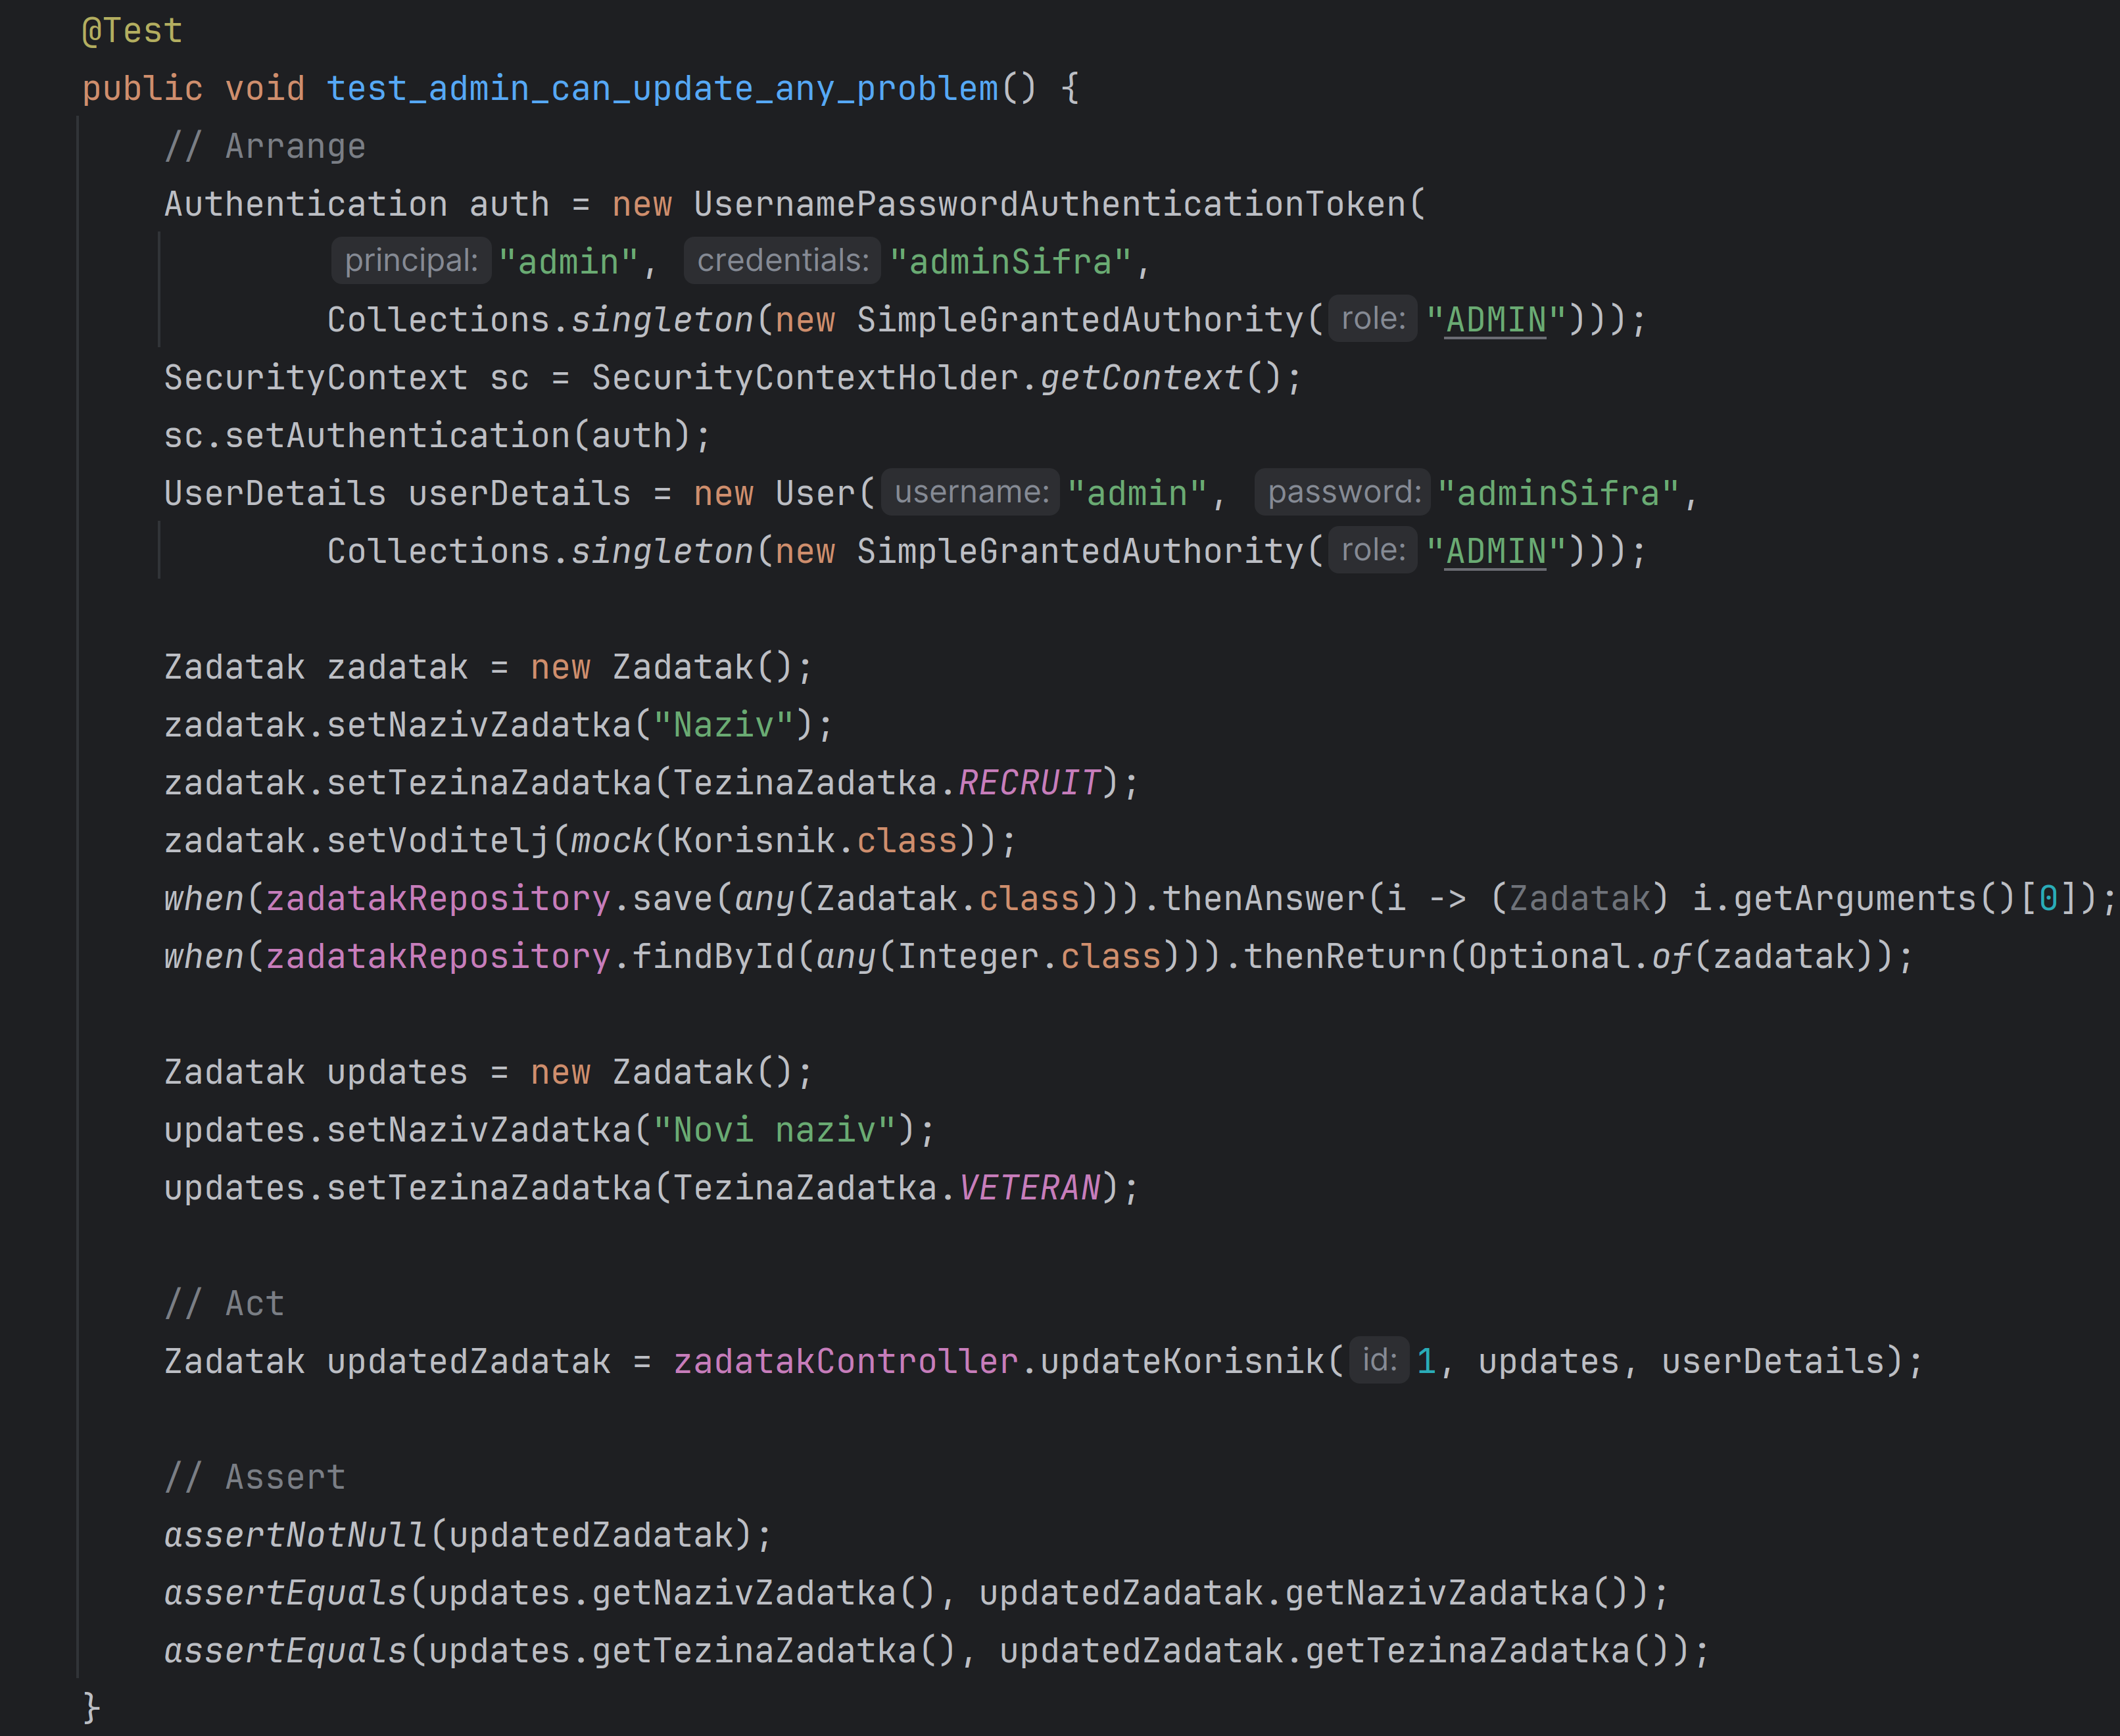
\includegraphics[scale=0.13]{slike/test7.png}
	\centering
	\caption{Testirajuća metoda - ažuriranje zadatka od strane administratora}
	\label{fig:test7}
\end{figure}

\noindent Rezultati testiranja se mogu vidjeti na slici \ref{fig:test_rezultati}.

\begin{figure}[H]
	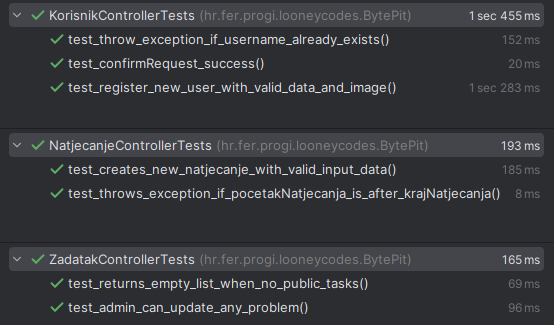
\includegraphics[scale=0.8]{slike/test_rezultati.png}
	\centering
	\caption{Rezultati testiranja}
	\label{fig:test_rezultati}
\end{figure}

\subsection{Ispitivanje sustava}

Ispitivanje sustava proveli smo pomoću \textit{Selenium Web Drivera}, implementirajući ispitne slučajeve unutar \textit{JUnit} testova. Ukupno smo napisali tri testna slučaja.

\vspace{1em}

Ispitnim slučajem \ref{fig:selenium1} ispitali smo uspješnost prijave korisnika s točnim korisničkim imenom i lozinkom te potvrdili očekivano preusmjeravanje na početnu stranicu i prisutnost gumba za odjavu.


\begin{figure}[H]
	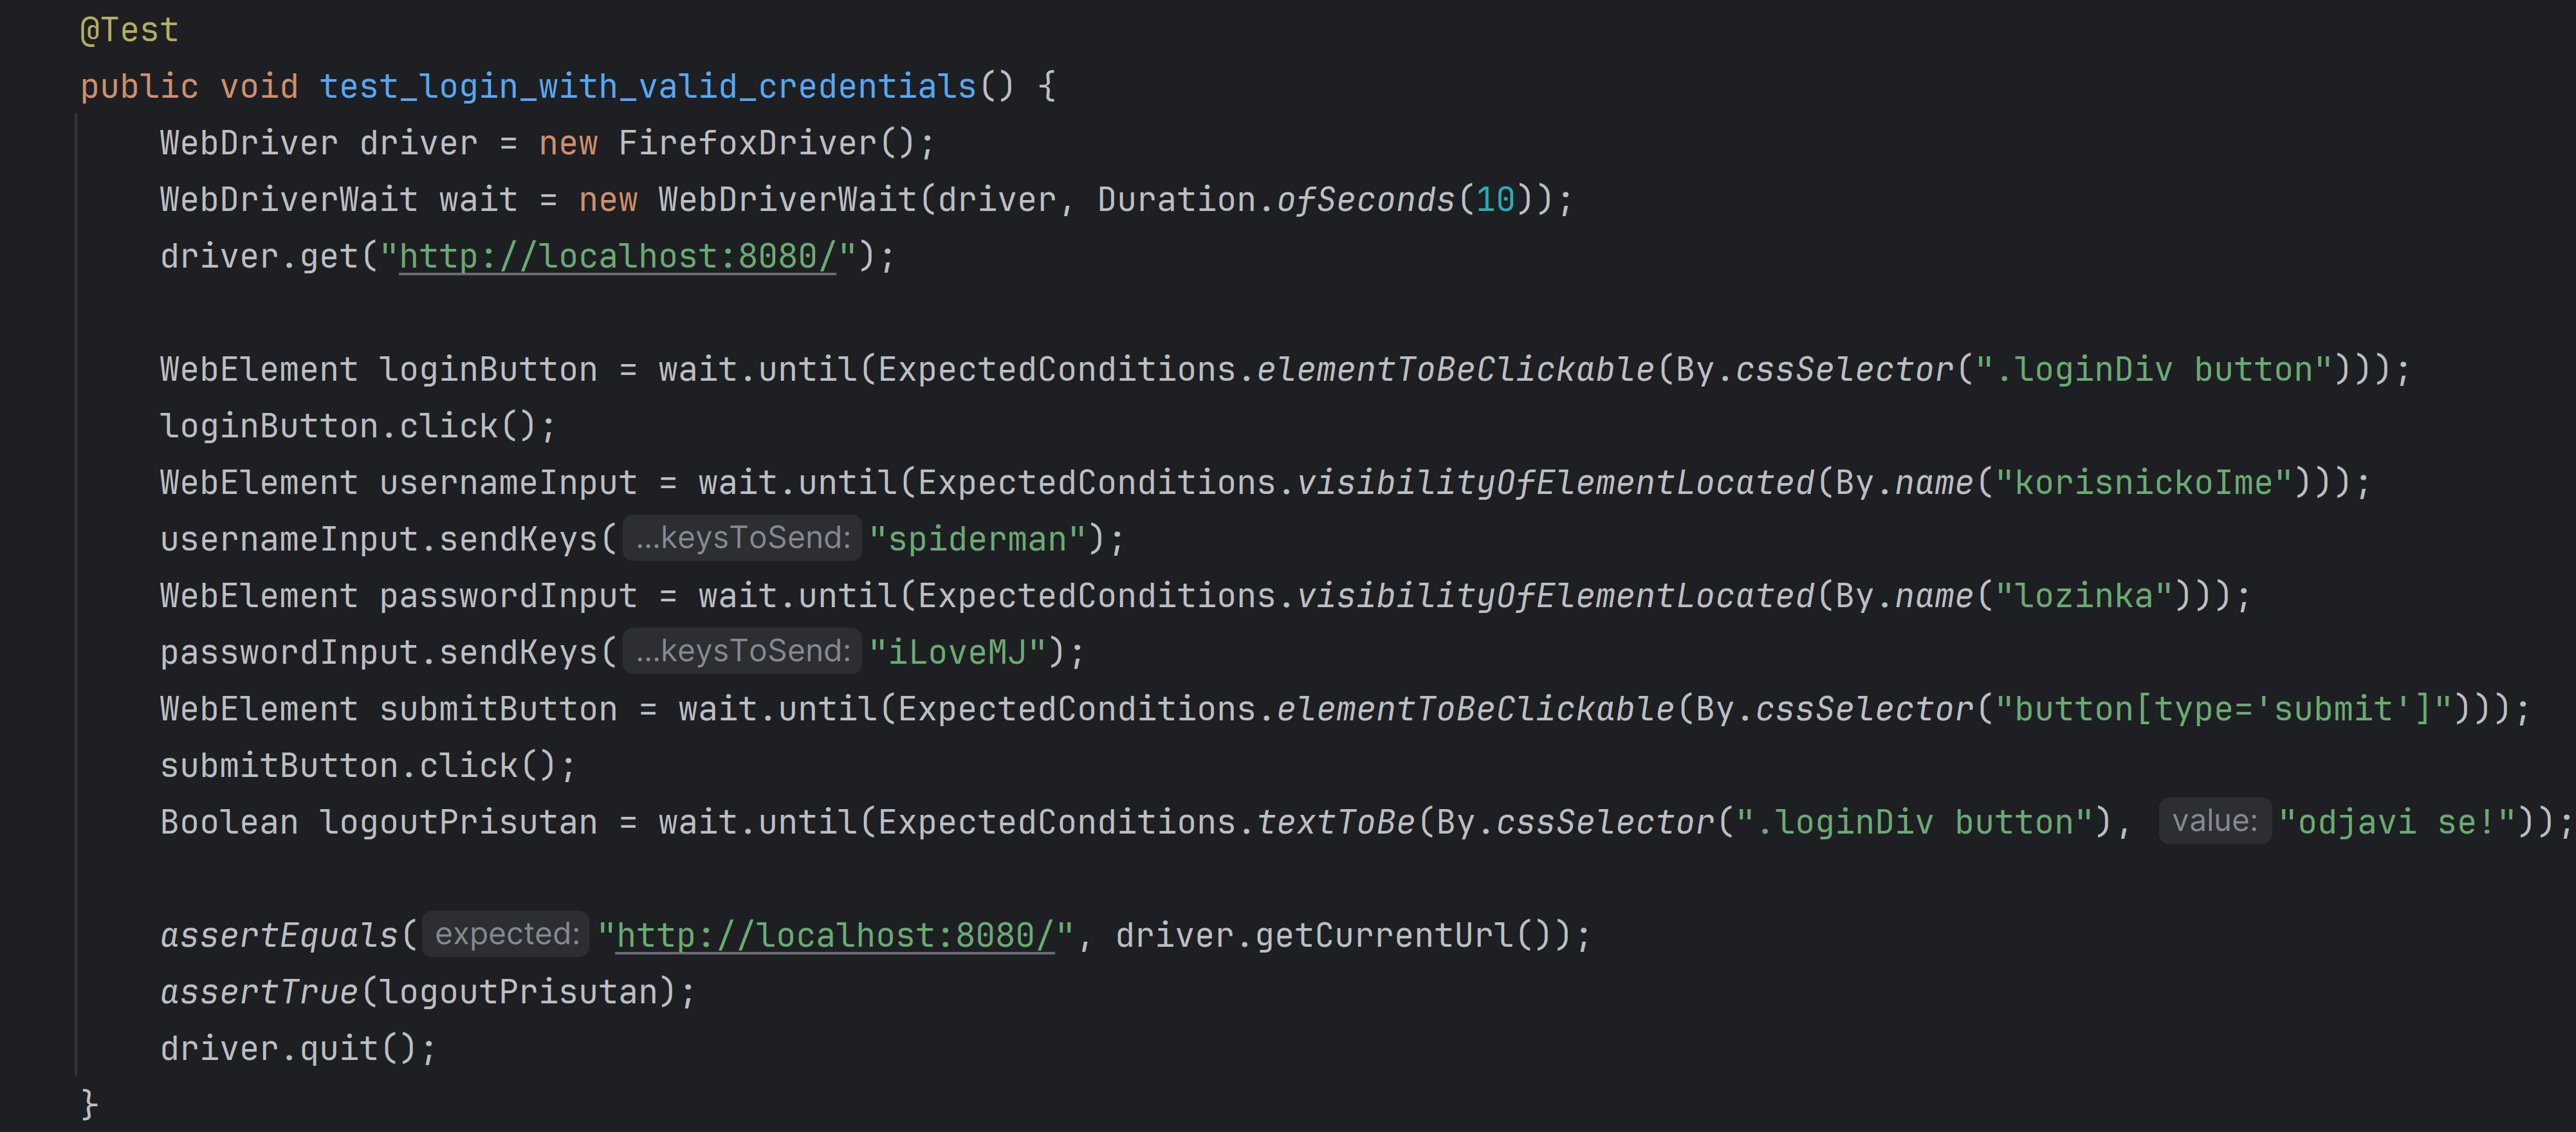
\includegraphics[scale=0.15]{slike/selenium_test1.png}
	\centering
	\caption{Selenium test - prijava korisnika s ispravnim podacima}
	\label{fig:selenium1}
\end{figure}

Testom \ref{fig:selenium2} ispitali smo ponašanje sustava prilikom pokušaja prijave s nepostojećim korisničkim imenom i lozinkom. U takvim slučajevima očekujemo zadržavanje na stranici za prijavu.

\begin{figure}[H]
	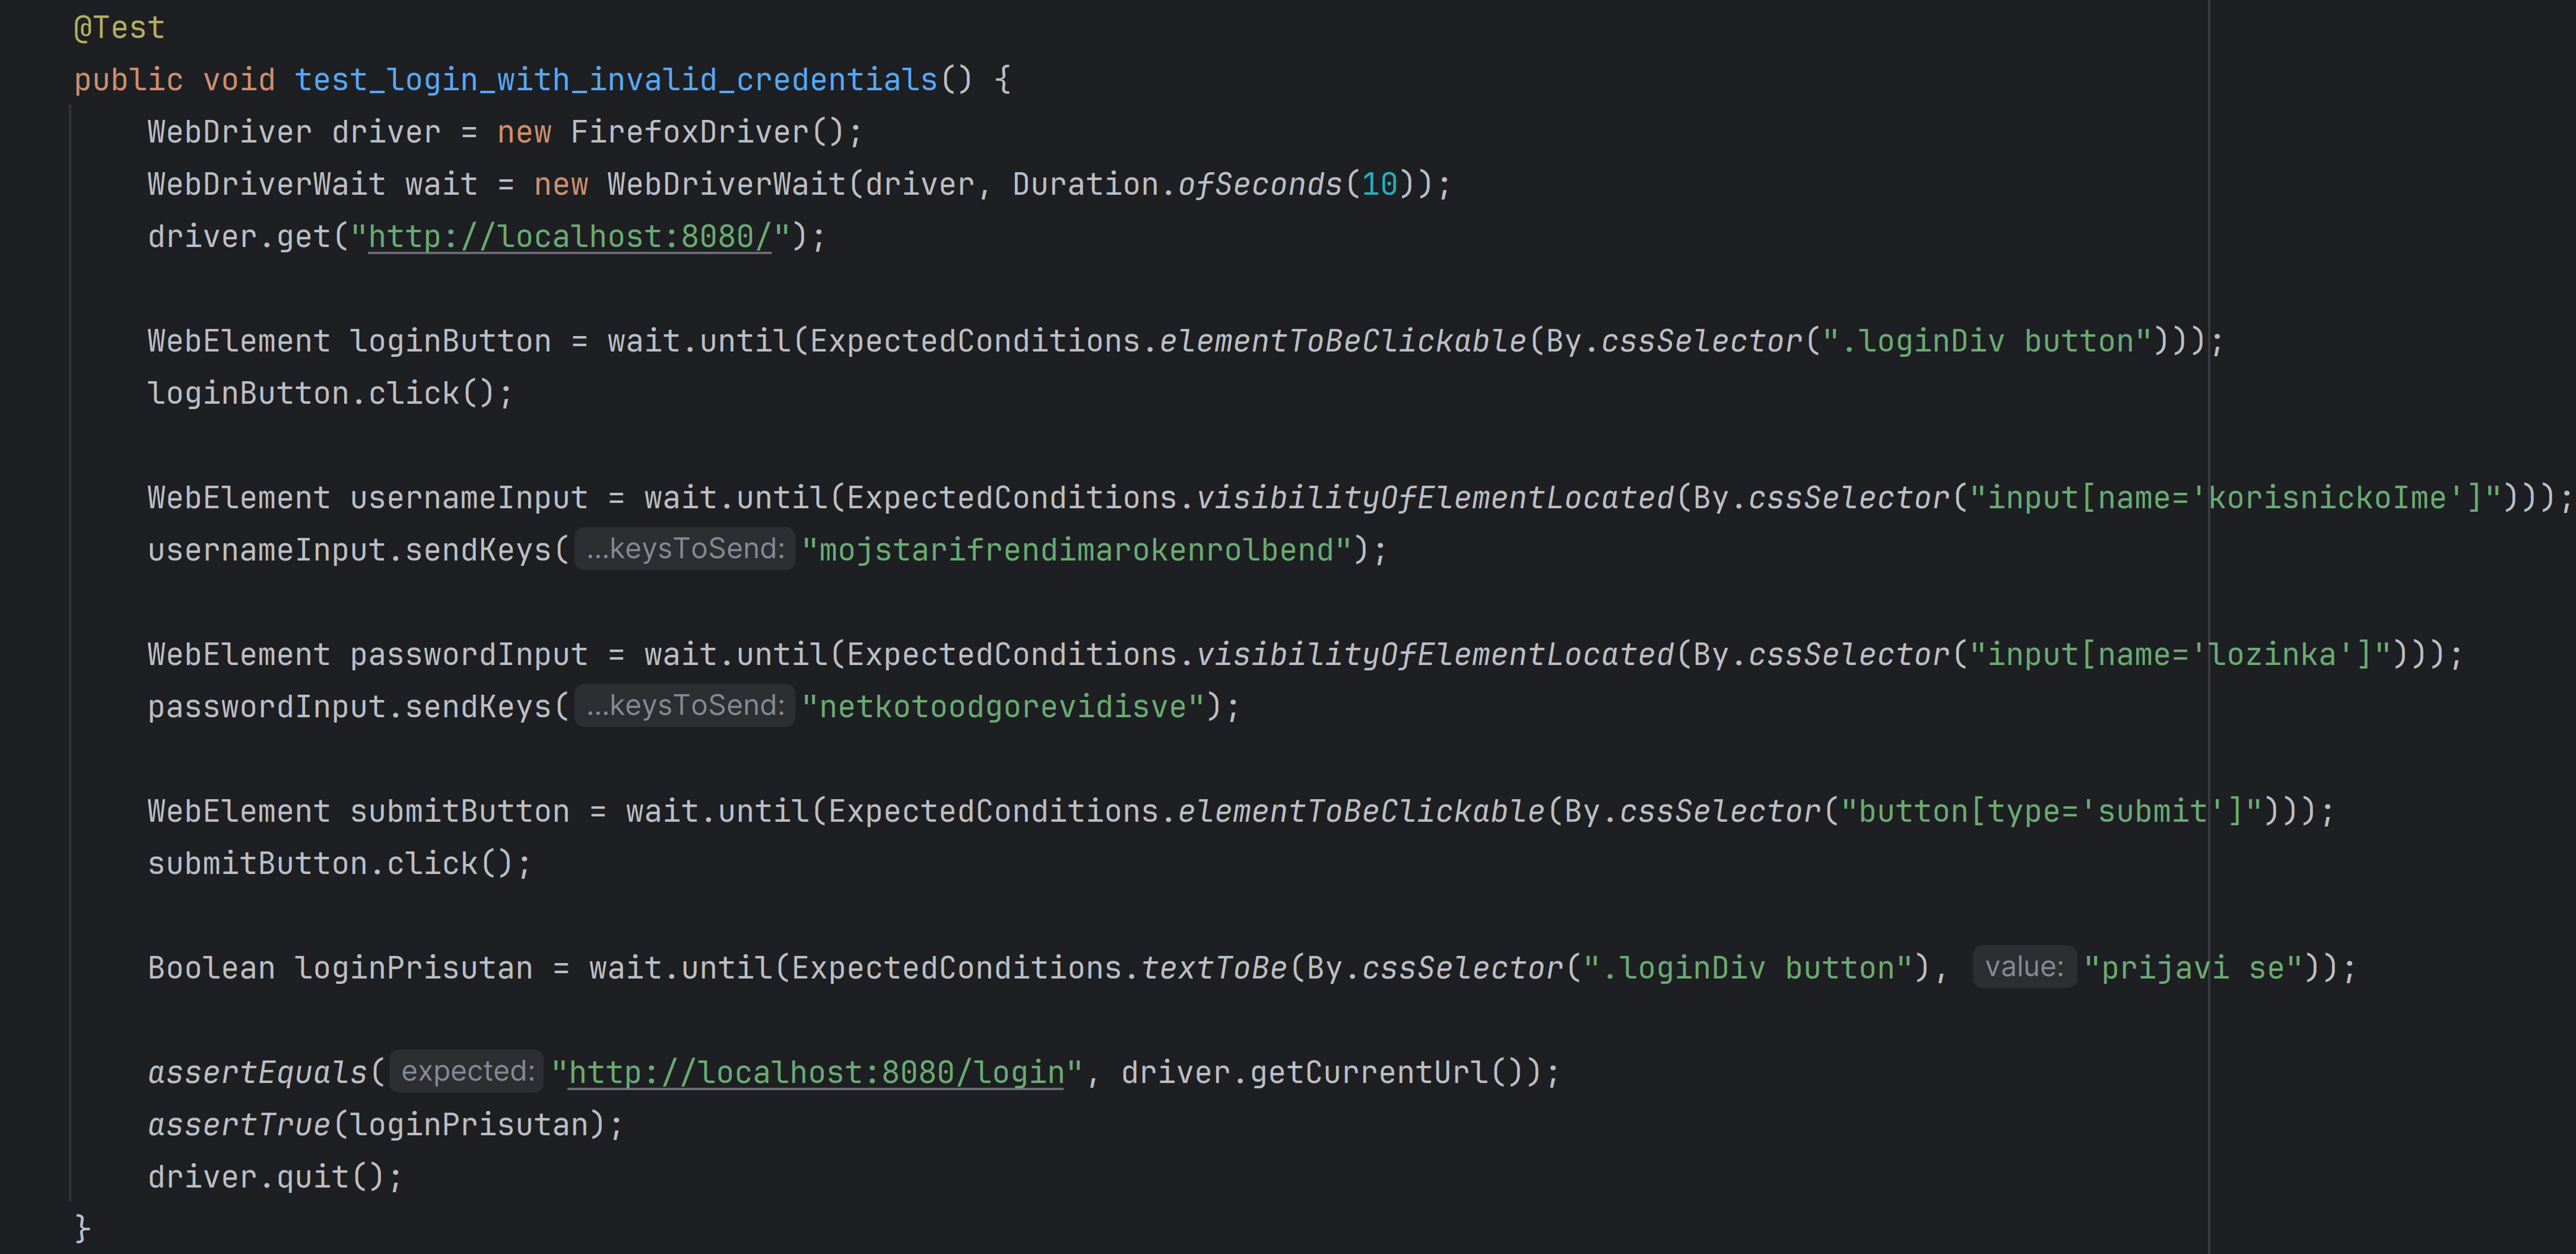
\includegraphics[scale=0.16]{slike/selenium_test2.png}
	\centering
	\caption{Selenium test - pokušaj prijave nepostojećeg korisnika}
	\label{fig:selenium2}
\end{figure}
\pagebreak
Ispitni slučaj \ref{fig:selenium3} provjerava ispravnost stvaranja novog zadatka od strane prijavljenog voditelja. Kao rezultat očekujemo pojavljivanje novostvorenog zadatka na korisničkom profilu voditelja.

\begin{figure}[H]
	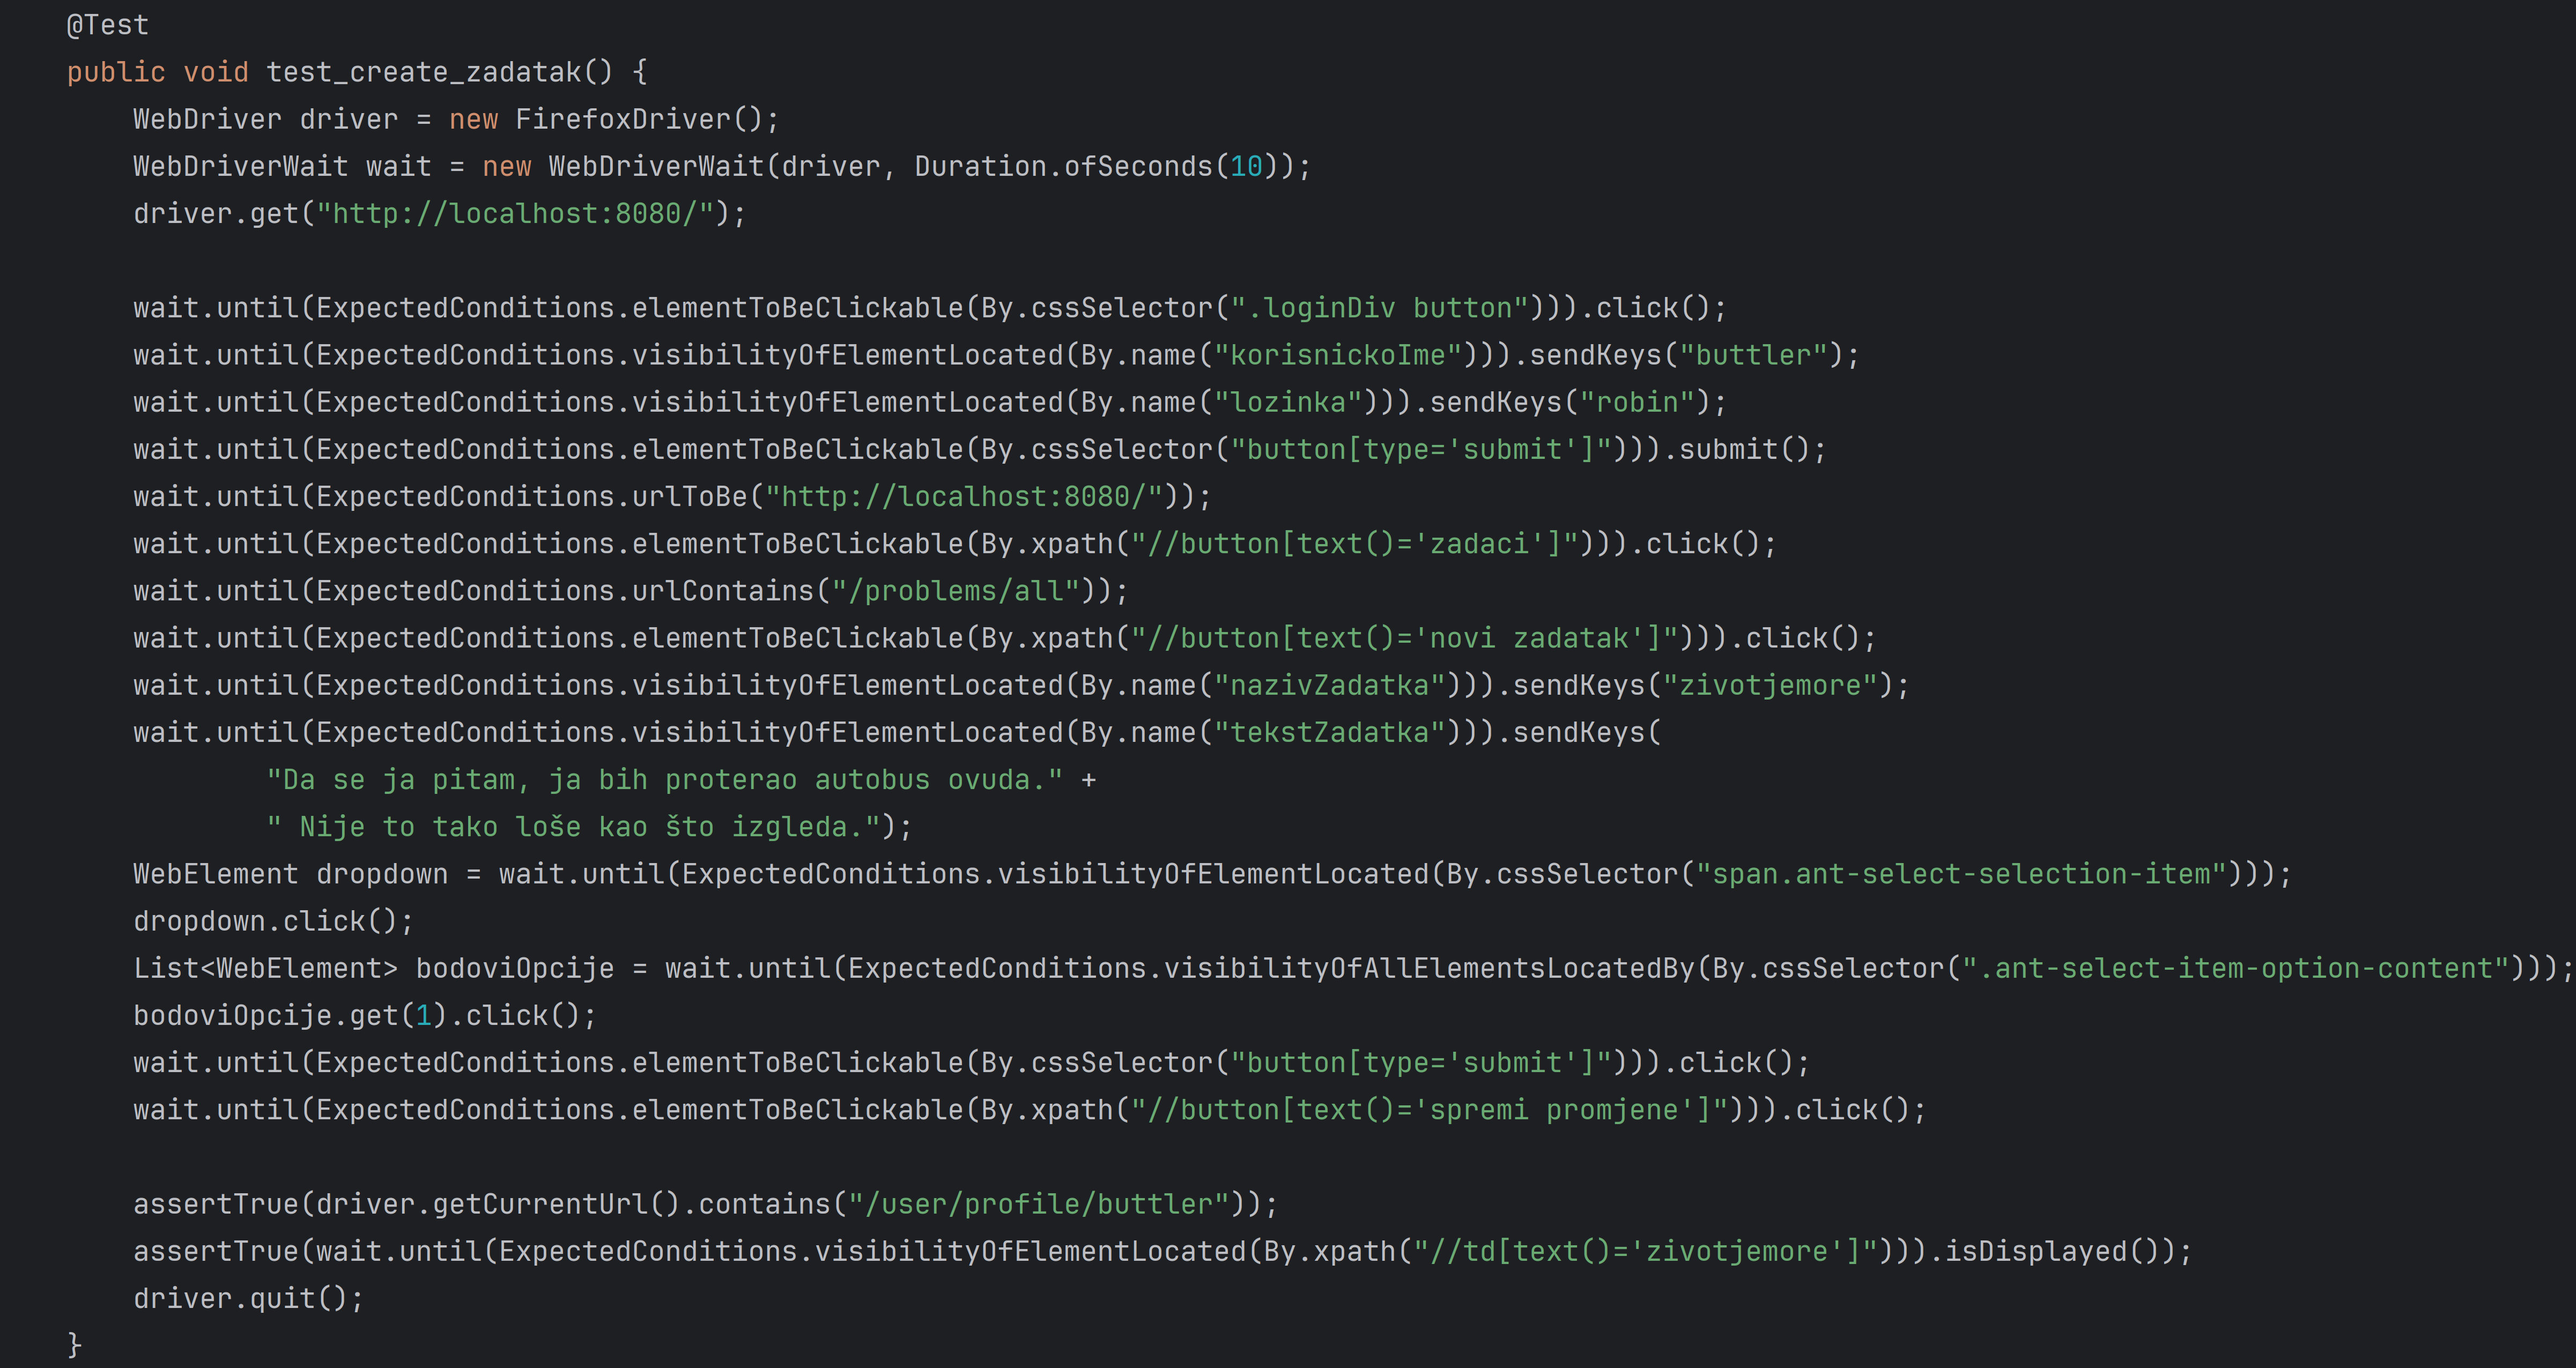
\includegraphics[scale=0.14]{slike/selenium_test3.png}
	\centering
	\caption{Selenium test - dodavanje novog zadatka}
	\label{fig:selenium3}
\end{figure}

\noindent Rezultati ispitivanja sustava se mogu vidjeti na slici \ref{fig:selenium_rezultati}.

\begin{figure}[H]
	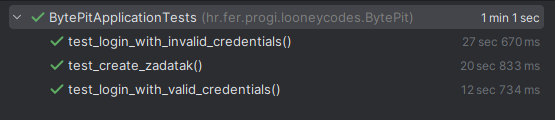
\includegraphics[scale=0.8]{slike/selenium_reultati.png}
	\centering
	\caption{Rezultati testiranja}
	\label{fig:selenium_rezultati}
\end{figure}


%\textit{Izradu ispitnih slučajeva pomoću radnog okvira Selenium moguće je provesti pomoću jednog od sljedeća dva alata:}
%\begin{itemize}
%	\item \textit{dodatak za preglednik \textbf{Selenium IDE} - snimanje korisnikovih akcija radi automatskog ponavljanja ispita	}
%	\item \textit{\textbf{Selenium WebDriver} - podrška za pisanje ispita u jezicima Java, C\#, PHP koristeći posebno programsko sučelje.}
%\end{itemize}
%\textit{Detalji o korištenju alata Selenium bit će prikazani na posebnom predavanju tijekom semestra.}

\eject



\section{Dijagram razmještaja}

UML-dijagrami razmještaja prikazuju fizičku arhitekturu i konfiguraciju razmještaja programskog sustava, a pomažu u planiranju održavanja, nadogradnji sustava, identifikaciji potencijalnih uskih grla i pojedinačnih točaka kvara. U našem primjeru, na poslužiteljskom računalu nalaze se Render web poslužitelj i poslužitelj baze podataka PostgreSQL. Poslužiteljsko računalo komunicira s klijentskim računalom putem protokola HTTPS, a na klijentskom računalu pristupamo aplikaciji putem odabranog web preglednika. Osim s klijentskim računalom, poslužiteljsko računalo komunicira i sa servisom za slanje emailova Mailjet, a koristi se i API za evaluaciju programskog rješenja kojeg predaju natjecatelji Judge0.

\begin{figure}[H]
	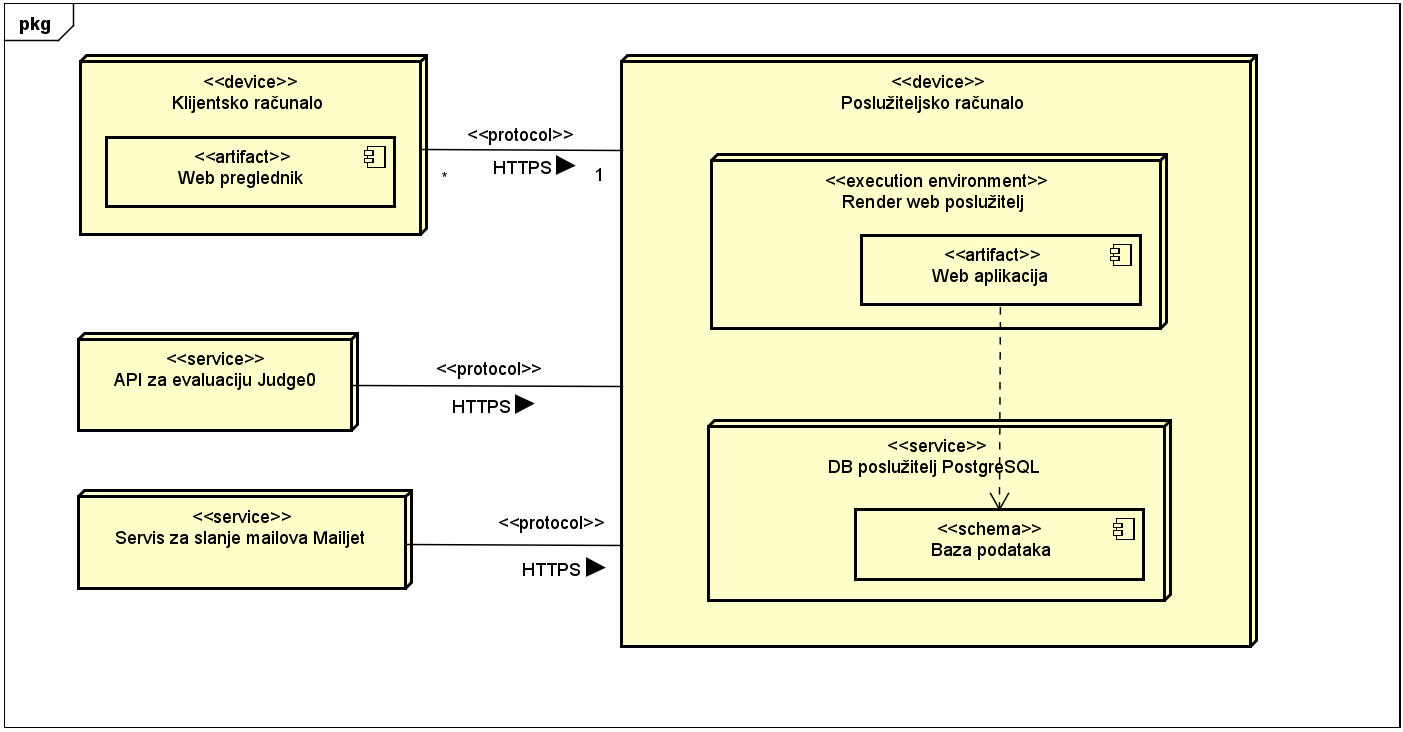
\includegraphics[scale=0.70]{dijagrami/dijagram_razmjestaja}
	\centering
	\caption{Dijagram razmještaja}
\end{figure}

\eject

\section{Upute za puštanje u pogon}

\textbf{\textit{dio 2. revizije}}\\

\textit{U ovom poglavlju potrebno je dati upute za puštanje u pogon (engl. deployment) ostvarene aplikacije. Na primjer, za web aplikacije, opisati postupak kojim se od izvornog kôda dolazi do potpuno postavljene baze podataka i poslužitelja koji odgovara na upite korisnika. Za mobilnu aplikaciju, postupak kojim se aplikacija izgradi, te postavi na neku od trgovina. Za stolnu (engl. desktop) aplikaciju, postupak kojim se aplikacija instalira na računalo. Ukoliko mobilne i stolne aplikacije komuniciraju s poslužiteljem i/ili bazom podataka, opisati i postupak njihovog postavljanja. Pri izradi uputa preporučuje se \textbf{naglasiti korake instalacije uporabom natuknica} te koristiti što je više moguće \textbf{slike ekrana} (engl. screenshots) kako bi upute bile jasne i jednostavne za slijediti.}


\textit{Dovršenu aplikaciju potrebno je pokrenuti na javno dostupnom poslužitelju. Studentima se preporuča korištenje neke od sljedećih besplatnih usluga: \href{https://aws.amazon.com/}{Amazon AWS}, \href{https://azure.microsoft.com/en-us/}{Microsoft Azure} ili \href{https://www.heroku.com/}{Heroku}. Mobilne aplikacije trebaju biti objavljene na F-Droid, Google Play ili Amazon App trgovini.}


\eject 
	\chapter{Zaključak i budući rad}
		
\noindent Zadatak naše grupe bio je razvoj web aplikacije za provjeru riješenih programskih zadataka i
sudjelovanje u natjecanjima. Razvoj aplikacije trajao je nešto više od 3 mjeseca. Proces razvoja podijeljen je u dvije faze.

		U prvoj fazi fokusirali smo se na definiranje zahtjeva, okupljanje tima, podjelu tima na podtimove i izradu temeljne dokumentacije. Obrasci uporabe, sekvencijski dijagrami, dijagram razreda te model baze podataka pružili su jasnu viziju rješenja, olakšavajući rad podtimovima zaduženima za implementaciju (\textit{backend} i \textit{frontend}). 
		
		Druga faza bila je više fokusirana na razvoj web aplikacije. Članovi tima su samostalno radili na implementaciji rješenja, suočavajući se s izazovima vezanim uz odabrane alate i programskih jezika. Unatoč manjku iskustva u pojedinim područjima, članovi su uspješno savladali izazove, i uspjeli su ostvariti sve funkcionalnosti aplikacije. Dokumentacija, poput UML dijagrama i prateće dokumentacije, pridonijela je transparentnosti sustava, olakšavajući budućim korisnicima razumijevanje i prilagodbu. Temelji za aplikaciju, definirani u prvoj fazi, uštedjeli su vrijeme i pridonijeli efikasnosti rada članova.
		
		Komunikacija članova ostvarena je putem WhatsAppa i Discorda. Pridonijela je informiranosti tima o napretku projekta, lakšu i bržu suradnju članova tima, a zajednički rad na istom projektu bio je vrijedno iskustvo za sve sudionike. Unatoč postignućima, prepoznajemo prostor za daljnje usavršavanje aplikacije. Neka od mogućih unapređenja aplikacije su dodavanje grupa za natjecanja, dodavanje tagova za kategorije zadataka, izrada mobilne aplikacije. 
		  
		Sudjelovanje u razvoju aplikacije BytePit bilo je jedinstveno i iznimno vrijedno iskustvo svim članovima, donijelo je timu osjećaj postignuća, naglašavajući važnost koordinacije i organizacije u zajedničkom projektu. Unatoč izazovima, zadovoljni smo rezultatima i radujemo se daljnjem usavršavanju ove platforme.
		\eject 
	\chapter*{Popis literature}
		\addcontentsline{toc}{chapter}{Popis literature}
	 	
% 		\textbf{\textit{Kontinuirano osvježavanje}}
%	
%		\textit{Popisati sve reference i literaturu koja je pomogla pri ostvarivanju projekta.}
		
		
		\begin{enumerate}
			
			
			\item  Programsko inženjerstvo, FER ZEMRIS, \url{http://www.fer.hr/predmet/proinz}
						
            \item  Visual Paradigm, \url{https://www.visual-paradigm.com/}

            \item  Spring Framework Documentation, \url{https://docs.spring.io/spring-framework/reference/index.html}

            \item  ReactJS Legacy Documentation, \url{https://legacy.reactjs.org/docs/getting-started.html}

			\item  ViteJS, \url{https://vitejs.dev}
		\end{enumerate}
		
		 
	
	
	\begingroup
	\renewcommand*\listfigurename{Indeks slika i dijagrama}
	%\renewcommand*\listtablename{Indeks tablica}
	%\let\clearpage\relax
	\listoffigures
	%\vspace{10mm}
	%\listoftables
	\endgroup
	\addcontentsline{toc}{chapter}{Indeks slika i dijagrama}


	
	\eject 
		
	\chapter*{Dodatak: Prikaz aktivnosti grupe}
		\addcontentsline{toc}{chapter}{Dodatak: Prikaz aktivnosti grupe}
		
		\section*{Dnevnik sastajanja}
		
%		\textbf{\textit{Kontinuirano osvježavanje}}\\
%		
%		 \textit{U ovom dijelu potrebno je redovito osvježavati dnevnik sastajanja prema predlošku.}
		
		\begin{packed_enum}
			\item  sastanak
			
			\item[] \begin{packed_item}
				\item Datum: 18. listopada 2023.
				\item Prisustvovali: Vedran Ćutić, Antonio Glavaš, Marina Hrbud, Lara Marčec, Jakov Novak, Marko Varga, Nikola Vlahović
				\item Teme sastanka:
				\begin{packed_item}
					\item  upoznavanje
					\item  analiza zadatka
					\item  postavljanje GitHub-a
				\end{packed_item}
			\end{packed_item}
			
			\item  sastanak
			\item[] \begin{packed_item}
				\item Datum: 20. listopada 2023.
				\item Prisustvovali: Vedran Ćutić, Antonio Glavaš, Marina Hrbud, Lara Marčec, Jakov Novak, Marko Varga, Nikola Vlahović
				\item Teme sastanka:
				\begin{packed_item}
					\item  uvodni sastanak s asistentom i demonstratoricom 
					\item  razrješavanje upita o osnovnim funkcionalnostima aplikacije
					\item  dogovor oko alata i tehnologija
				\end{packed_item}
			\end{packed_item}
			
			\item  sastanak
			\item[] \begin{packed_item}
				\item Datum: 31. listopada 2023.
				\item Prisustvovali: Vedran Ćutić, Antonio Glavaš, Marina Hrbud, Lara Marčec, Jakov Novak, Marko Varga, Nikola Vlahović
				\item Teme sastanka:
				\begin{packed_item}
					\item  pregled odrađenih zadataka
					\item  dogovor o vizualnom izgledu aplikacije
					\item  raspodjela daljnjih poslova i dogovor internih rokova za iste
				\end{packed_item}
			\end{packed_item}
			
			\item  sastanak
			\item[] \begin{packed_item}
				\item Datum: 7. studenog 2023.
				\item Prisustvovali: Vedran Ćutić, Antonio Glavaš, Marina Hrbud, Lara Marčec, Jakov Novak, Marko Varga, Nikola Vlahović
				\item Teme sastanka:
				\begin{packed_item}
					\item  zajednička diskusija o dosad odrađenim zadacima
					\item  konkretna raspodjela daljnjih poslova i uloga
				\end{packed_item}
			\end{packed_item}


   			\item  sastanak
			\item[] \begin{packed_item}
				\item Datum: 15. studenog 2023.
				\item Prisustvovali: Vedran Ćutić, Antonio Glavaš, Marina Hrbud, Lara Marčec, Jakov Novak, Marko Varga, Nikola Vlahović
				\item Teme sastanka:
				\begin{packed_item}
					\item  pregled svih odrađenih zadataka
					\item  diskusija o predaji projekta 17.11.
     					\item  deployment aplikacije
				\end{packed_item}
			\end{packed_item}
			
			%
			
		\end{packed_enum}
		
		\eject
		\section*{Tablica aktivnosti}
		
			\textbf{\textit{Kontinuirano osvježavanje}}\\
			
			 \textit{Napomena: Doprinose u aktivnostima treba navesti u satima po članovima grupe po aktivnosti.}

			\begin{longtblr}[
					label=none,
				]{
					vlines,hlines,
					width = \textwidth,
					colspec={X[7, l]X[1, c]X[1, c]X[1, c]X[1, c]X[1, c]X[1, c]X[1, c]}, 
					vline{1} = {1}{text=\clap{}},
					hline{1} = {1}{text=\clap{}},
					rowhead = 1,
				} 
			

				\SetCell[c=1]{c}{} & \SetCell[c=1]{c}{\rotatebox{90}{\textbf{Vedran Ćutić }}} & \SetCell[c=1]{c}{\rotatebox{90}{\textbf{Antonio Glavaš }}} &	\SetCell[c=1]{c}{\rotatebox{90}{\textbf{Marina Hrbud }}} & \SetCell[c=1]{c}{\rotatebox{90}{\textbf{Lara Marčec }}} &	\SetCell[c=1]{c}{\rotatebox{90}{\textbf{Jakov Novak }}} & \SetCell[c=1]{c}{\rotatebox{90}{\textbf{Marko Varga }}} &	\SetCell[c=1]{c}{\rotatebox{90}{\textbf{Nikola Vlahović }}} \\  

				Upravljanje projektom 		  & 2 &  &  &  &  & \\
				Opis projektnog zadatka 	&  &  & 2 &  &  & 2 & \\ 
				
				Funkcionalni zahtjevi       &  &  &  & 1 &  &  & 2\\
				Opis pojedinih obrazaca 	&  &  &  & 2 &  &  & 1\\ 
				Dijagram obrazaca 			&  &  &  &  & 2 & 1 &  \\ 
				Sekvencijski dijagrami 		&  &  &  & 4 &  &  &  \\ 
				Opis ostalih zahtjeva 		&  &  &  & 1 &  &  &  \\ 

				Arhitektura i dizajn sustava	 &  & 3 &  &  &  &  &  \\ 
				Baza podataka				&  &  & 4 &  &  & 2 &   \\ 
				Dijagram razreda 			&  & 2 &  &  &  &  &   \\ 
				Dijagram stanja				&  &  &  &  &  &  &  \\ 
				Dijagram aktivnosti 		&  &  &  &  &  &  &  \\ 
				Dijagram komponenti			&  &  &  &  &  &  &  \\ 
				Korištene tehnologije i alati 		  &  &  &  &  &  &  \\
				Ispitivanje programskog rješenja 	  &  &  &  &  &  &  \\
				Dijagram razmještaja			&  &  &  &  &  &  &  \\ 
				Upute za puštanje u pogon 		&  &  &  &  &  &  &  \\  
				Dnevnik sastajanja 			&  &  & 1 & 1 &  &  &  \\ 
				Zaključak i budući rad 		&  &  &  &  &  &  &  \\  
				Popis literature 			&  &  &  &  &  &  &  \\  
				&  &  &  &  &  &  &  \\ \hline 
				\textit{Dodatne stavke kako ste podijelili izradu aplikacije} 			&  &  &  &  &  &  &  \\ 
				\text{izrada početne stranice} 			&  &  & 10 & 10 &  &  &  \\  
				\text{izrada baze podataka} 		 	&  &  & 4 &  &  & \\
				\text{spajanje s bazom podataka} 		&  &  &  &  & 5 &  &  \\ 
		        \text{back end - servisi i controlleri}	&  &  &  &  & 15 &  & 13\\
		        \text{deployment}          				&  &  &  &  &  5 &  &\\ 
			\end{longtblr}
					
					
		\eject
%		\section*{Dijagrami pregleda promjena}
%		
%		\textbf{\textit{dio 2. revizije}}\\
%		
%		\textit{Prenijeti dijagram pregleda promjena nad datotekama projekta. Potrebno je na kraju projekta generirane grafove s gitlaba prenijeti u ovo poglavlje dokumentacije. Dijagrami za vlastiti projekt se mogu preuzeti s gitlab.com stranice, u izborniku Repository, pritiskom na stavku Contributors.}
%		
	



\end{document} %naredbe i tekst nakon ove naredbe ne ulaze u izgrađen dokument 


